%% Copyright 2007-2018 Elsevier Ltd
%% 
%% This file is part of the 'Elsarticle Bundle'.

%% ---------------------------------------------
%% 
%% It may be distributed under the conditions of the LaTeX Project Public
%% License, either version 1.2 of this license or (at your option) any
%% later version.  The latest version of this license is in
%%    http://www.latex-project.org/lppl.txt
%% and version 1.2 or later is part of all distributions of LaTeX
%% version 1999/12/01 or later.
%% 
%% The list of all files belonging to the 'Elsarticle Bundle' is
%% given in the file `manifest.txt'.
%% 
%% Template article for Elsevier's document class `elsarticle'
%% with harvard style bibliographic references

%\documentclass[preprint,12pt,authoryear]{elsarticle}

%\documentclass[twocolumn,12pt,authoryear]{elsarticle}
%% Use the option review to obtain double line spacing
%\documentclass[authoryear,preprint,review,12pt]{elsarticle}

%% Use the options 1p,twocolumn; 3p; 3p,twocolumn; 5p; or 5p,twocolumn
%% for a journal layout:
%%\documentclass[final,1p,times,authoryear]{elsarticle}
%%\documentclass[final,1p,times,twocolumn,authoryear]{elsarticle}
%%\documentclass[final,3p,times,authoryear]{elsarticle}
\documentclass[final,3p,twocolumn]{elsarticle}
%%\documentclass[final,5p,times,authoryear]{elsarticle}
%%\documentclass[final,5p,times,twocolumn,authoryear]{elsarticle}

%% For including figures, graphicx.sty has been loaded in
%% elsarticle.cls. If you prefer to use the old commands use
%%\usepackage{epsfig}
%% The amssymb package provides various useful mathematical symbols
\usepackage{amssymb}
%% The amsthm package provides extended theorem environments
 \usepackage{amsthm}
%\usepackage{graphicx}% Include figure files
%\usepackage{pdflscape}
 \usepackage[figuresright]{rotating}
 \usepackage{hyperref}
 \usepackage{subfig}
 \usepackage{lineno}
 \usepackage{natbib}
%\usepackage{array}
%\usepackage{dcolumn,multirow}
% Align table columns on decimal point
%% The lineno packages adds line numbers. Start line numbering with \begin{linenumbers} and end with \end{linenumbers}
%% Or switch it on

%\linenumbers
%\journal{Nuclear Instruments and Methods A}
\begin{document}
\begin{frontmatter}
%% Title, authors and addresses
%% use the tnoteref command within \title for footnotes;
%% use the tnotetext command for theassociated footnote;
%% use the fnref command within \author or \addoratorytnote;
%% use the corref command within \author for corresponding author footnotes;
%% use the cortext command for theassociated footnote;
%% use the ead command for the email address,
%% and the form \ead[url] for the home page:
%% \title{Title\tnoteref{label1}}
%% \tnotetext[label1]{}
%% \author{Name\corref{cor1}\fnref{label2}}
%% \ead{email address}
%% \ead[url]{home page}
%% \fntext[label2]{}
%% \cortext[cor1]{}
%% \address{Address\fnref{label3}}
%% \fntext[label3]{}

  \title{The CLAS12 Spectrometer at Jefferson Laboratory}
%% use optional labels to link authors explicitly to addresses:
%% \author[label1,label2]{}
%% \address[label1]{}
%% \address[label2]{}
\author{V.D. Burkert, L. Elouadrhiri, D. Anderson, S. Aune, H. Avakian, N. Baltzell, M. Battaglieri,  V. Baturin,
  S. Boiarinov, P. Bonneau, K. Bruhwel, D.S. Carman, A. Celentano, M. Contalbrigo, S. Christo, M. Defurne, G. Dodge,
  R. De Vita, K. Giovanetti, F.X. Girod, L. Guo, R. Gothe, Y. Gotra, K. Hafidi, D. Heddle, P. Hemler, K. Hicks, D. Insley, K. Joo,
  D. Kashy, A. Kim, W. Kim, V. Kubarovsky, S. Kuhn, M. Mcmullen, I. Mandjavidze, N. Markov, C. Mealer, M. Mestayer,
  Z.E. Meziani, R. Miller, M. Mirazita, S. Niccolai, O. Pastor, E. Pasyuk, O. Pogorelko, B. Raue, P. Rossi, F. Sabatie,
  Y. Sharabian, D. Sokhan, S. Stepanyan, M. Ungaro, A. Vlassov, D. Watts, L. Weinstein, C. Wiggins, A. Yegneswaran, 
  G. Young, M. Zarecky, V. Ziegler, {\bf incomplete list} ......... more coming ............. }
%\address{12000 Jefferson Avenue, Newport News, Virginia, 23606}
%\author{ K. Hafidi,  .......} 
%\address{ Argonne National Laboratory, Argonne, Illinois, 60439, USA}
%\author{D. Heddle, ........}
%\address{Christopher Newport University, Newport News, Virginia 23605, USA} 
%\author{K. Joo, A. Kim, N. Markov, ........} 
%\address{University of Connecticut, Storrs, Connecticut 06269, USA} 
%\author{A. Biselli,..}
%\address{Fairfield University, Fairfield, Connecticut 06824, USA}
%\author{L. Guo, B. Raue, ...}
%\address{Florida International University, Miami, Florida, 33199, USA} 
%\author{S. Aune, M. Defurne, I. Mandjavidze, F. Sabatie, ....... }
%\address{IRFU, CEA, Universit{\'e} Paris-Saclay, F-91191 Gif-sur-Yvette, France}
%\author{M. Battaglieri, A. Celentano, R. De Vita, .....}
%\address{INFN, Sezione di Genova, 16146 Genova, Italy}
%\author{P. Chatagnon, S. Niccolai, ......}
%\address{Institut de Physique Nucl{\'e}aire, IN2P3-CNRS, Universit{\'e} Paris-Sud,  Universit{\'e} Paris-Saclay,
 % F-91406 Orsay, France}
%\author{O. Pogorelko, A. Vlassov, ....} 
%\address{Institute of Theoretical and Experimental Physics, Moscow, Russia}
%\author{G. Dodge, S. Kuhn, L. Weinstein,  Victoria xxx, ........}
%\address{Old Dominion University, Norfolk, Virginia, 23529, USA} 
%\author{R. Gothe, ...................}
%\address{University of South Carolina, Columbia, South Carolina 29208}
%\author{ K. Hicks, ....} 
%\address{ Ohio University, Athens, Ohio, 45701}
%\author{P. Cole, T. Forrest, K. Hicks, .........}
%\address{Idaho State University, Pocatello, Idaho, 83209, USA}
%\author{M. Contalbrigo, .......}
%\address{INFN, Sezione di Ferrara, 44100 Ferrara, Italy}  
%\author{M. Mirazita, .......}
%\address{INFN, Laboratori Nazionali di Frascati, 00044 Frascati, Italy}
%\author{K. Giovanetti, ......}
%\address{James Madison University, Harrisonburg, Virginia 22807, USA}
%\author{W. Kim, .....}
%\address{Kyungpook National University, Daegu 41566, Republic of Korea}
%\address{ .......................................... }
%\vspace{-0.5cm}

\begin{abstract}
The CEBAF Large Acceptance Spectrometer for operation at 12~GeV beam energy (CLAS12) at Jefferson 
Laboratory is used to study electro-induced nuclear and hadronic reactions, and provides efficient detection of
charged and neutral particles over a large fraction of the full solid angle. CLAS12 has been part of the
energy-doubling project of Jefferson Lab's Continuous Wave Electron Beam Accelerator Facility, funded by the
United States Department of Energy. A collaboration of over 40 institutions contributed to the design and
construction of detector hardware, developed the software packages for the simulation of complex event patterns,
and commissioned the detector systems. CLAS12 is based on a dual-magnet system with a superconducting Torus
magnet that provides a largely azimuthal field distribution that covers the forward angle range, and a solenoid magnet
and detector covering the polar angles from $40^\circ$ to $125^\circ$, with full azimuthal coverage. Trajectory
reconstruction in the forward direction using drift chambers and in the central direction using a vertex tracker
results in momentum resolutions of $< 1\%$ and $< 3\%$, respectively.  Cherenkov counters, time-of-flight
scintillators, and electromagnetic calorimeters provide good particle identification. Fast triggering and high
data-acquisition rates allow operation at a luminosity of $10^{35}$~cm$^{-2}$s$^{-1}$. These capabilities are being
used in a broad program to study the structure and interactions of nucleons, nuclei, and mesons, using polarized and
unpolarized electron beams and targets for beam energies up to 11~GeV. This paper gives a general description of
the design, construction, and performance of CLAS12.  
\end{abstract}

\end{frontmatter}

\nolinenumbers
\section{Introduction}
%\label{Intro}

Electron scattering has been proven an effective way of probing the size and internal structure of subatomic
particles as protons, neutrons, and nuclei. Exploiting energetic electron beams led to rapid progress in our
understanding of the internal composition of particles. The extended size of the proton was first mapped out in
the mid-1950's~\cite{Mcallister:1956ng}, and the internal quark substructure was discovered in the late 1960's
\cite{Breidenbach:1969kd}. Using spin-polarized electrons and spin-polarized targets, the internal quark helicity
momentum distribution was mapped out in the 1980's and the following decades, and is still an important research
topic today~\cite{Kuhn:2008sy}. These experiments only required inclusive measurements, where only the beam
particle, electrons or muons, that scattered off the target were detected and kinematically analyzed.  

\begin{figure*}[ht]
\centerline{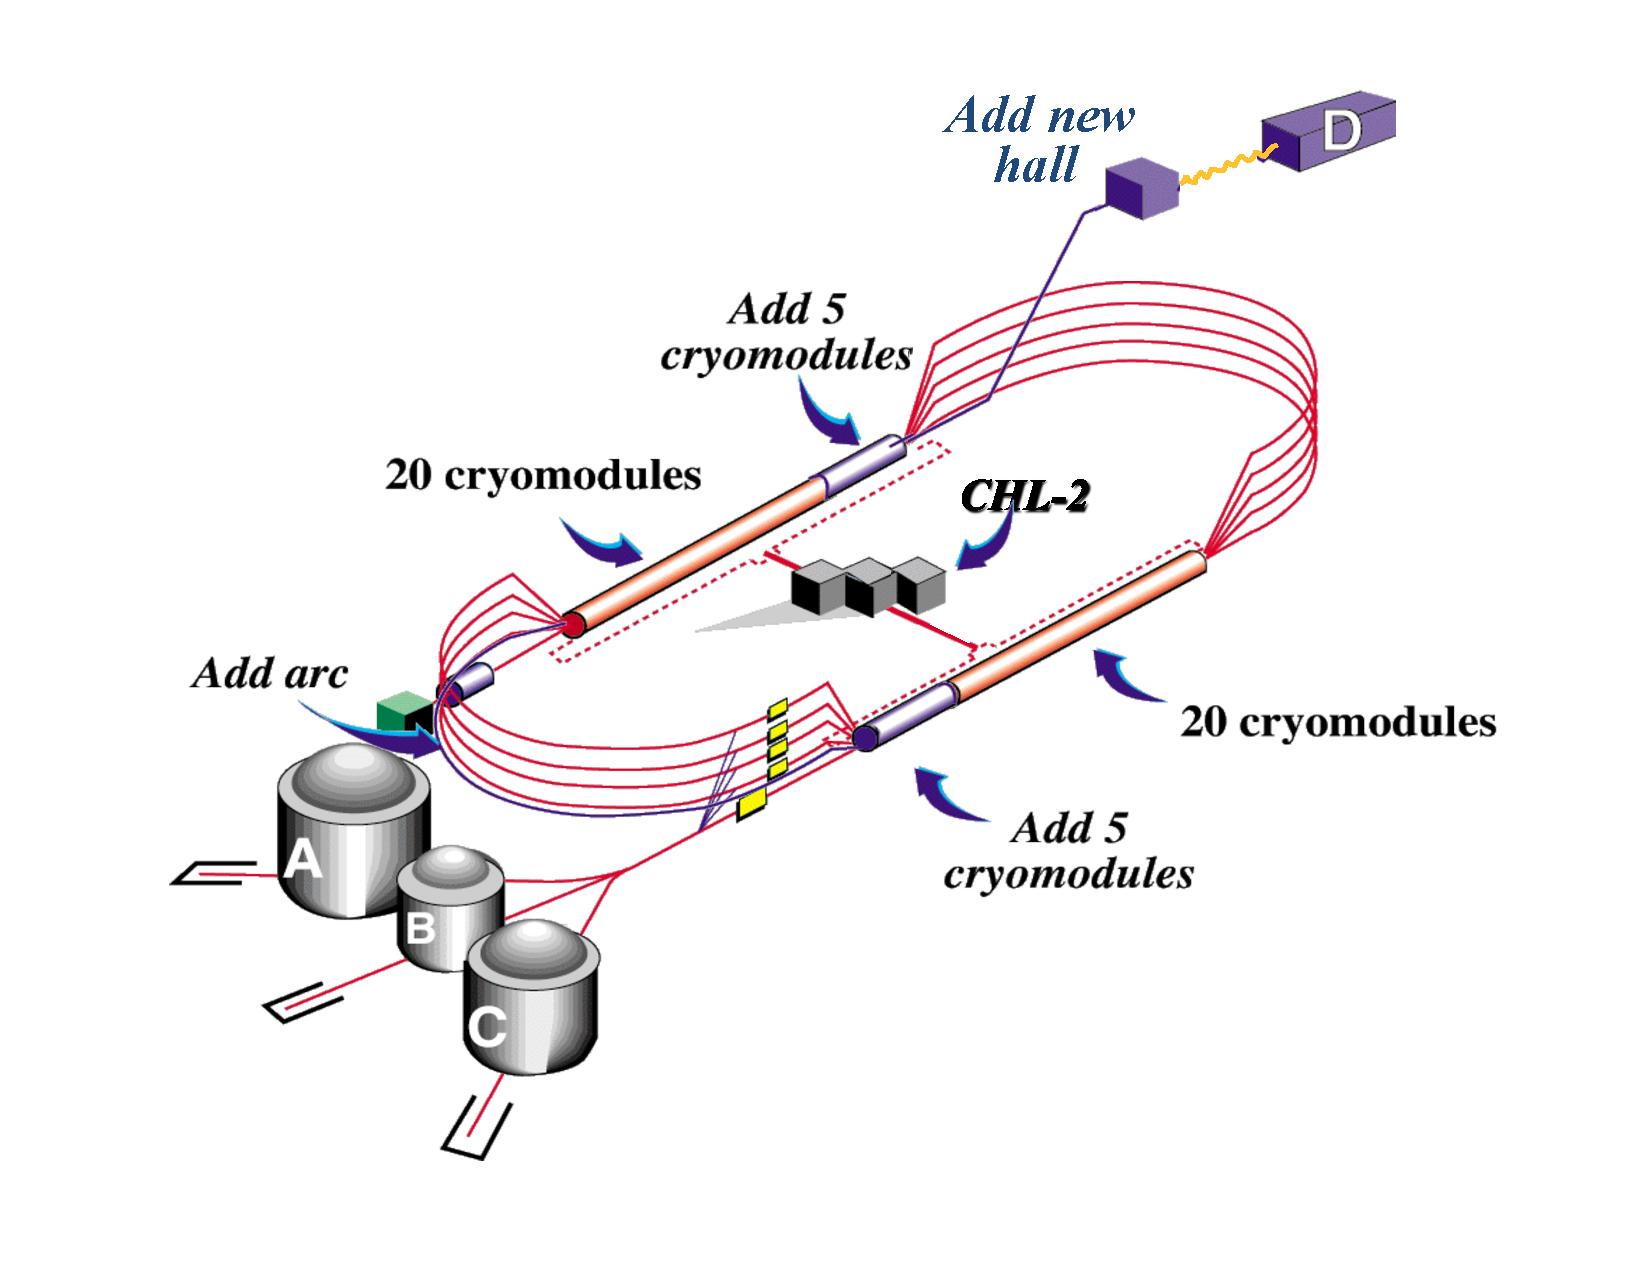
\includegraphics[width=1.8\columnwidth]{cebaf.pdf}}
\caption{ (Color Online) The CEBAF continuous electron beam accelerator after the doubling of the beam energy to 12~GeV and 
adding Hall~D as a new experimental end station for photon physics experiments.The accelerator is 1,400~m in
circumference.}
\label{cebaf12}
\end{figure*} 

In the decades following these discoveries, it was realized that a more detailed understanding of the internal
structure of nucleons requires the reconstruction of fully exclusive or semi-inclusive processes, and hence the
detection and kinematical reconstruction of additional mesons and baryons in the final state was required.  Other
constraints came from the desire of baryon spectroscopy to measure complete angular distributions, which made it
necessary to employ large acceptance devices to serve that purpose. The Continuous Electron Beam Accelerator
Facility (CEBAF)~\cite{Leemann:2001dg}, the CLAS detector~\cite{Mecking:2003zu}, and other experimental
equipment at Jefferson Laboratory (JLab) were designed and constructed in the 1990's with these goals in mind
and were operated successfully for over 15 years. 

The further development of Quantum Chromodynamics (QCD) as the theory of the interaction of colored quarks and
gluons, combined with the discovery of the Generalized Parton Distributions (GPDs) provided a novel way that allowed
describing the nucleon structure in 3 dimensions (3D), 2 in coordinate space and 1 in momentum space. The discovery
opened up a new avenue of hadronic research that has become one of the flagship programs in nuclear and hadronic
physics. The GPDs must be probed in exclusive processes, with deeply virtual Compton scattering being the most
suitable one, and in a large kinematic space. This is a rather rare process and measurements require high-intensity
electron (or muon) beams and large acceptance detectors to provide sufficient rate to map out the process in the full
kinematic phase space using polarized beams, polarized targets, and sufficiently high beam energy. The complementary
process of semi-inclusive deep inelastic scattering (SIDIS) is also of topical interest,  which also probes the nucleon's
internal structure in 3D momentum space. The science program of CLAS12 is very broad~\cite{Burkert:2018nvj} and
encompasses the study of the structure of the proton and neutron both in their ground state, as well as their many
excited states, and in the deeply inelastic kinematics. Other experiments are designed to probe the short range
structure of nuclei through measurements of the transparency of nuclei to mesons and baryons, and how it changes
with the momentum transfer.   

\begin{figure*}[t]
\centering
\centerline{\includegraphics[width=1.8\columnwidth]{CLAS12-side-3.png}}
\caption{(Color Online) The CLAS12 detector in the Hall~B beamline. The electron beam enters from the right and impinges on
the production target located in the center of the solenoid magnet shown at the right (upstream) end of CLAS12,
where other detector components are also visible. Scattered electrons and forward-going particles are detected
in the Forward Detector (FD) consisting of a high-threshold Cherenkov counter (HTCC) with full coverage in polar
angle $5^\circ \le \theta \le 35^\circ$ and $\Delta \phi = 2\pi$ coverage in azimuth. The HTCC is followed by the
Torus magnet, the drift chamber (DC) tracking system, another set of Cherenkov counters (LTCC, RICH),
time-of-flight scintillation counters (FTOF), and electromagnetic calorimeters (ECAL). The DCs are supported from
the Torus magnet. The detectors downstream of the Torus magnet are mounted on a separate Forward Carriage that
is independently movable to allow access to the detectors for maintenance. The Central Detector (CD) consists of the
Silicon Vertex Tracker (SVT), which is surrounded by a Barrel Micromesh Tracker (BMT), the Central Time-of-Flight
(CTOF) counter, and the Central Neutron Detector (CND). The entire CLAS12 detector extends for 20~m along the
beamline.} 
\label{clas12}
\end{figure*}

\begin{figure*}[bhtp!]
\centerline{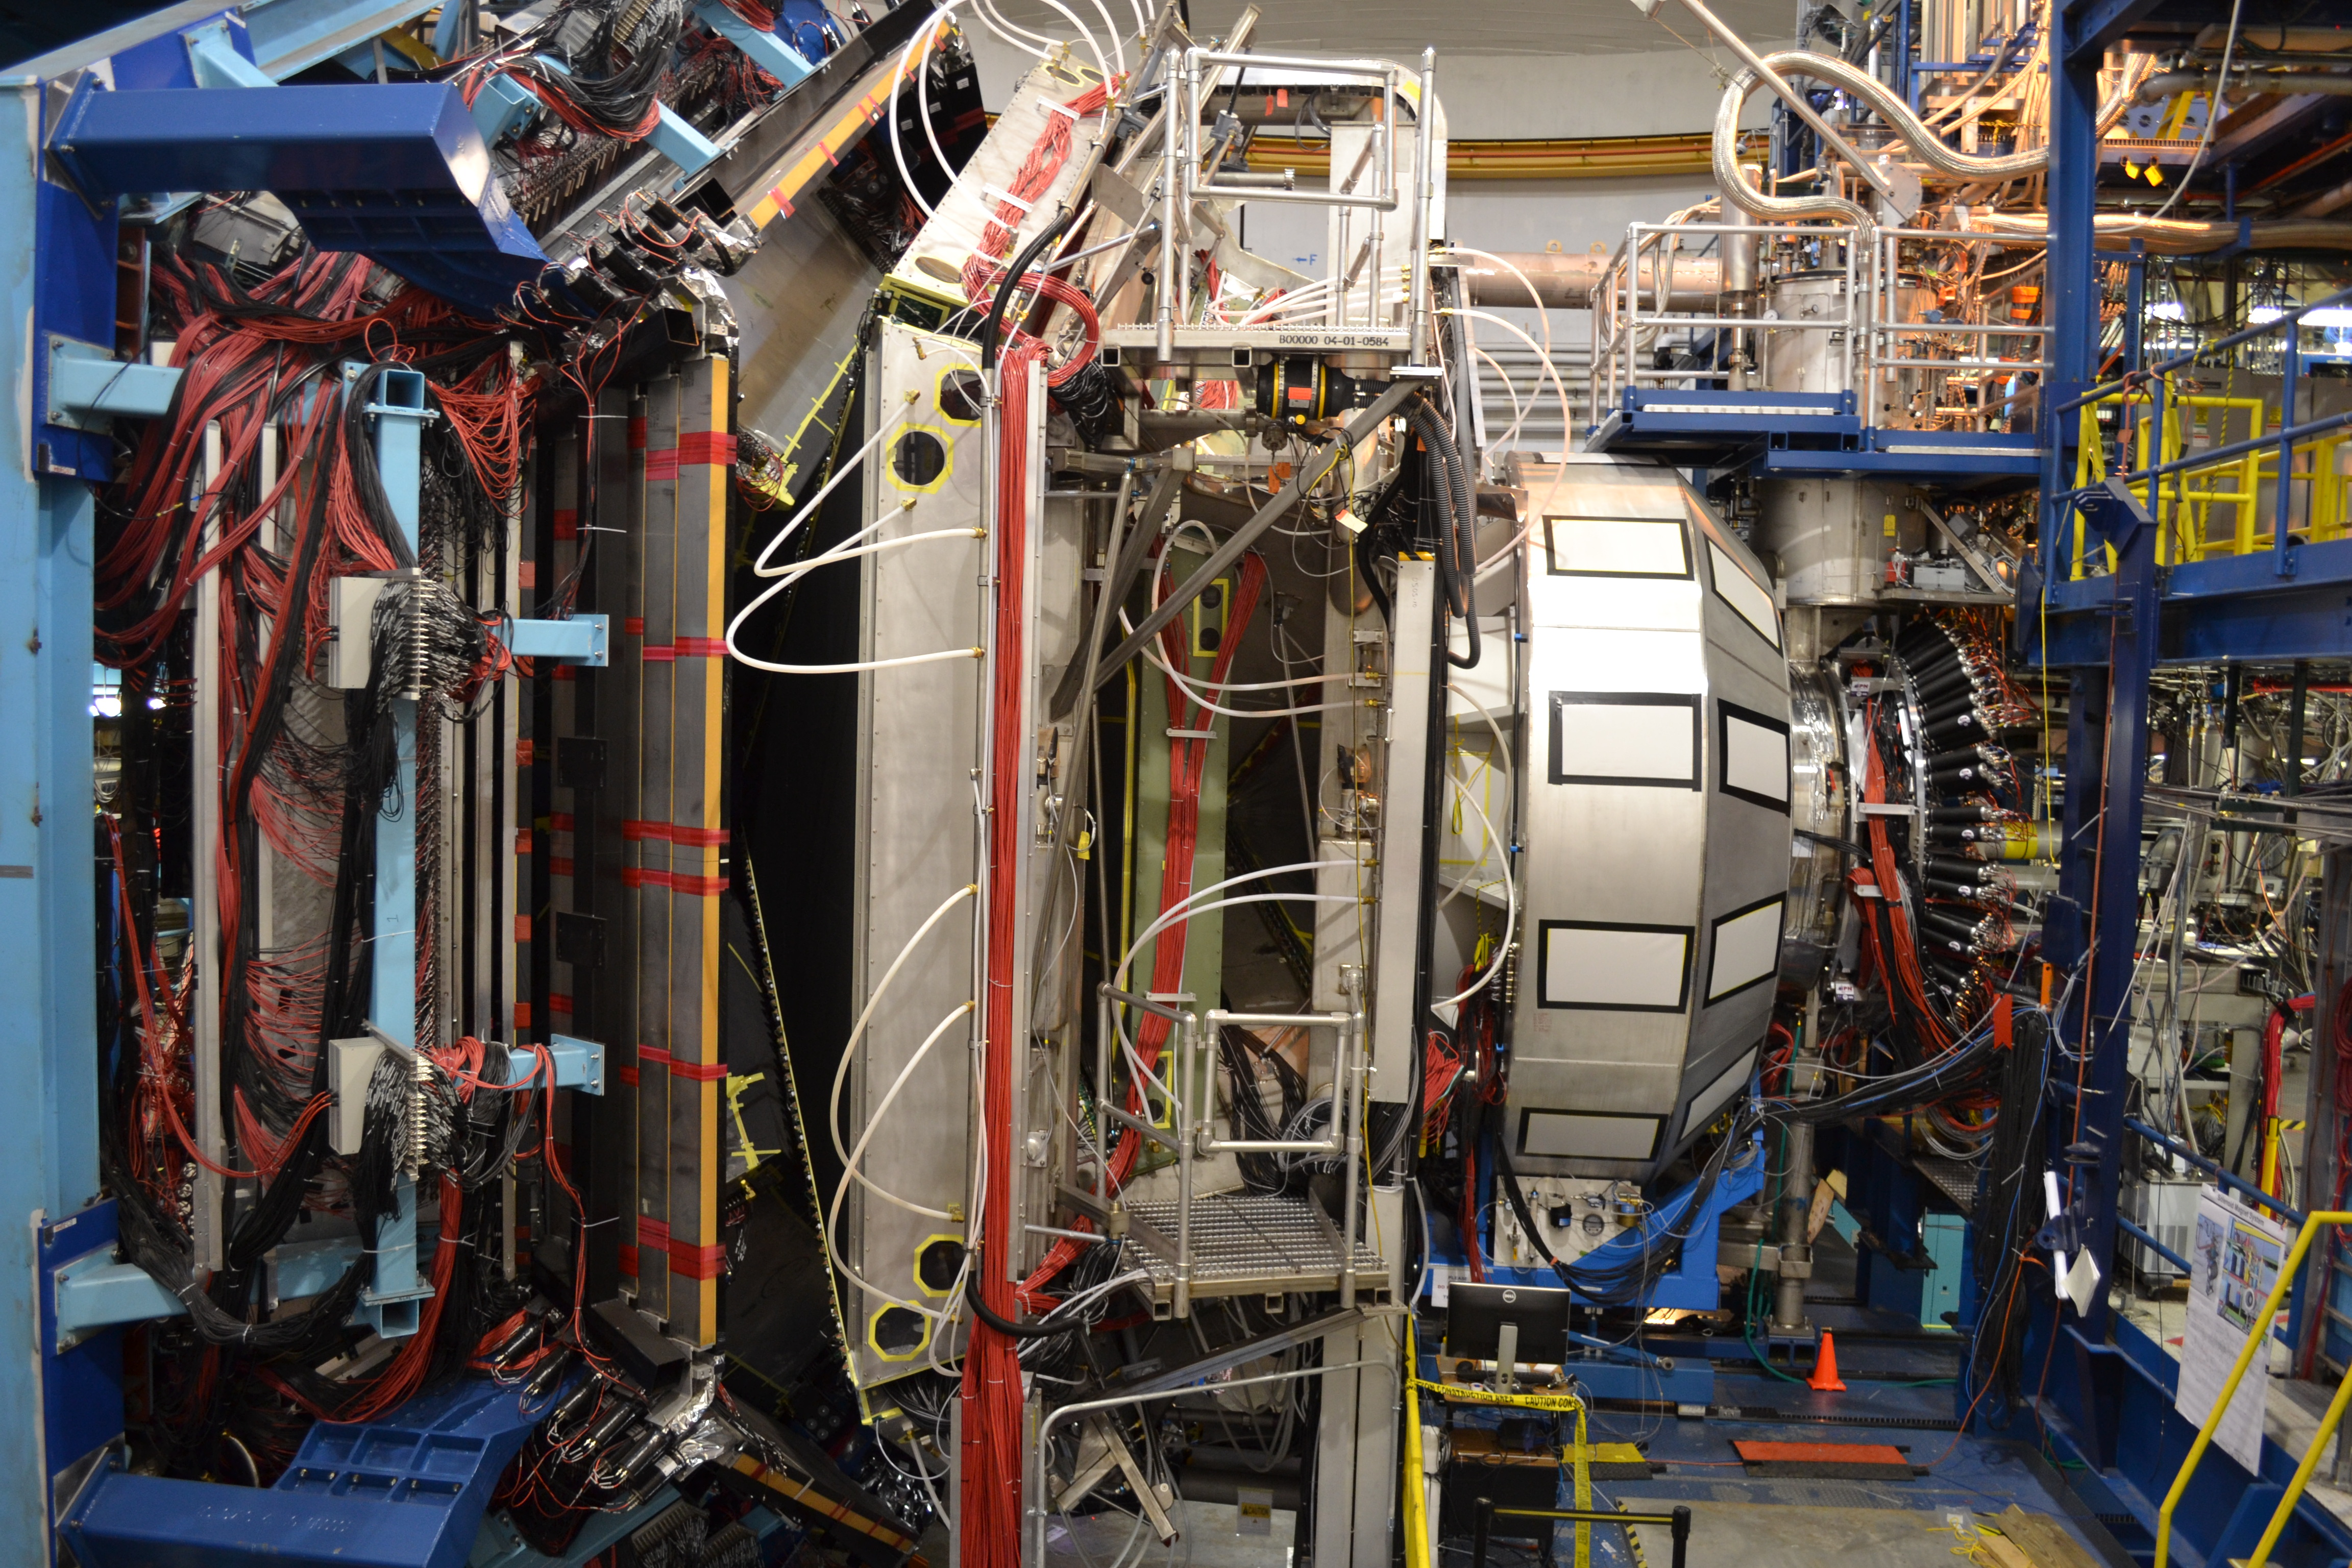
\includegraphics[width=1.4\columnwidth]{CLAS12_photo-1.jpg}}
\caption{(Color Online) The CLAS12 detector in the Hall~B beamline. The beam enters from the right near the upstream end of the
Solenoid magnet and the cryogenic service tower, followed by the HTCC and the Torus magnet with the drift chambers.
The LTCC, FTOF, and the calorimeters, PCAL and EC, are seen at the downstream end to the left.}
\label{clas12-photo}
\end{figure*}
\section{The Jefferson Laboratory Facility at 12~GeV}
\label{jlab}

The CLAS12 detector was designed to study electro-induced nuclear and hadronic reactions by providing efficient
detection of charged and neutral particles over a large fraction of the full solid angle. A collaboration of over 40
institutions has participated in the design, fabrication, assembly, and final commissioning of CLAS12 in Hall~B at the
Thomas Jefferson  National Accelerator Facility. The CLAS12 detector is based on a combination of a six-coil Torus
magnet and a high-field Solenoid magnet. The combined magnetic field provides a large coverage in both azimuthal and
polar angles. Trajectory reconstruction using drift chambers at forward angles results in a momentum resolution of
${\sigma_p / p} \approx 0.005$. At large polar angles, where particle momenta are typically below 1~GeV, the vertex
resolution is $\approx 200-300~\mu\rm{m}$ ({\bf put correct values in} ) with momentum resolutions of
$\sigma_p / p \approx 0.03$  ({\bf put correct values here}).  Cherenkov counters, time-of-flight systems, and
calorimeters provide good particle identification for electrons, charged pions, kaons, and protons. Fast triggering and
high data acquisition rates allow operation in luminosities of $10^{35}~\rm{cm}^{-2}\rm{s}^{-1}$ for extended periods of
time. These capabilities are being used in a broad scientific program to study the structure and interactions of baryons,
meson, and nuclei using polarized and unpolarized targets. 

\begin{figure*}[htbp!]
\centerline{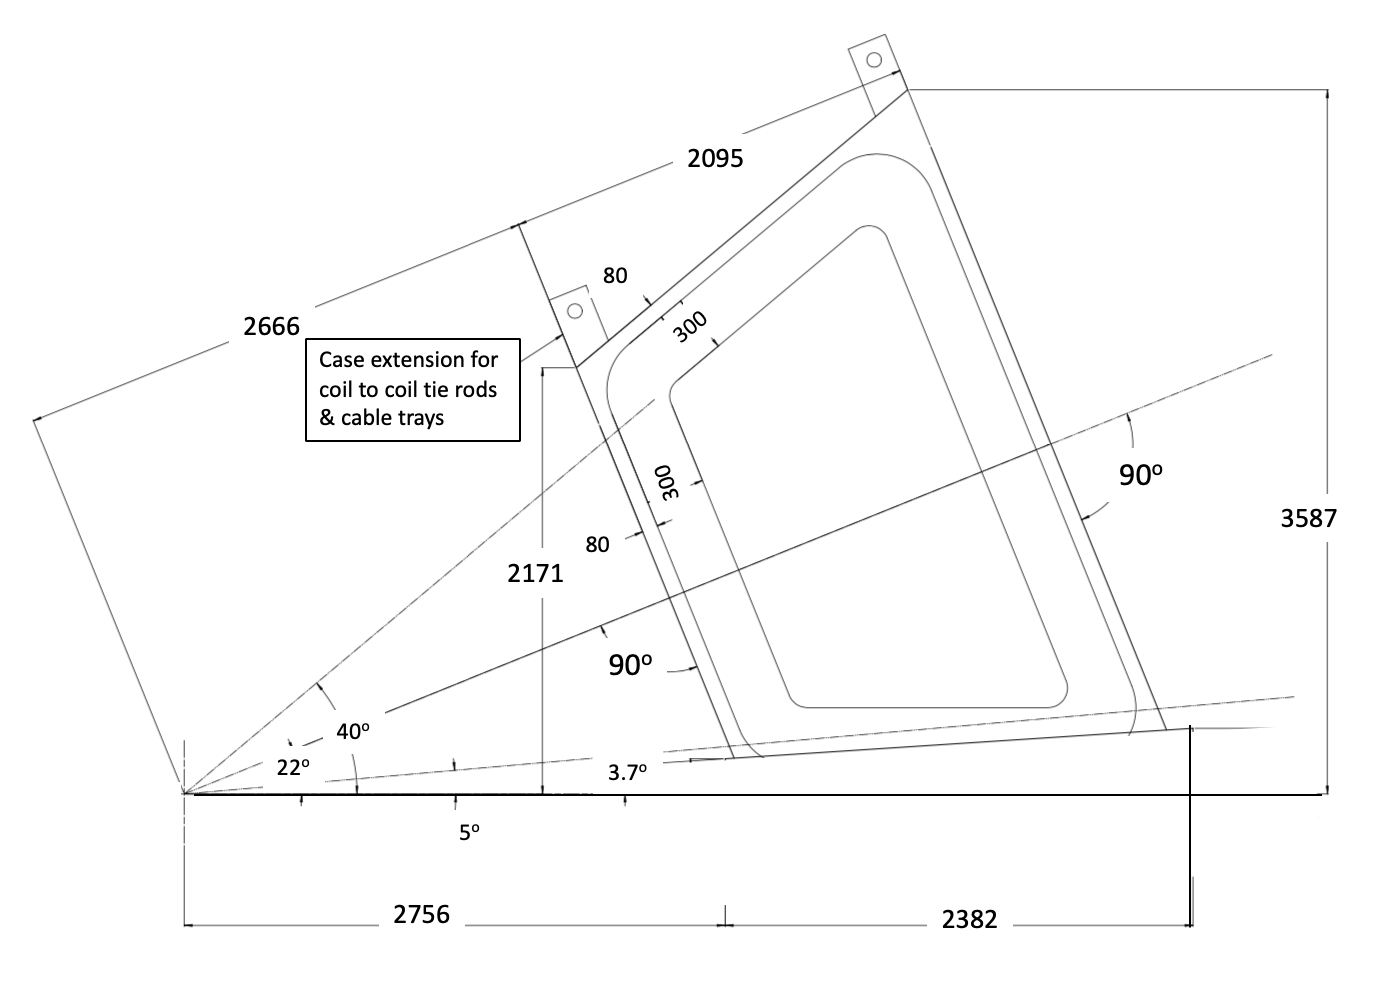
\includegraphics[width=1.70\columnwidth]{clas12_desired.png}}
\caption{The ideal shape and dimensions of one of the Torus magnet coils. All six coils are nominally identical to each
other, and are tilted forward at a $22.2^\circ$ angle relative to the vertical. The bores at the outer two corners
provide coil-to-coil connections.}
\label{coil-shape}
\end{figure*}


This paper provides a general description of the design, construction, and performance of CLAS12 and how it expands
upon the capabilities provided by the JLab 12~GeV energy upgrade. The CEBAF accelerator and experimental halls
are shown for the energy upgraded configuration in Fig.~\ref{cebaf12}. CEBAF is designed from two parallel linear
accelerators (linacs) based on superconducting radio frequency (RF) technology, and arranged in a race-track
configuration~\cite{Leemann:2001dg}. Spin-polarized electrons are generated in the gun, pre-accelerated in the
injector, and subsequently injected and accelerated in the north linac. They are then bent in a $180^\circ$ arc and
injected into the south linac. This is repeated four and a half more times to reach the final energy for Hall~D and up to
four times  for the desired delivery energies to Halls~A, B, and C. In the recirculating arcs, electrons are transported
in 5 independent out-of-phase tracks of different energies. For 12~GeV operation, five accelerating cryomodules with
four times higher gradients than were used in the 6~GeV CEBAF machine were added to each of the two existing linacs
to reach a maximum energy of 11~GeV for Halls~A, B, and C. One added arc path and one more pass through the north
linac were added to achieve the highest beam energy of 12~GeV for Hall~D. This highest beam energy is generated
exclusively for Hall~D, while the other three halls may receive beams at the same beam energy or at different beam
energies simultaneously, with up to a factor $10^5$ differences in current from 1~nA to 100~$\mu$A.

Major new detectors and other experimental equipment have been installed in Halls~B, C, and D that support a broad
science program of nuclear and hadronic physics. In Hall~D, a large hermetic detector with a solenoid magnet at its core
has been in operation since 2015. It incorporates tracking capabilities and photon detection over nearly the full $4\pi$
solid angle. This hall is dedicated to the production of mesons employing a linearly polarized photon beam. The new
CLAS12 spectrometer, displayed in a side view in Fig.~\ref{clas12} (from the design model) and in Fig.~\ref{clas12-photo}
(photograph), features large solid angle coverage and instantaneous luminosities of up to $\rm {10^{35}cm^{-2}s^{-1}}$ for
electron scattering experiments with multiple particle final states. 

Hall~C includes the new super-high momentum magnetic spectrometer (SHMS) in addition to the existing high momentum
spectrometer (HMS). In Hall~A, a new super big bite spectrometer (SBS) has been added to the existing high resolution 
spectrometer pair HRS$^2$, and other large installation experiments have been proposed. Complementing the new
equipment is the highly spin-polarized electron gun, high-power cryogenic targets, and several spin-polarized targets using
NH$_3$, ND$_3$, HD, $^3$He, and $^7$Li as target materials to support a broad range of polarization measurements.   

\begin{figure}[htbp!]
\centerline{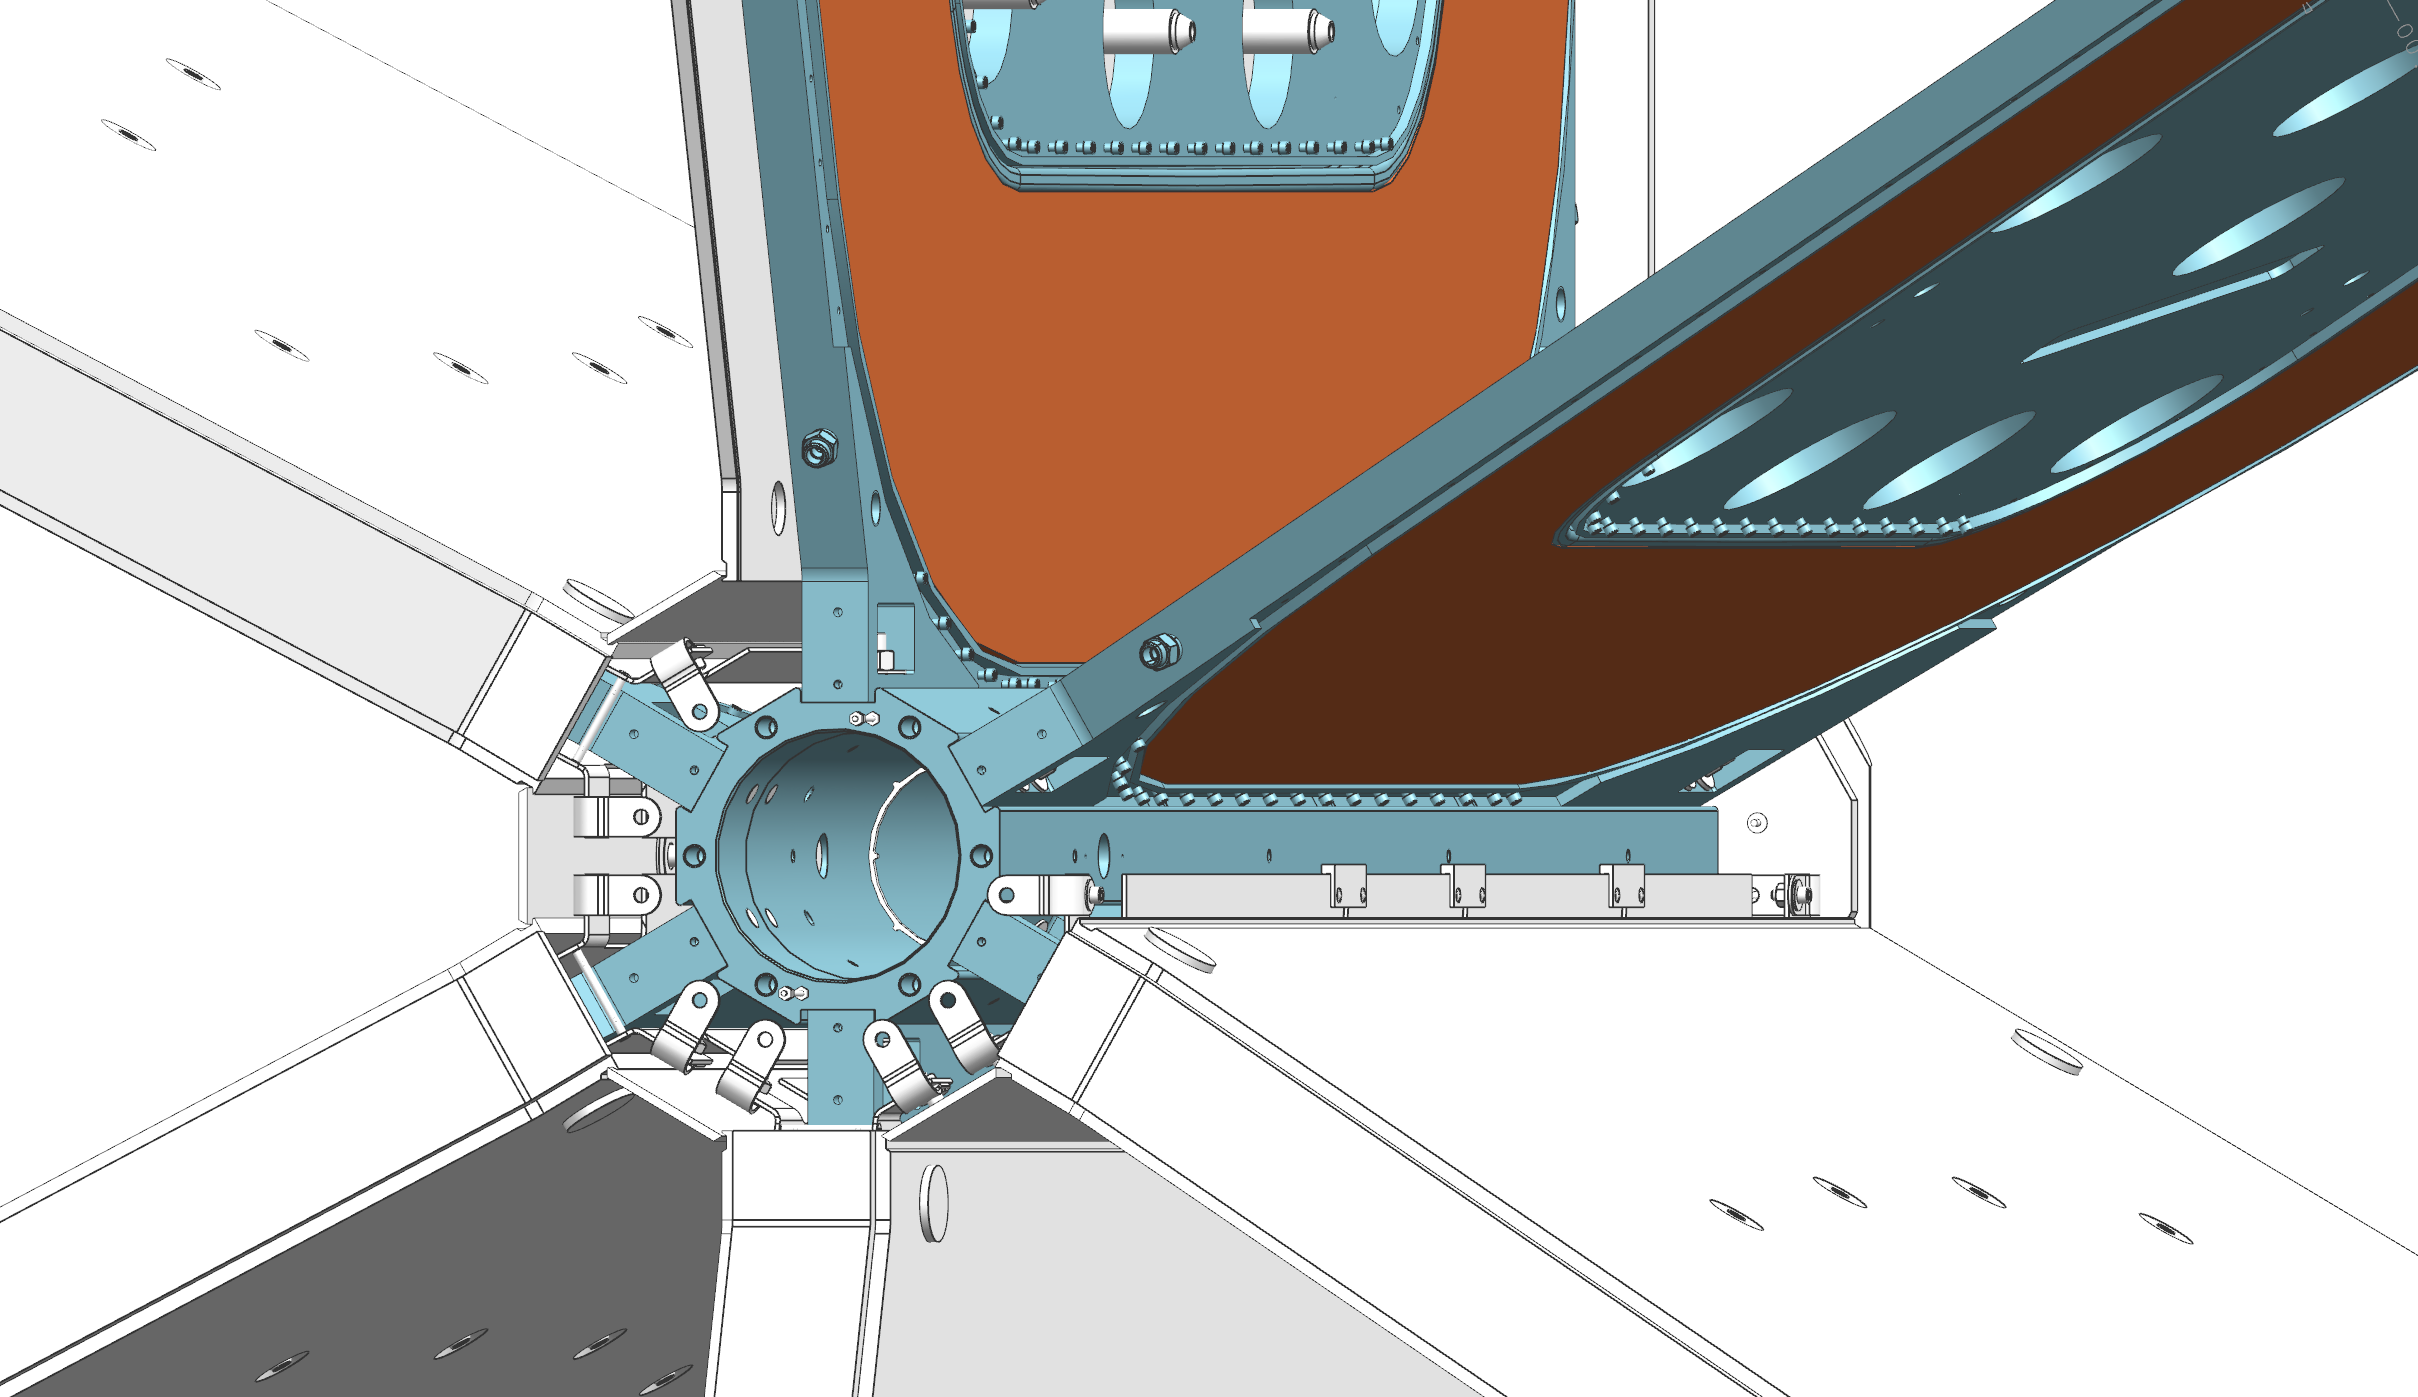
\includegraphics[width=1.00\columnwidth]{torus-hub-2.png}}
\caption{(Color Online) The six Torus coils are mounted on the cold central stainless steel cone that bears the centripetal force. The
dark-shaded areas indicate the location of the superconducting coils, surrounded by the cryostat and vacuum jacket.}
\label{coil-mount}
\end{figure}
\section{The CLAS12 System}

The design of CLAS12 is based on a combination of a toroidal magnetic field at polar angles up to $\approx 35^\circ$ and
a 5~T solenoidal field at central angles in the approximate polar angle range $35^\circ~\le \theta \le~125^\circ$. The
primary requirement driving this choice is the ability to measure charged particles at high momentum with good resolution
at forward angles, while operating the detector systems at high luminosity. This requires effective shielding of the
detector system from low energy electrons produced in the target material due to M\"oller scattering
$e^- + e^- \to e^- + e^-$ of the high-energy beam electrons on atomic electrons in the target material. The large majority
of those electrons are prevented from reaching sensitive detectors as they curl up in the strong longitudinal magnetic
solenoid field, and are then guided into a shielding pipe made from bulk tungsten material where they dump their energy. 

\subsection{The Torus Magnet}
\label{torus}
\begin{figure}[htbp!]
\centerline{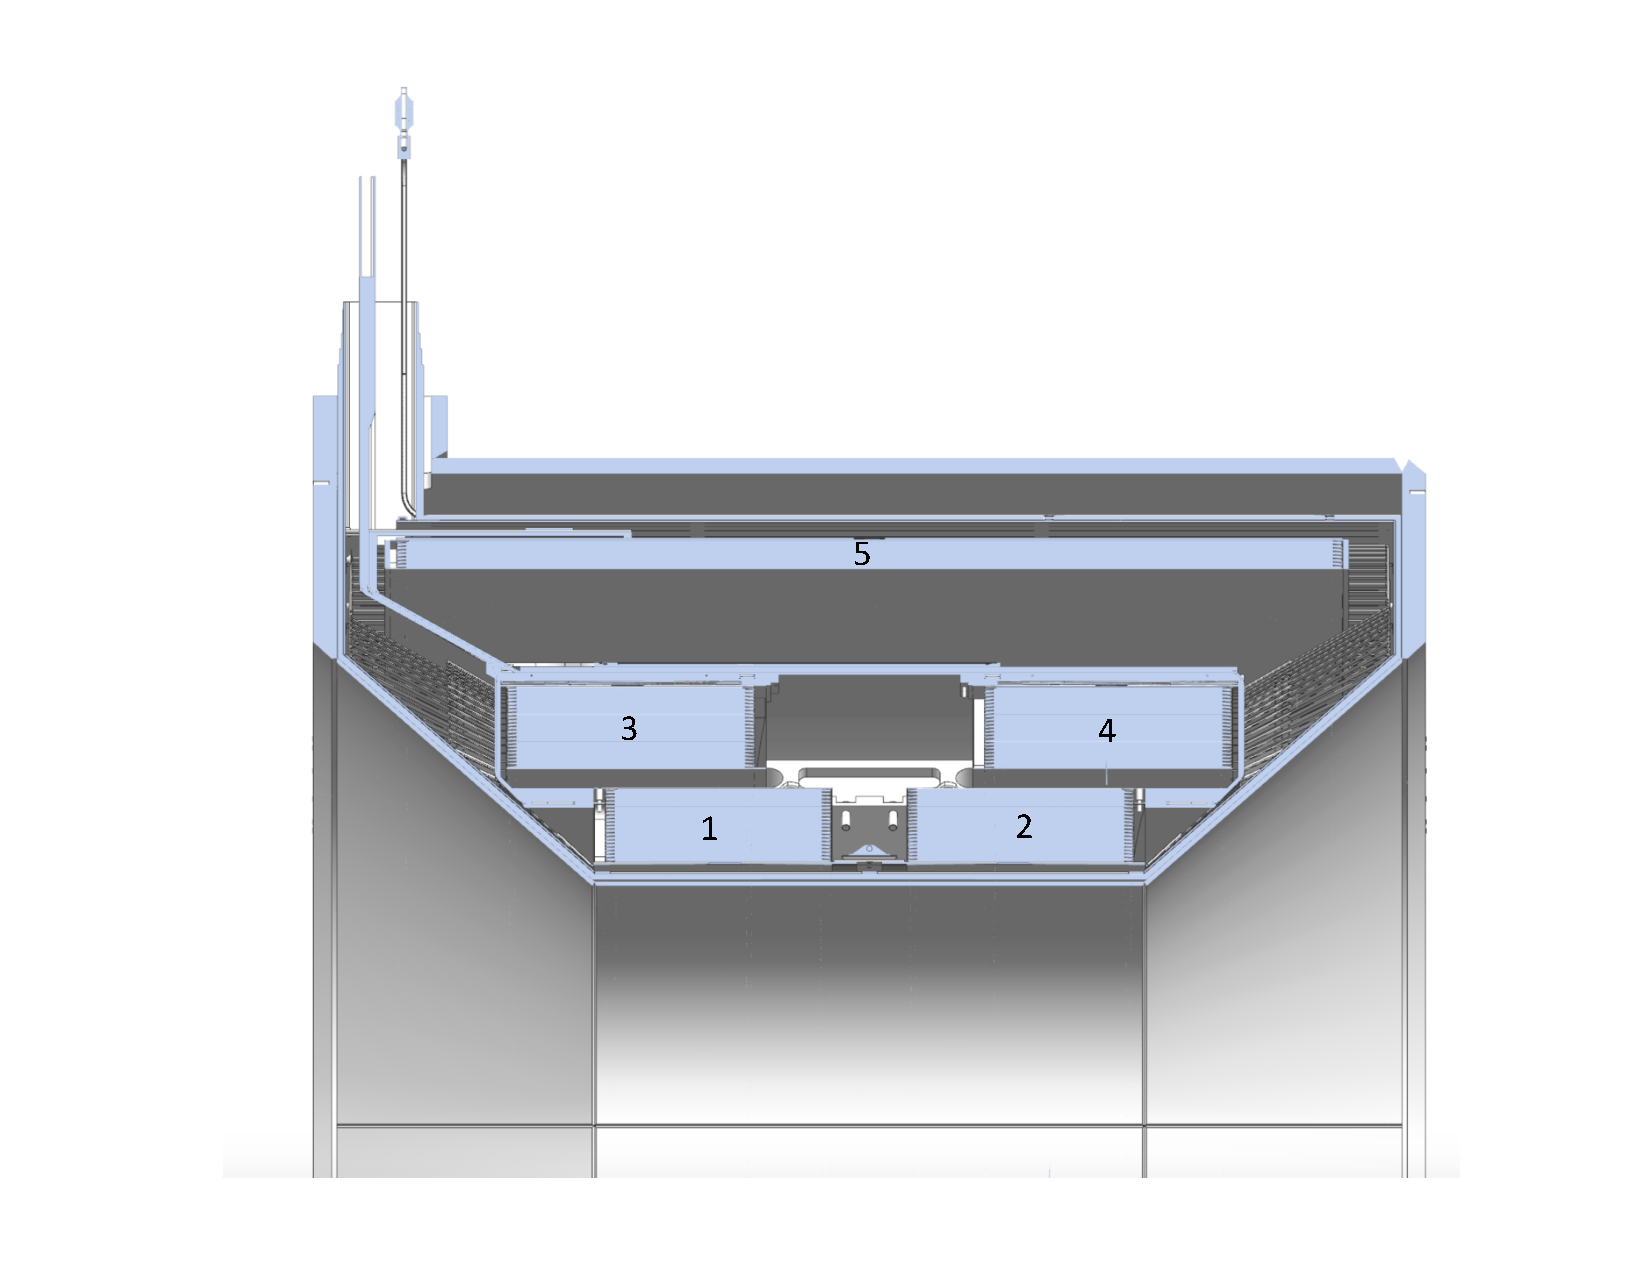
\includegraphics[width=1.3\columnwidth]{Solenoid.pdf}}
\caption{(Color Online) Cut view of the upper half of the solenoid coils with the 4 $2 \times 2$ main coils on the inside, and the shield
coil (5) on the outside. The shield coil provides effective compensation for the magnetic field sensitive photomultiplier 
tubes that are located just outside of the magnet cryostat (not shown). The nominal field in the center of the magnet is 5~T.}
\label{solenoid-coils}
\end{figure}
The contour of one of the six identical coils of the Torus magnet is shown in Fig.~\ref{coil-shape}. The geometrical
coverage as seen from the target ranges from $5^\circ$ to $40^\circ$ in polar angle. The symmetrically arranged six
magnet coils provide an approximate toroidal magnetic field around the beamline. The six coils are mounted in the
central cold hub on a common stainless steel cone, which also provides the geometrical symmetry for the alignment of
the coils near the magnet center (see Fig.~\ref{coil-mount}). This guarantees mounting of the coil packages in areas
where the magnetic field is expected to be maximal. A full view of the assembled Torus coils and cryostat is shown in
Fig.~\ref{clas12-magnets}(left). The coverage in azimuthal angle depends on the polar angle of the particle trajectory,
and ranges from 50\% of $2\pi$ at $5^\circ$ to about 90\% of $2\pi$ at $40^\circ$.


Each superconducting coil is made from a double-pancake potted in an aluminum case. The number of windings per
pancake is 117. The conductor is SSC outer dipole cable soldered into a 20~mm $\times$ 2.5~mm copper channel with
a turn-to-turn insulation of 75~$\mu$m fiber-glass tape. Operating at a nominal current of 3770~A, the peak field is
3.58~T at the inner turns close to the warm bore. For symmetry reasons the field on the beam axis is ideally equal to
zero, with a small remnant field present due to imperfections in the magnet assembly and coil positions. The $\int {Bdl}$
at the nominal current is 2.78~Tm at $5^\circ$ and 0.54~Tm at $40^\circ$. The inductance of the magnet is 2.0~H
and the stored energy 14.2~MJ. The magnet has liquid-N$_2$ cooled heat shields. After assembly and cool down,
the magnet reached full field immediately. For details on the design and operation of the Torus magnet, see
Ref.~\cite{clas12-magnets}.
\begin{figure*}[htbp!]
\hspace{-0.5cm}\centerline{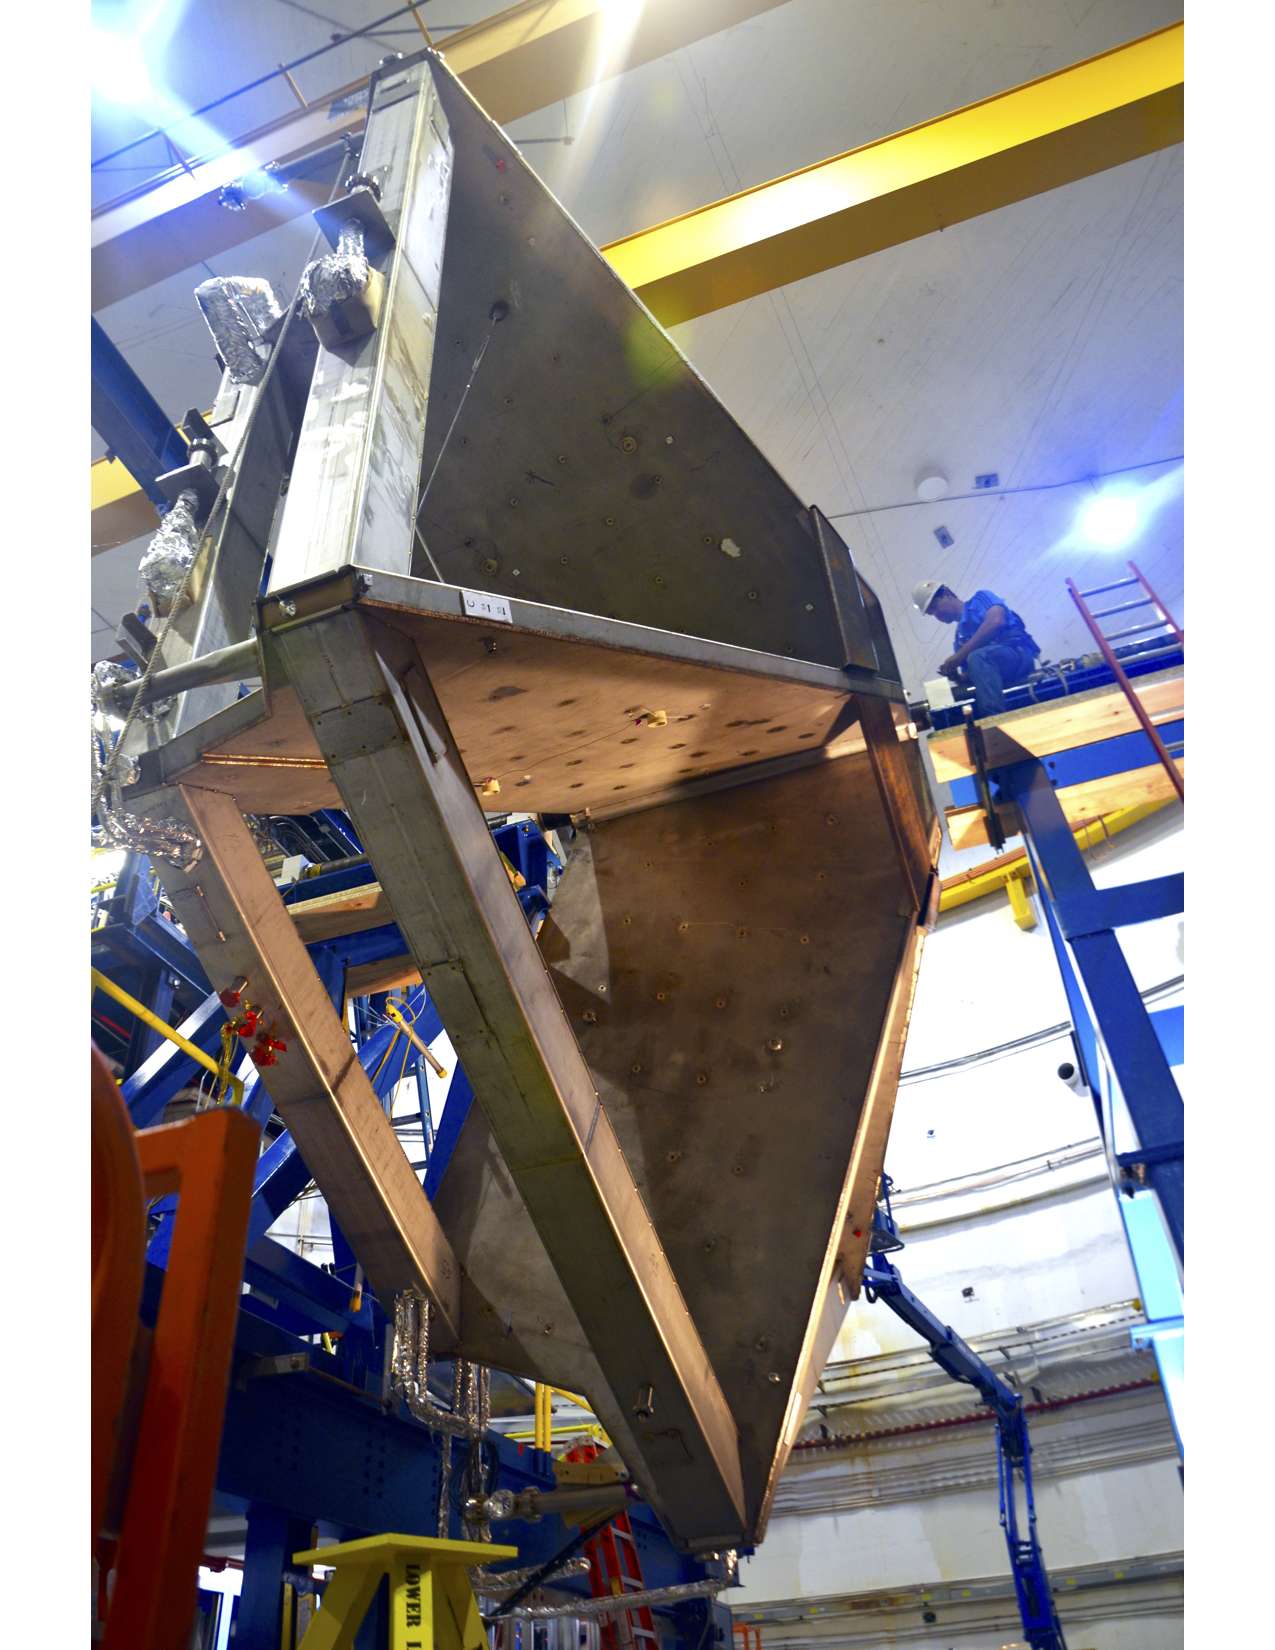
\includegraphics[width=1.23\columnwidth]{Torus-assembled.pdf}
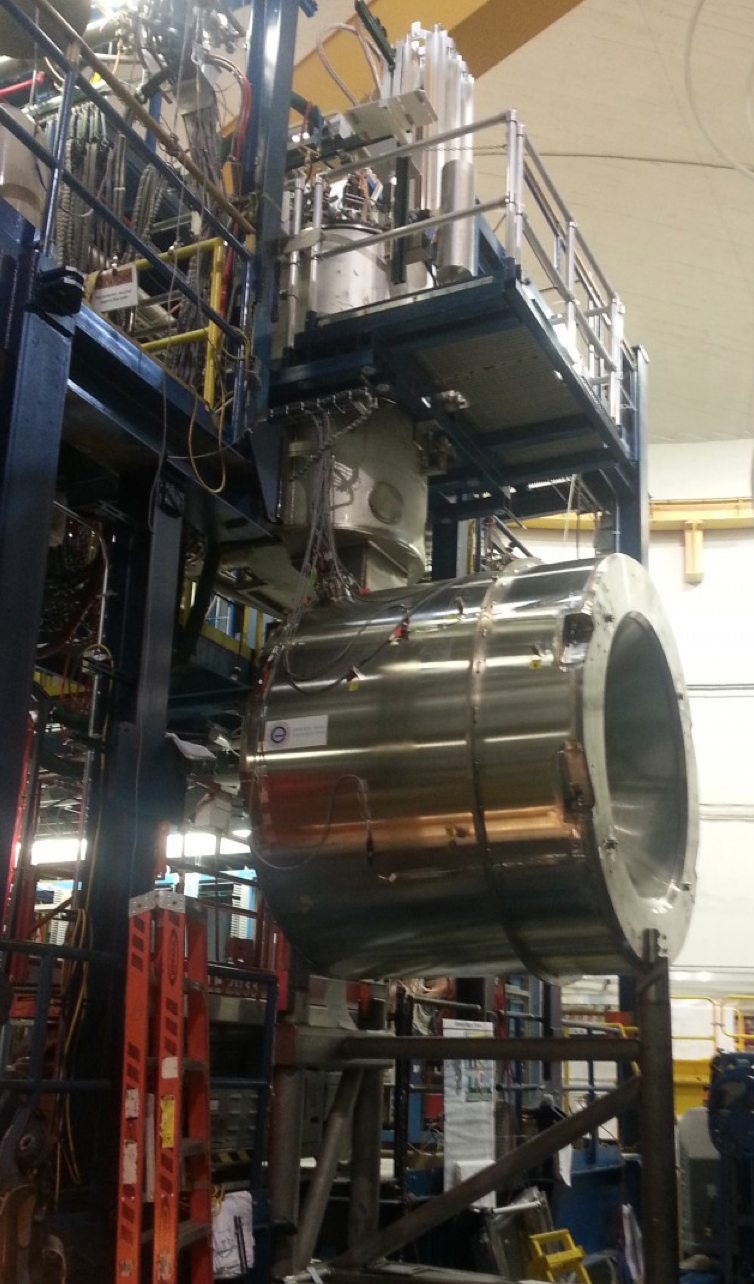
\includegraphics[width=0.94\columnwidth]{solenoid-magnet.png}}
\caption{(Color Online) The CLAS12 magnet system. Left: The Torus magnet with all six coils mechanically assembled in the common 
cryostat. The coil cryostat, which is fabricated from non-magnetic steel, has an outside width of 124~mm. The cross
bars provide a cold (5~K) cryogenic connection of neighboring coils, and counteract the out-of-plane forces to provide
mechanical stability to the full magnet. Due to the large physical size of the assembled Torus magnet, the final assembly
of the magnet had to be completed in Hall~B. Right: The fully assembled Solenoid magnet including all cryogenic
connections on the beamline at the beginning of cool down, before the detector installation.}
\label{clas12-magnets}
\end{figure*}

\subsection{The Solenoid Magnet}

The Solenoid magnet is a self-shielded superconducting magnet around the beamline used to generate a field primarily
in the beam direction. Fig.~\ref{solenoid-coils} shows the design layout of the solenoid coils, and the fully assembled
magnet is shown in Fig.~\ref{clas12-magnets} (right). The design is driven by the physics requirements to (a) provide
a magnetic field for particle tracking at large angles, (b) act as a M\"oller electron shield, and (c) provide a highly
uniform field at the magnet center for the operation of dynamically polarized proton and deuteron targets.
\begin{figure}[htbp!]
\centerline{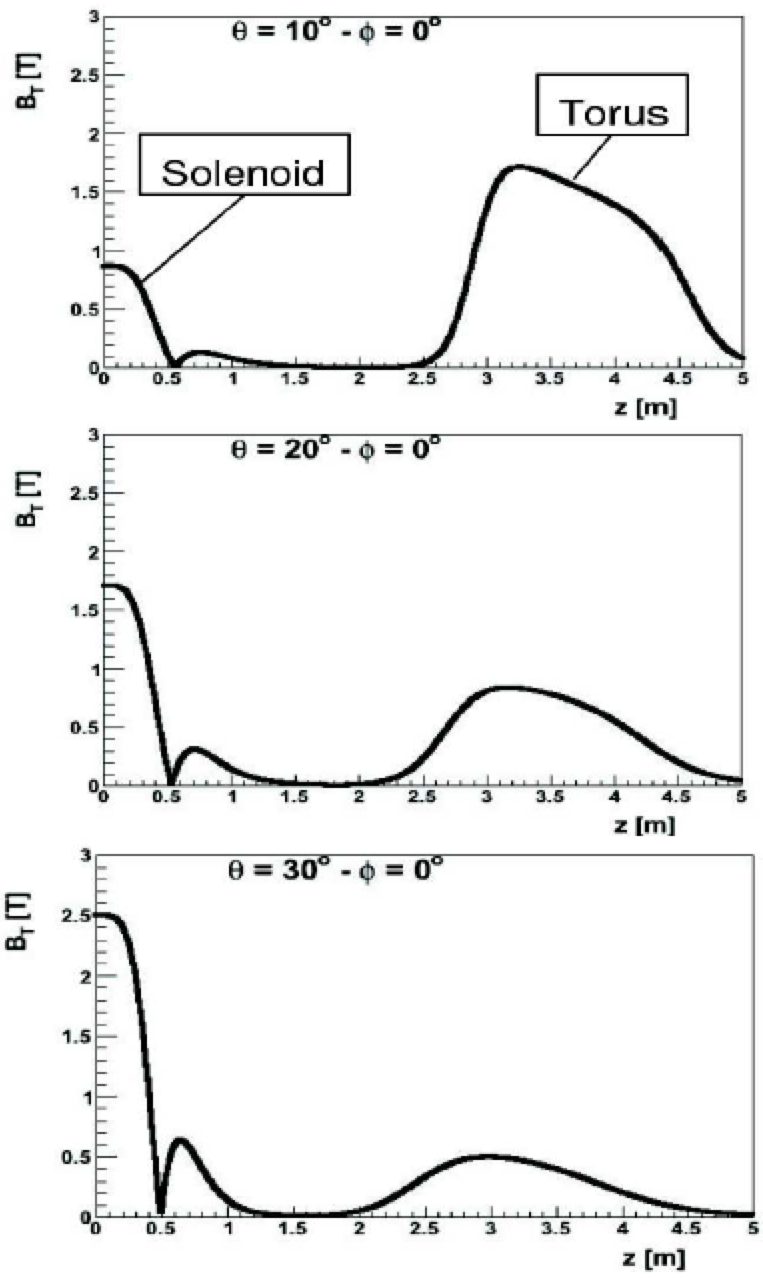
\includegraphics[width=0.65\columnwidth]{magfield.png}}
\caption{Combined Solenoid and Torus magnetic fields, showing the total transverse magnetic field along the radial
distance from the Solenoid center. The two magnetic fields act differently on charged particles. Only the transverse
components act on the charged tracks. Their effect depends on the orientation of the field relative to the momentum
vector of the charged particle.} 
\label{solenoid-torus}
%\end{figure}
%\begin{figure}[htbp!]
\vspace{0.5cm}
\centerline{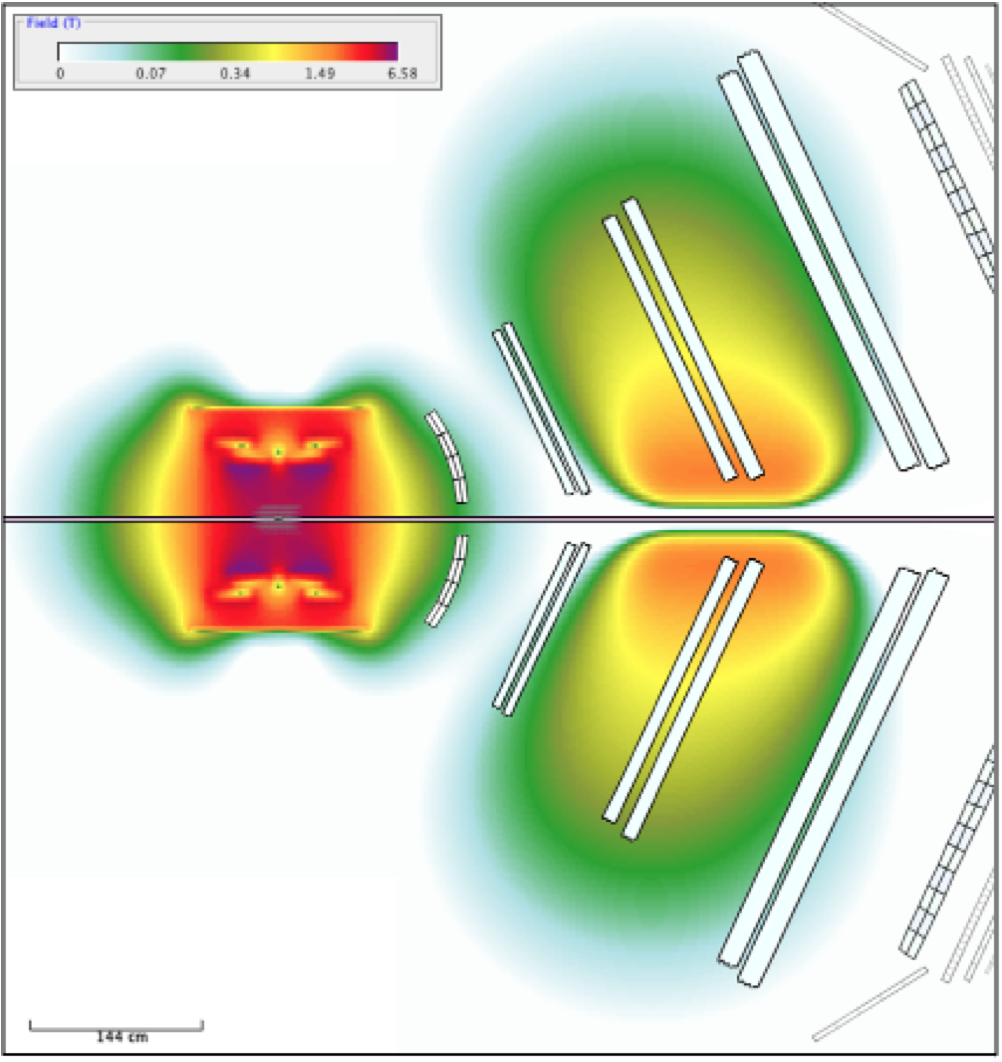
\includegraphics[width=0.8\columnwidth]{magfield-2.png}}
\caption{(Color Online) Combined Solenoid and Torus magnetic stray fields with both magnets at full current. The 
color code shows the total magnetic field of both Solenoid and Torus at full current. The open boxes indicate the 
locations and dimensions of the active detector elements. The two field volumes have very little overlap.
The Solenoid field is radially largely contained due to 
the shielding coil. The Torus field is radially widely spread out due to the very open geometry of the Torus coils.  }
\label{stray-field}
\end{figure}
The magnet consists of 4 cylindrical coils arranged in two packages at different radial distances to the beamline. The
fifth coil is located outside of the 4 inner coils and generates a magnetic field that compensates the field of the 4 inner
coils and thus acts as an active magnetic shield. The number of turns in the main coils is 3704
$(2 \times 840 + 2 \times 1012)$, and in the shield coil 1392. The magnet is powered at a nominal currents of 2416~A.
The integrated field length along the magnet center is $\int Bdl = 7.0$~Tm, generating a stored energy of 20~MJ. At
full current the solenoid generates a 5~T magnetic field at its center. The magnet has an inner warm bore of 78~cm
diameter where all the central detectors are placed.  For details on the design and operation of the Solenoid magnet,
see Ref.~\cite{clas12-magnets}.

The distribution of the absolute magnetic field along lines of constant polar angles seen from the target position is shown
in Fig.~\ref{solenoid-torus}. Both the Torus and Solenoid magnetic fields are included. The stray field of the Solenoid
magnet and of the Torus magnet alone is shown in Fig.~\ref{stray-field}.  


%\begin{figure}[htbp!]
%\centerline{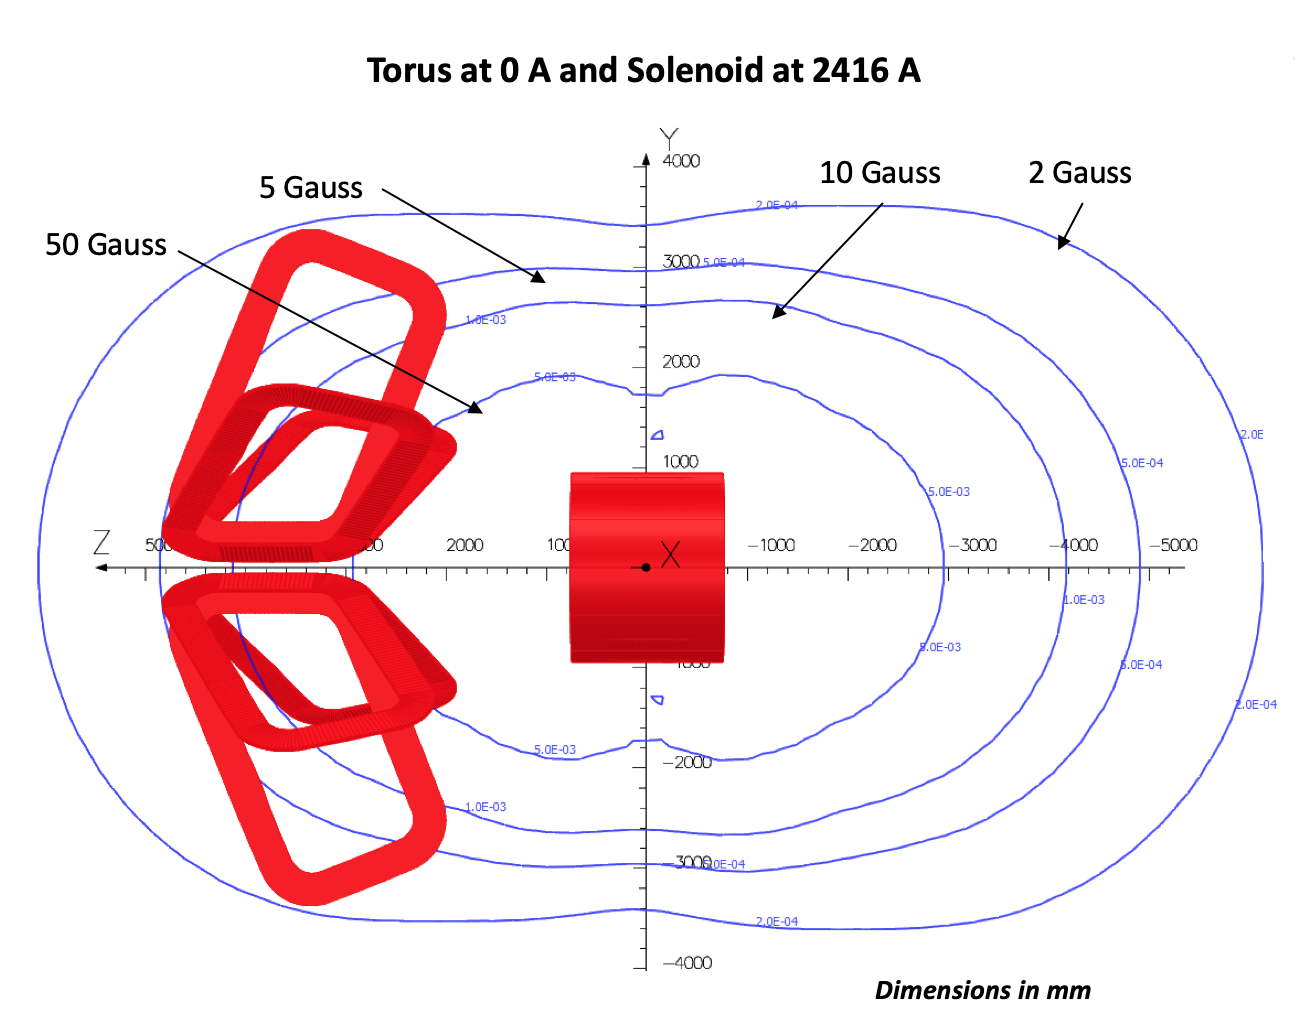
\includegraphics[width=1.0\columnwidth]{mag-field-1.png}}
%\caption{(Color Online) Solenoid magnetic stray fields with the magnet at full current and the Torus off. }}
%\label{stray-field1}
%\end{figure}


\begin{figure}[ht]
\centerline{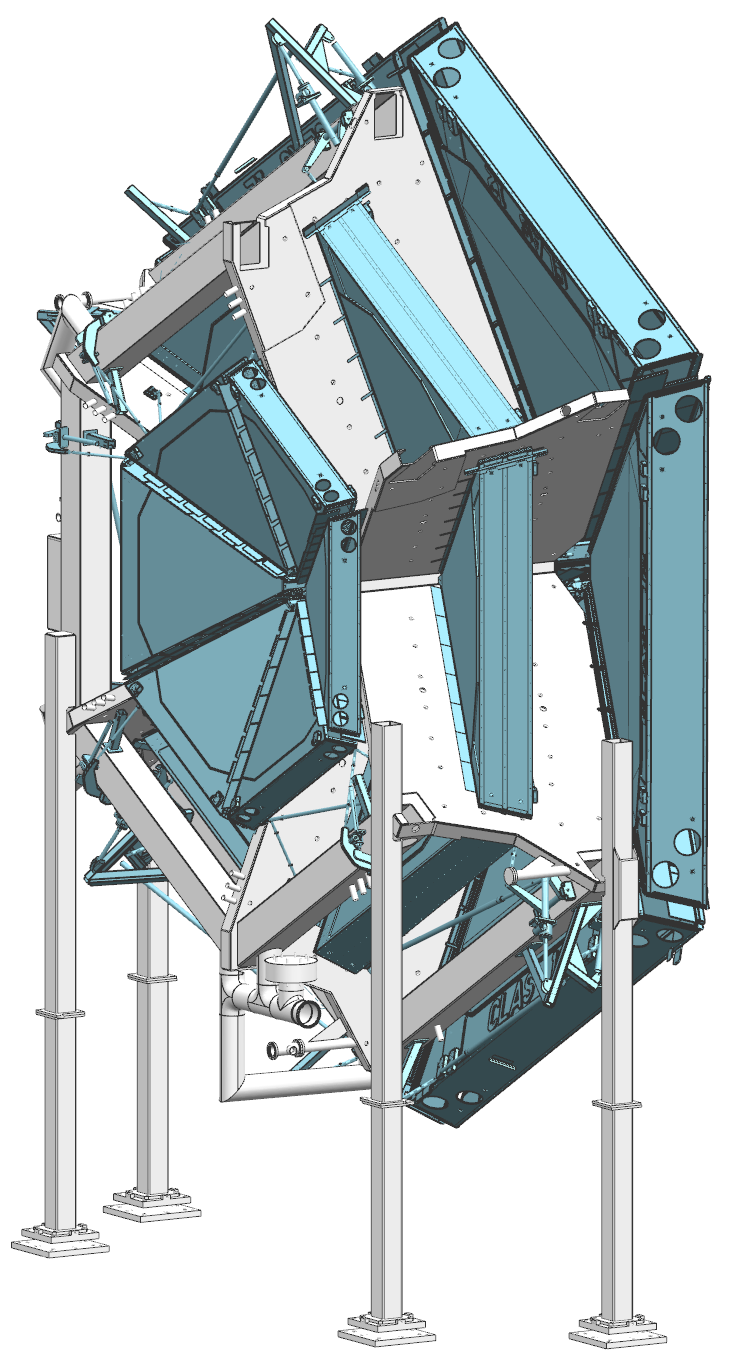
\includegraphics[width=0.60\columnwidth]{dc-view-4.png}}
\caption{(Color Online) Drift chamber system in the CLAS12 forward tracking system from the design model. 
The R1 chambers (blue shades) are located just in front of the Torus magnet coils (gray shade). 
The R2 chambers are sandwiched between the coils 
of the magnet, and the R3 chamber are located just downstream of the magnet.}
\label{clas12-dc}
\end{figure}

\begin{figure*}[htbp!]
\centerline{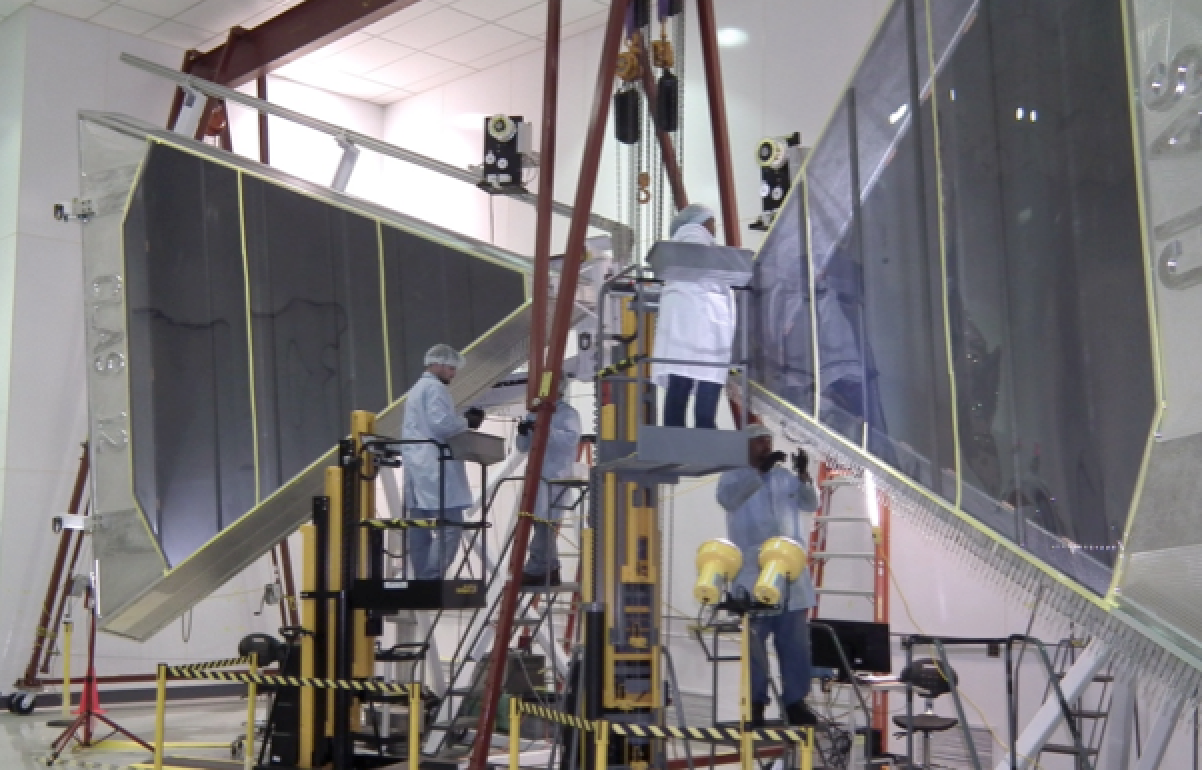
\includegraphics[width=1.65\columnwidth]{DC-R3.png}}
\caption{(Color Online) Wire stringing of two R3 chambers in the Jefferson Lab clean room.}
\label{dc-stringing}
\end{figure*}

\subsection{The CLAS12 Forward Detector (FD)}

The Forward Detector has at its core a six-coil superconducting Torus magnet with the individual coils
symmetrically arranged around the beamline within a circle of approximately 7.2~m in diameter. The six coils of the
Torus magnet mechanically support the forward tracking system, which consists of independent drift chambers in
each of the six sectors of the Torus magnet. Each of the six drift chamber sectors has a total of of 36 layers with
112 sense wires, arranged in 3 regions (R1, R2, and R3) of 12 layers each. In each of the six Torus sectors the drift
chambers are arranged identically. As displayed in Fig.~\ref{clas12-dc}, the R1 chambers are located at the entrance
to the Torus magnetic field region, the R2 chambers are located inside the magnet where the magnetic field is close
to its maximum, and the R3 chambers are placed in a low magnetic field space just downstream of the Torus magnet.
This arrangement provides independent and redundant tracking in each of the six Torus sectors. Each of the 3 regions
consists of 6 layers with wires strung at $\Delta{\phi} = 84^\circ$ from the sector mid-plane and 6 layers with wires
strung at $\Delta{\phi} = 96^\circ$ from sector mid-plane. This stereo view enables excellent resolution in the most
important polar angle (laboratory scattering angle), and good resolution in the less critical azimuthal scattering angle.
Figure~\ref{dc-stringing} shows the wire stringing operation for the large R3 chambers. For details of the DC
construction and performance, see Ref.~\cite{DC}.




\subsection{Particle Identification After Tracking}

Cherenkov counters, time-of-flight detectors, and electromagnetic calorimeters are located downstream of the
tracking system to provide particle identification and energy measurements for electrons, high energy photons,
and neutrons.  

%Figure~\ref{clas12-fd} shows a beam's eye view of the assembled FD, with the six Torus coil
%cryostats symmetrically arranged around the beamline. It should be noted that the entire Torus magnet is placed
%in one hermetic vacuum system, with the coil cooling provided by cooling tubes soldered to the inner side of the coils.  
%In the following we briefly describe the CLAS12 FD systems used for particle identification. 

%\begin{figure}[htbp!]
%\centerline{\includegraphics[width=0.9\columnwidth]{clas12-fd.png}}
%\caption{(Color Online) Forward Detector as seen from the beamline before the installation of the drift chamber tracking system.
%The six structures extending radially from the apex are the cryostats of the individual Torus magnet coils. The steel
%cross bars in the middle of the sectors supported the coils during magnet assembly, and were removed before operation.
%When energized the magnetic field lines loop around the azimuth, falling in strength approximately as the inverse of
%the radial distance from the magnet center.  {\bf FIND PHOTO WITH BETTER LIGHTING}}
%\label{clas12-fd}
%\end{figure}

\begin{figure}[htbp!]
\centerline{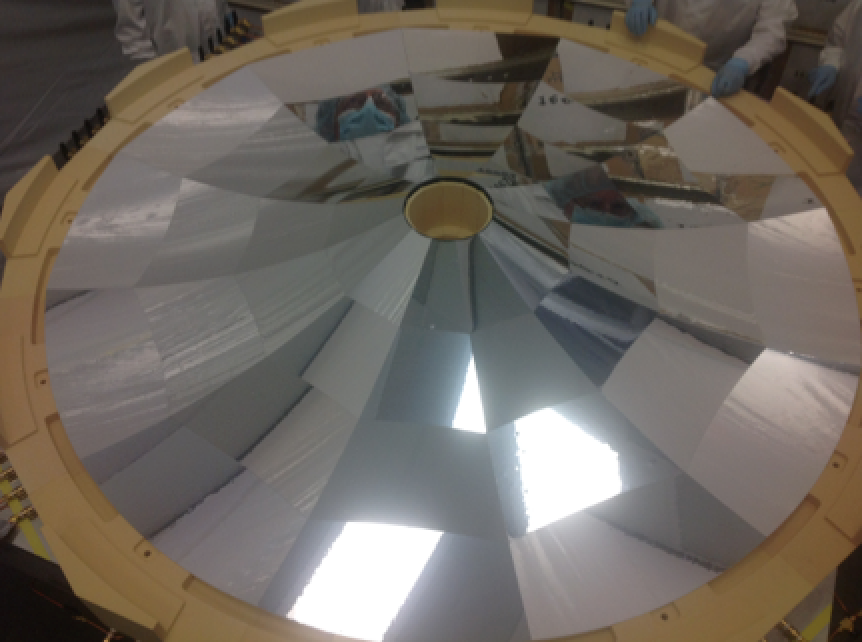
\includegraphics[angle=90,width=0.75\columnwidth]{HTCC-mirror.png}}
\caption{The HTCC mirror with its 48 mirror facets, each reflecting the Cherenkov light to a different photomultiplier
tube. The mirror spans about 2.4~m in diameter.}
\label{htcc}
%\end{figure}
%\begin{figure}[htbp!]
\centerline{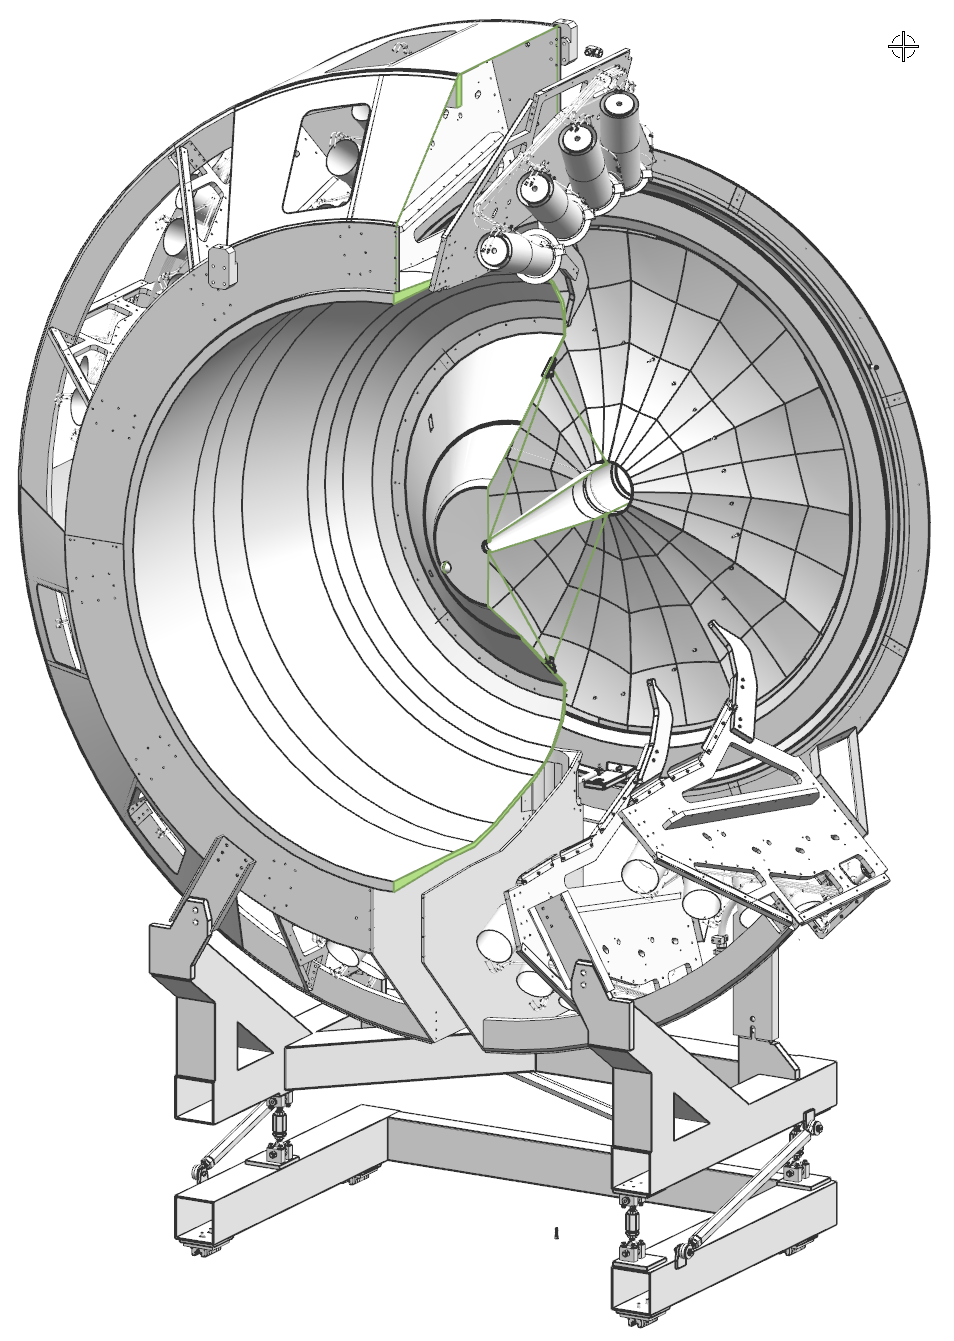
\includegraphics[width=0.9\columnwidth]{htcc-view-3.png}}
\caption{Cut view of the assembled HTCC detector. The container spans about 4.5~m in diameter. The mirror is
seen at the downstream end to the right. The phototubes are mounted in 12 sectors and in groups of 4 at the outer
perimeter of the container. Light collection uses additional Winston cones and 5~in photomultiplier tubes.}
\label{HTCC-container}
\end{figure}

\subsection{High Threshold Cherenkov Counter (HTCC)}


The HTCC is the main detector to separate electrons (positrons) with momenta below 4.9~GeV from charged pions,
kaons and protons. The detector has full coverage of 360$^\circ$ in azimuth and spans from 5$^\circ$ to 35$^\circ$
in polar angles. It has no blind areas in its complete solid angle coverage. The detector is located downstream of the
production target, sandwiched between the Solenoid magnet and the Torus magnet, in front of the forward tracking
detectors. 

The HTCC system is required to provide high rejection of charged pions and low background noise for reliable 
identification of scattered electrons in a dense electromagnetic background environment. The HTCC is a single unit
operated in dry CO$_2$ gas at 1~atm pressure. It is constructed using a multi-focal mirror of 48 elliptical mirror
facets that focus the Cherenkov light on 48 phototubes with quartz windows of 125-mm diameter. The phototubes
are located in a magnetic field of up to 35~G oriented along the phototube axes and are covered with a multi-layer
magnetic shield and active compensation coils. In order to minimize multiple scattering in the HTCC detector materials,
e.g. the mirror system with its backing structure, and to limit its impact on the momentum analysis of charged tracks in
the Torus field, the HTCC mirror system is constructed using a backing structure of low-density composite material. 
The amount of solid material seen by charged particles passing through the HTCC volume is 135~mg/cm$^2$. 

The HTCC is also used to generate a fast signal to be used as a trigger for scattered electrons. The HTCC operates
in conjunction with energy deposited in the electromagnetic calorimeters to identify electrons of specific energies.
The $360^\circ$ mirror system of the HTCC is shown in Fig.~\ref{htcc}. Figure~\ref{HTCC-container} shows a cut view
of the assembled HTCC detector. For details of the HTCC construction and performance, see Ref.~\cite{HTCC}.   


\subsection{Low Threshold Cherenkov Counters (LTCC)}

The LTCC system is part of the CLAS12  Forward Detector and is used for charged pion and kaon discrimination at
momenta greater than 3.5~GeV. The LTCC system consists of boxes shaped like truncated pyramids. Four of the six
sectors of CLAS12 are equipped with one LTCC box. Each LTCC box contains 108 light-weight mirrors with composite
backing structure, 36 Winston light-collecting cones , 36 125~mm diameter photomultiplier tubes, and 36 magnetic
shields. The LTCC boxes are filled with heavy $\rm C_4F_{10}$ radiator gas, providing pion discrimination from kaons
for momenta of 3.5 to 9~GeV.  The LTCC system has previously been used to detect electrons in the CLAS detector at
lower energies~\cite{Adams:2001kk}. It has been refurbished to provide higher efficiency for charged pion detection
by increasing the volume of the radiator gas, refurbishing the elliptical and hyperbolic mirrors with new coating, and
improving the sensitivity of the phototubes to Cherenkov light by coating their entrance windows with wavelength
shifting material that absorbs UV light at wavelength below 300~nm and re-emits two back-to-back photons at larger
wavelength. The components of the LTCC optical mirror system and its arrangement are shown in Figs.~\ref{ltcc1}
and \ref{ltcc2}.  For details of the LTCC construction, the detector refurbishments, and its performance, see
Ref.~\cite{LTCC}.   

\begin{figure*}[htbp!]
\centerline{\includegraphics[width=1.6\columnwidth]{ltccArray.png}}
\caption{(Color Online) Layout and components of the optical mirror system within each LTCC box from the design model.}
\label{ltcc1}
\end{figure*}
\begin{figure}[htbp!]
\centerline{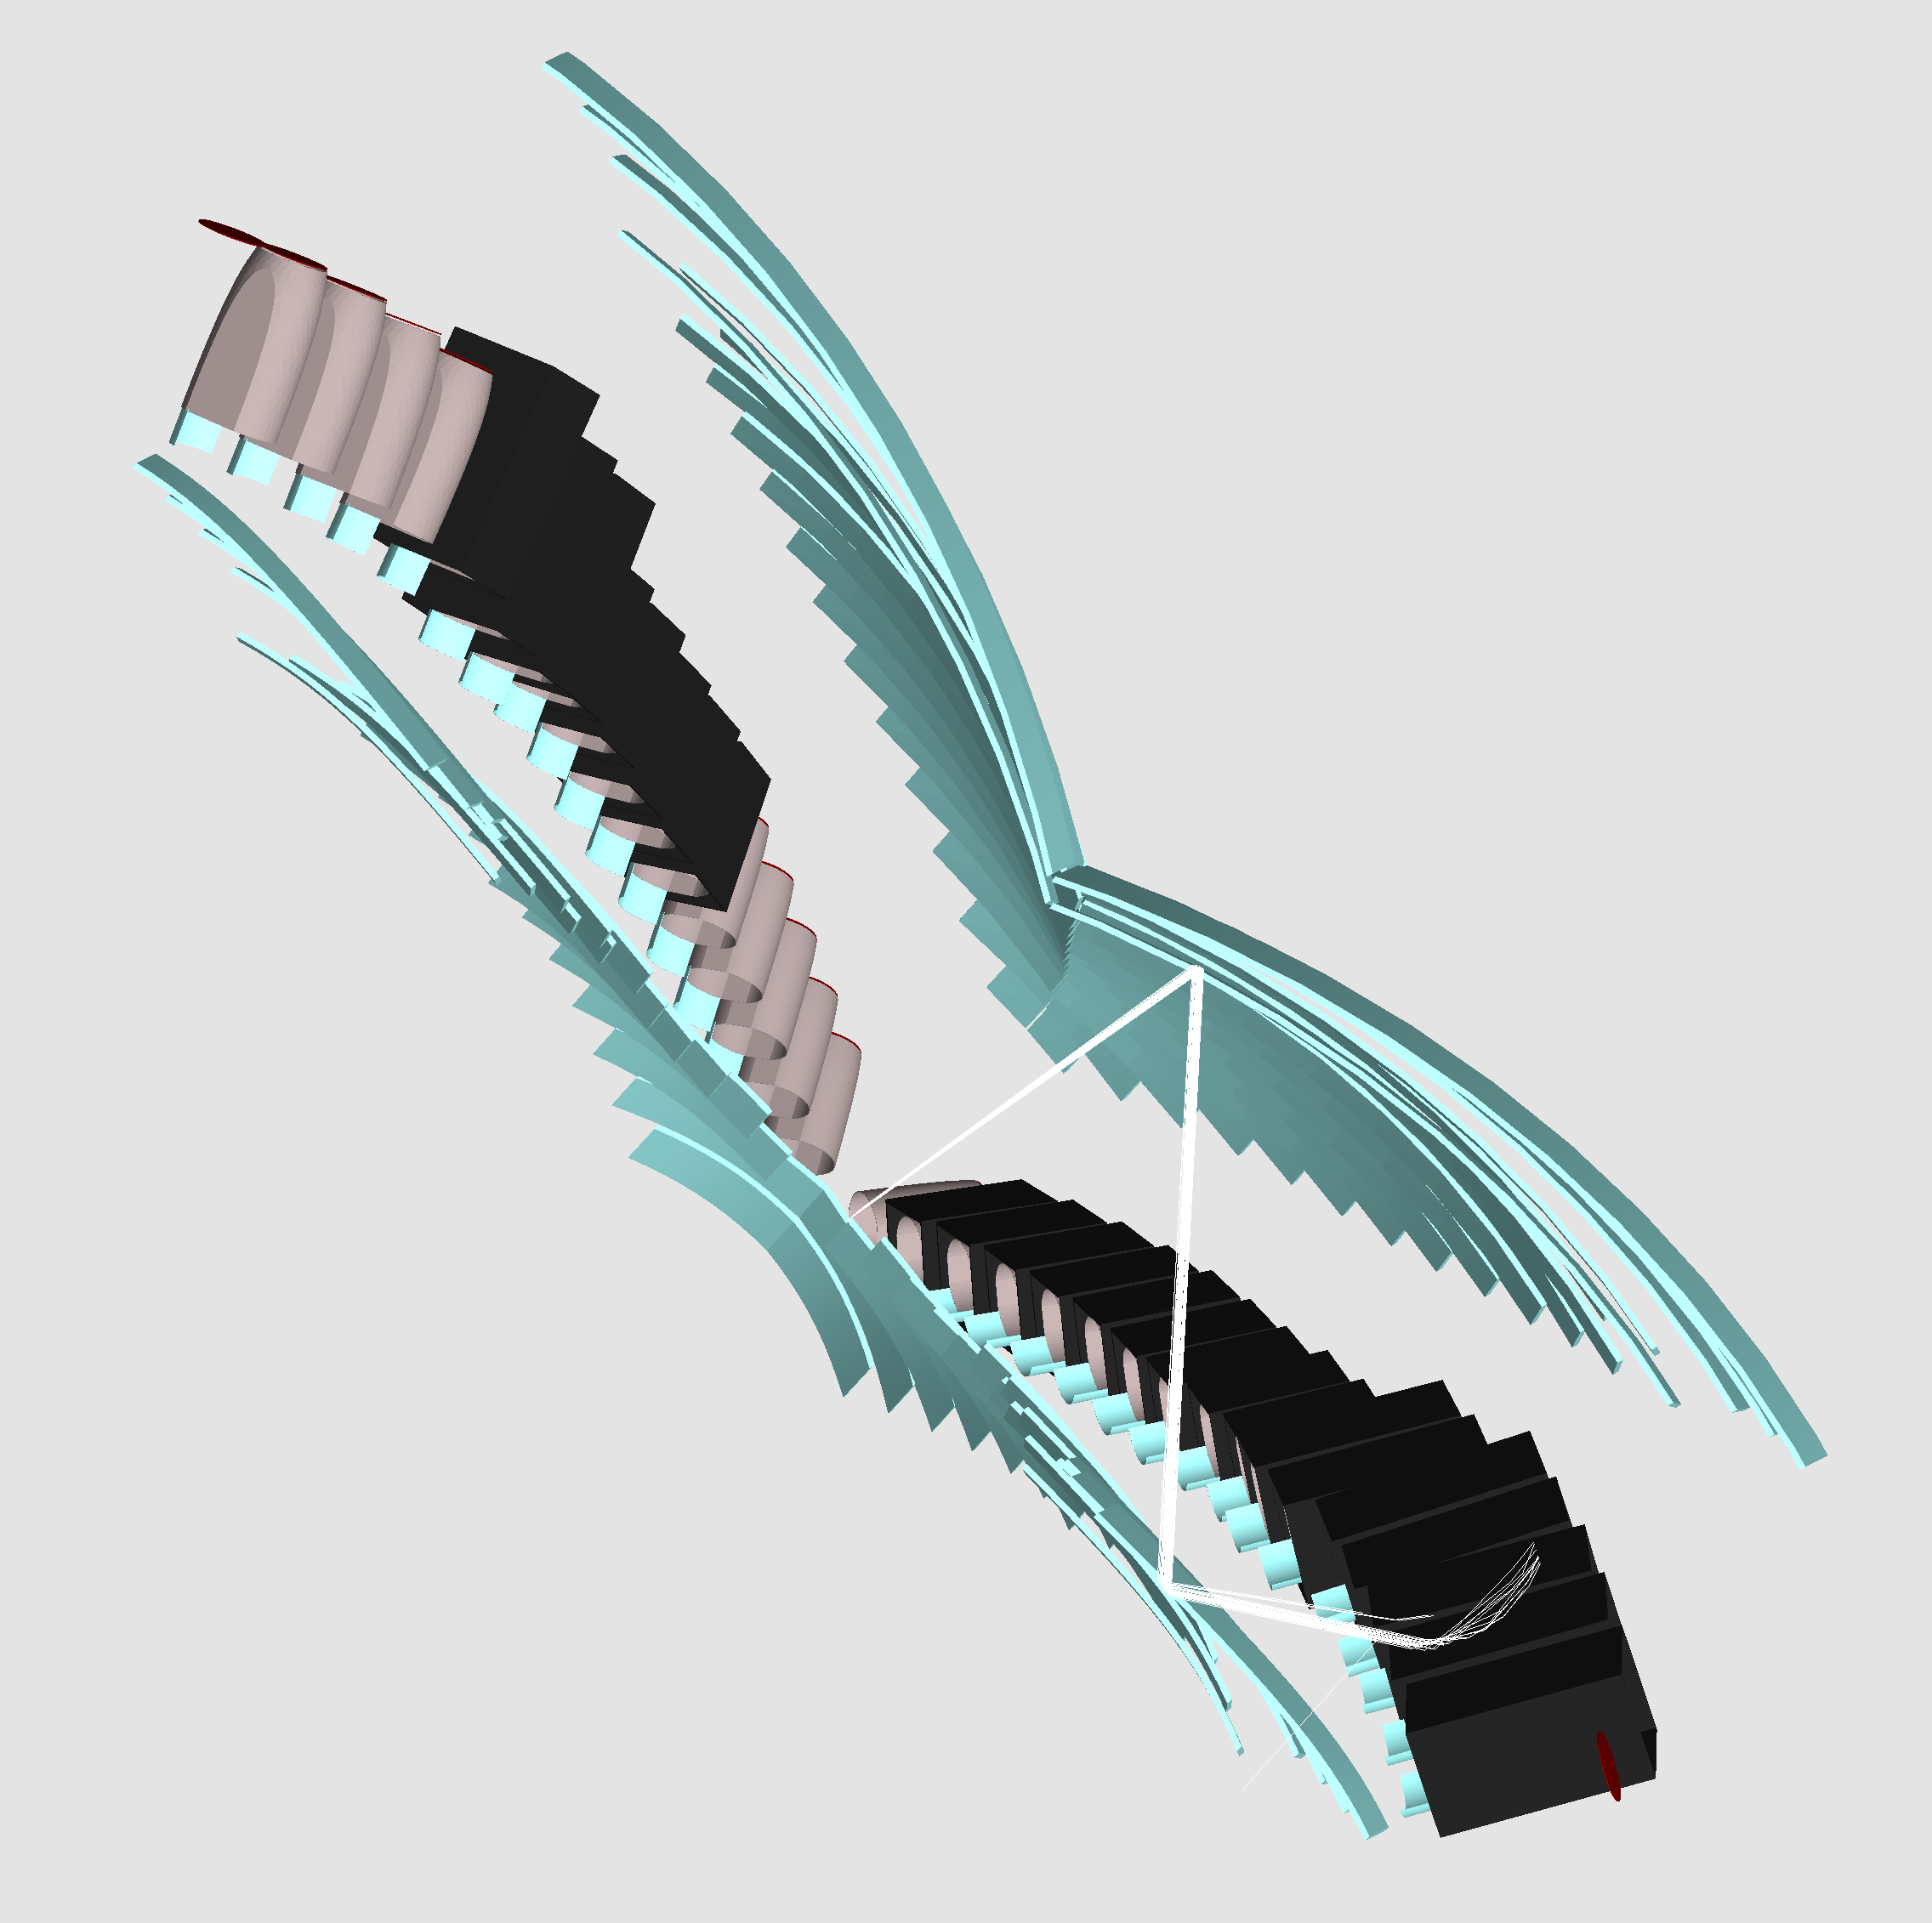
\includegraphics[width=1.0\columnwidth]{ltcc-mod6.png}}
\caption{(Color Online) Perspective representation of the LTCC optical system. A charged particle enters from the left-bottom and
generates Cherenkov light in the radiator gas volume. The light is reflected off the elliptical mirror array towards the
hyperbolic mirror array, from where it is reflected towards the Winston cone and 5-in photomultiplier. The large
acceptance coverage requires a complex mirror system for efficient light collection. }
\label{ltcc2}
\end{figure}

\subsection{Ring Imaging Cherenkov Detector (RICH)} 

Some experiments require the detection and identification of charged kaons in momentum ranges that are not 
accessible with the standard time-flight method used with the FTOF scintillators, or with the LTCC Cherenkov
counters. The time-of-flight resolution of the scintillators is no longer sufficient, and the momentum threshold of the LTCC
is too high to detect and separate kaons from protons in the momentum range from 3 to 8~GeV. For that purpose
an additional RICH detector was built and incorporated in one of the CLAS12 sectors to replace the corresponding
LTCC sector. The RICH detector is designed to improve CLAS12 particle identification in the momentum range
3-8~GeV. It incorporates aerogel radiators, visible light photon detectors, and a focusing mirror system that is
used to reduce the detection area instrumented by photon detectors to 1~m$^2$.  Multi-anode photomultiplier
tubes (MA-PMTs) provide the required spatial resolution and match the aerogel Cherenkov light spectrum in the
visible and near-UV region. For forward scattered particles ($\theta < 13^\circ$) with momenta 3 - 8~GeV, a
proximity imaging method with thin (2~cm) aerogel and direct Cherenkov light detection is used. For larger incident
particle angles of $13^\circ < \theta < 25^\circ$ and momenta of 3 - 6~GeV, the Cherenkov light is produced by a
thicker aerogel layer of 6~cm, focused by a spherical mirror, and undergoes two further passes through the
thin radiator material and a reflection from planar mirrors before detection. Figure~\ref{RICH} shows the RICH mirror
system, and Fig.~\ref{RICH-optics} details the optics of the detector. For further details of the RICH detector 
construction and performance, see Ref.~\cite{RICH}.

\begin{figure}[t!]
\centerline{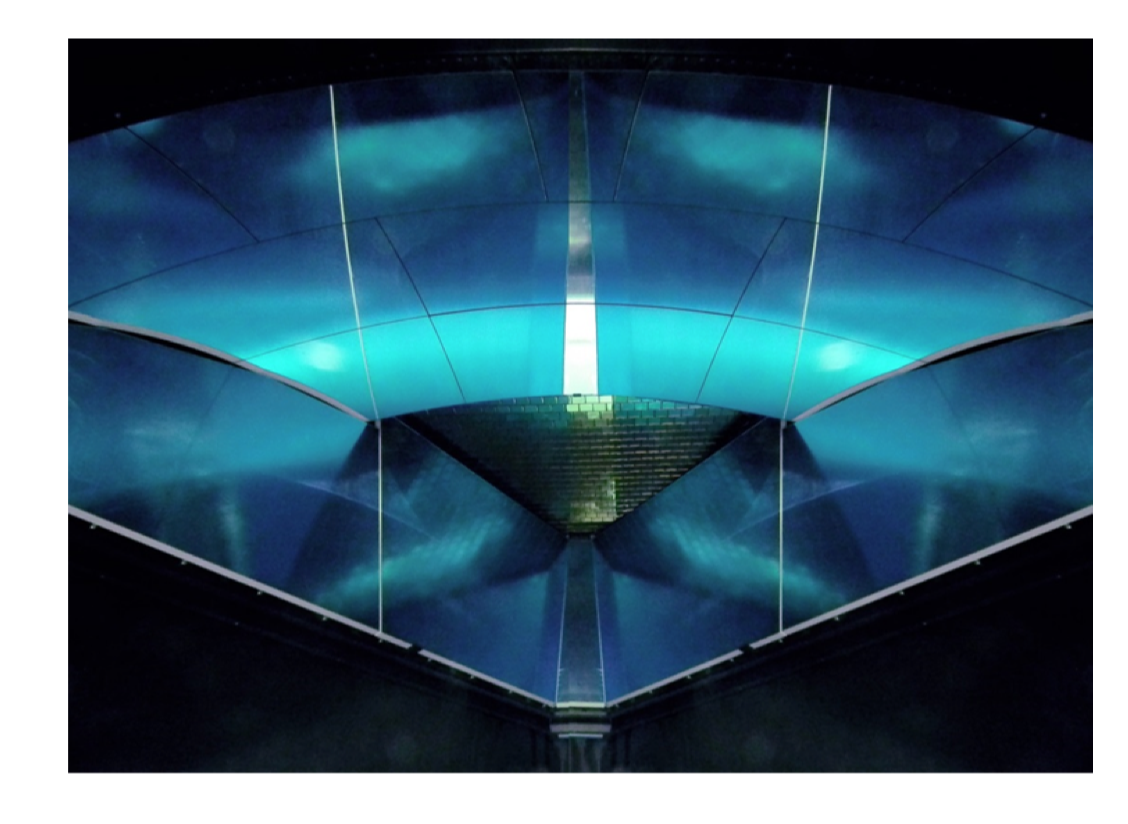
\includegraphics[width=1.0\columnwidth]{rich-mirrors.png}}
\caption{(Color Online) The RICH mirror system shown here in a perspective view as seen from the entrance 
window, with the spherical mirrors above, and
the planar mirrors below. The detector array with the MAPMTs is seen in the center. The aerogel radiator is not shown. }
\label{RICH}
%\end{figure}
%\begin{figure}[htbp!]
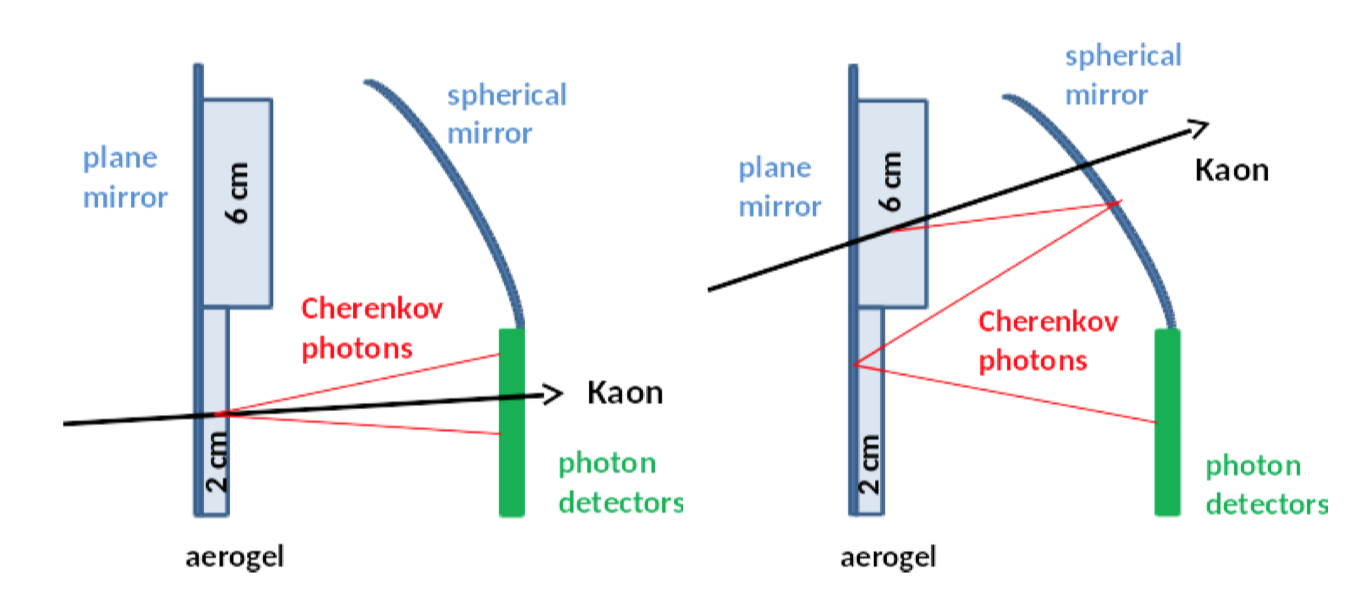
\includegraphics[width=1.0\columnwidth]{rich.png}
\caption{(Color Online) The principle operation and the optics of the
RICH detector. The left panel shows the optics for direct light detection, the right panel shows the optics for reflected photon detection.}
\label{RICH-optics}
\end{figure}

\subsection{Forward Time-of-Flight (FTOF)}
\label{ftof}

The FTOF system is part of the Forward Detector and is used to measure the time-of-flight of charged particles 
emerging from the production target during beam operation. It includes six sectors of plastic scintillators with 
double-sided PMT readout. Each sector consists of three arrays of counters (panel-1a - 23 counters, panel-1b 62
counters, panel-2 5 counters). The system is required for excellent timing resolution for particle identification and
good segmentation for flexible triggering options. The detectors span a range in polar angle from $5^\circ$ to
$35^\circ$, covering 50\% in $\phi$ at $5^\circ$ and 90\% at $35^\circ$. The lengths of the counters ranges from
32.3~cm to 376.1~cm in panel 1a, from 17.3~cm to 407.9~cm in panel-1b, and from 371.3~cm to 426.2~cm in panel-2.
The average timing resolution in panel-1a is 125~ps, 85~ps in panel-1b, and 155~ps in panel-2. Figure~\ref{ftof-1b}
shows the FTOF system on the Forward Carriage. For details of the FTOF construction and performance, see
Ref. ~\cite{FTOF}. 

\begin{figure}[htbp!]
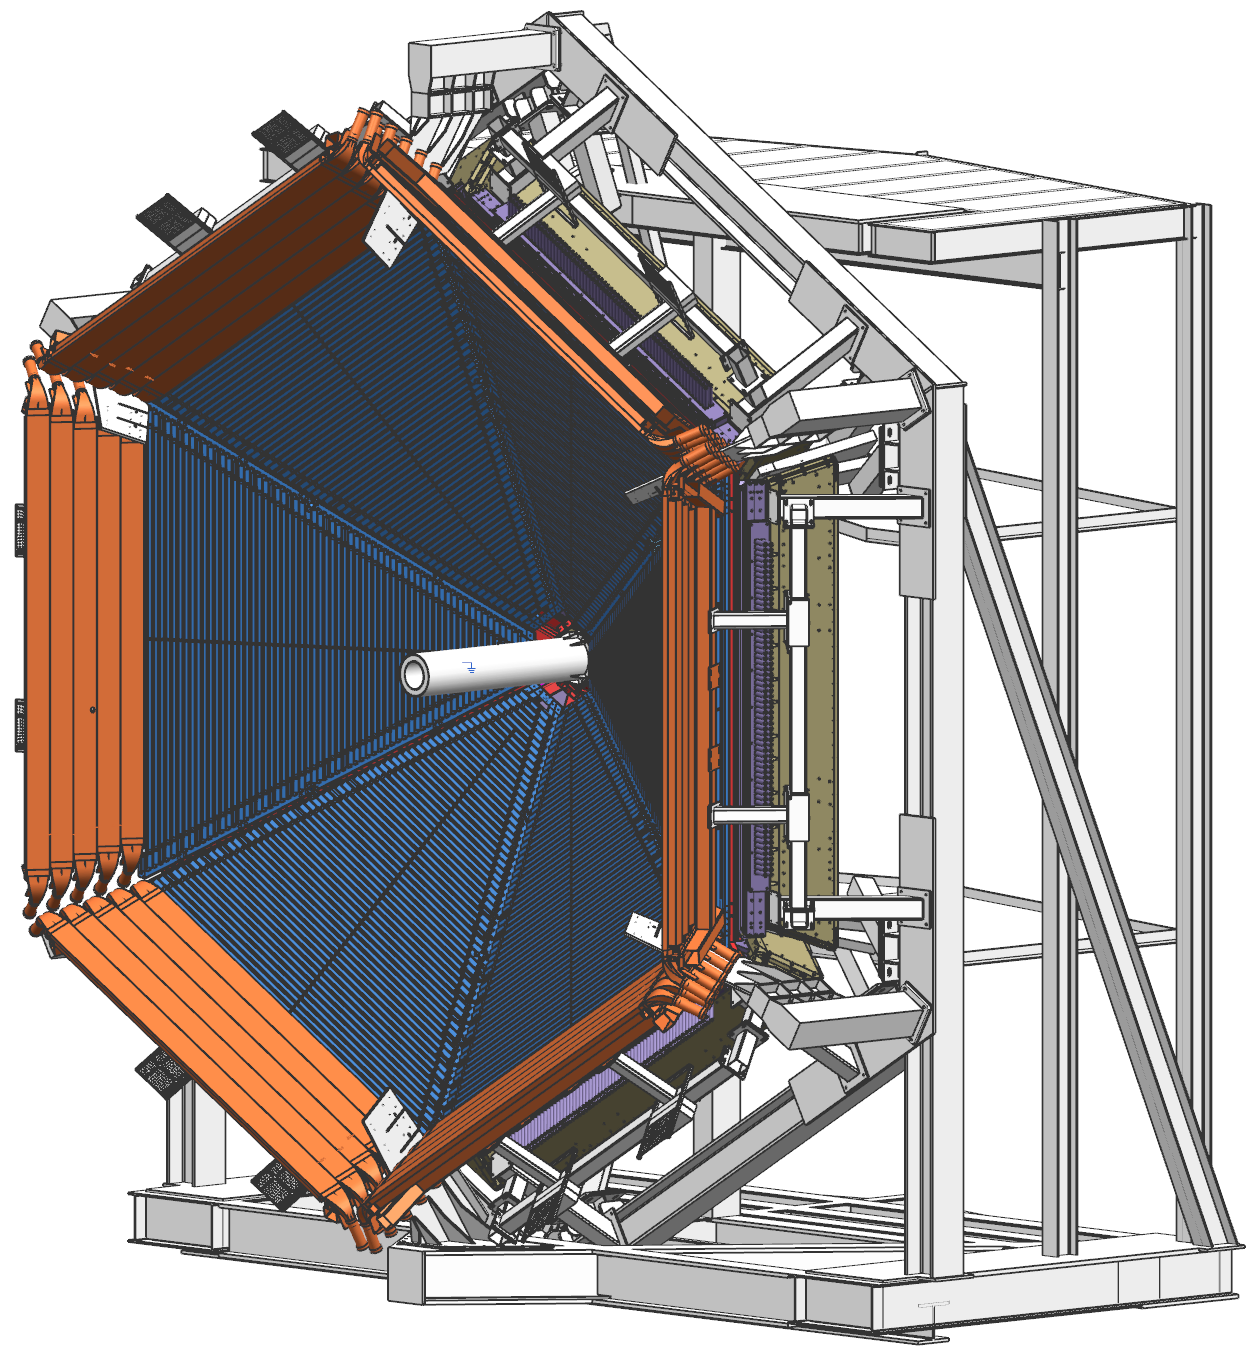
\includegraphics[width=0.95\columnwidth]{fwd_carriage-1.png}
\caption{(Color Online) 3D rendering of the Forward Carriage with the FTOF system showing the panel-1b counters on the
inside, and the panel-2 counters on the outside. The panel-1a counters are located immediately downstream of the
panel-1b counters and are not visible here. Part of the PCAL is visible downstream of the FTOF panels}. 

\vspace{0.5cm} 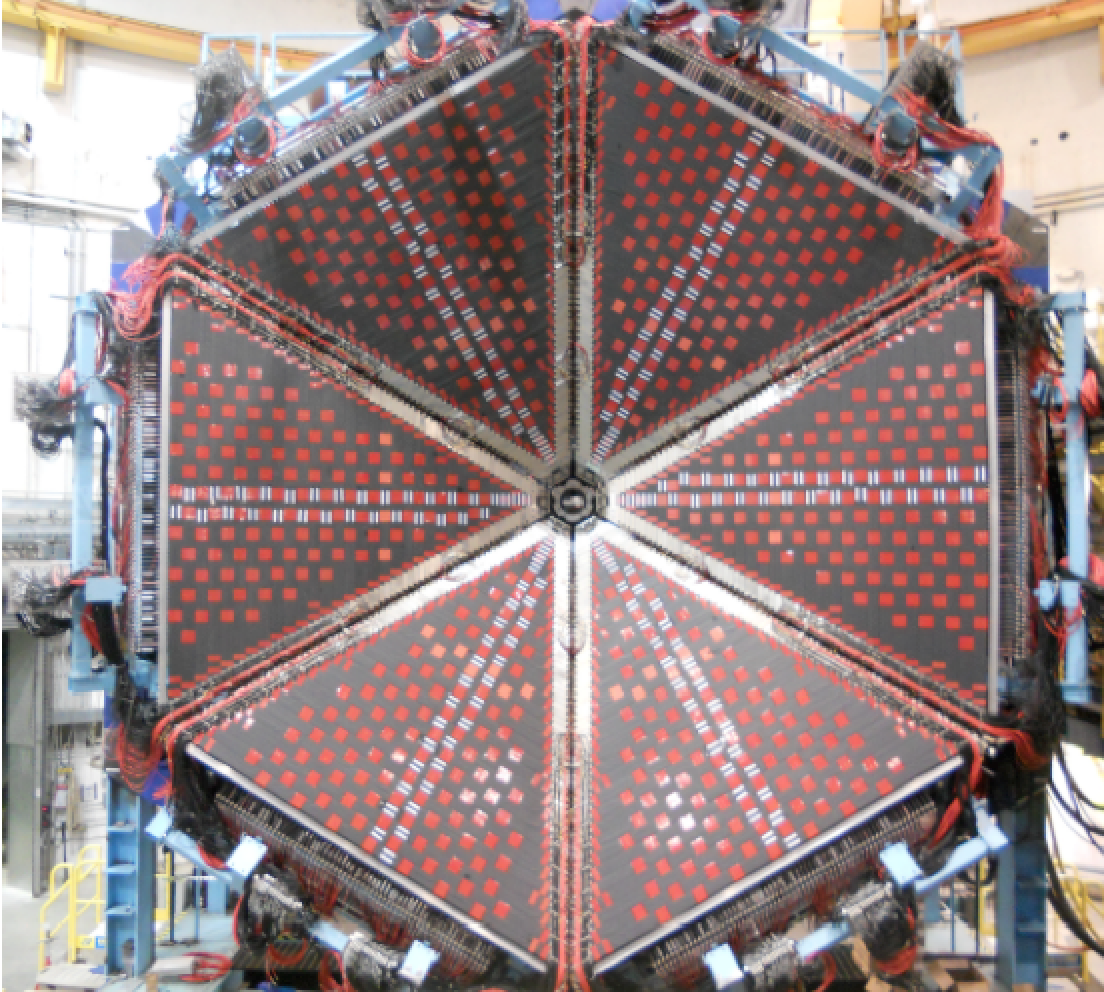
\includegraphics[width=1.0\columnwidth]{FTOF-1b.png}
\caption { (Color Online) Photograph of the FTOF panel-1b counters mounted on the CLAS12 Forward Carriage 
in front of panel-1a and PCAL.} 
\label{ftof-1b}
\end{figure}

\begin{figure}[htbp!]
\centerline{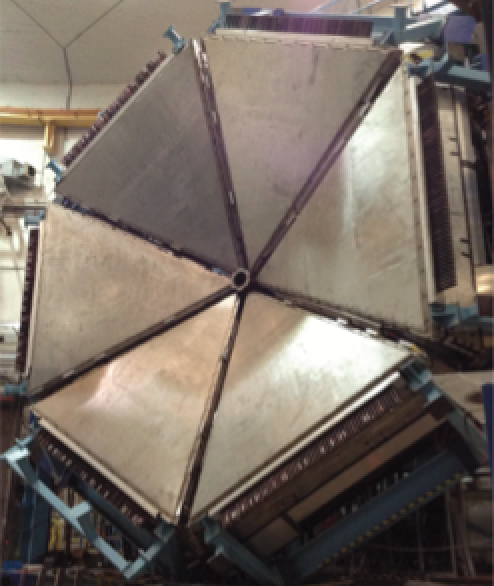
\includegraphics[width=0.95\columnwidth]{PCAL.png}}
\caption{(Color Online) PCAL after installation on the Forward Carriage in front of the existing EC. }
\label{ec-pcal}
\end{figure}
%\vfill

\subsection{Electromagnetic Calorimeters (ECAL)}

The CLAS12 detector package uses the existing electromagnetic calorimeter (EC) of the CLAS detector
\cite{Amarian:2001zs} and a new pre-shower calorimeter (PCAL) installed in front of it. The calorimeters in
CLAS12 are used primarily for the identification and kinematical reconstruction of electrons, photons (e.g. from
$\pi^0 \to \gamma \gamma$ and $\eta \to \gamma  \gamma$ decays ), as well as the detection of neutrons.
For details of the construction and the performance of the PCAL calorimeter (see Ref.~\cite{ECAL}). 

The PCAL and EC are both sampling calorimeters consisting of six modules. The EC consists of EC-inner and
EC-outer parts, which are separately read out. Each module has a triangular shape with 54 (15/15/24,
PCAL/EC-inner/EC-outer) layers of 1-cm thick scintillators segmented into 4.5/10-cm (PCAL/EC) wide strips
sandwiched between 2.2~mm thick lead sheets. The total thickness corresponds to approximately 20.5 radiation
lengths. Scintillator layers are grouped into three readout views with 5/5/8, PCAL/EC-inner/EC-outer, layers per
view, providing several cm resolution of energy clusters. The light from each scintillator readout group is routed to
the photomultiplier tubes via flexible optical fibers. Figure~\ref{ec-pcal} shows the PCAL after installation on the
Forward Carriage in front of the existing EC from CLAS.

\begin{figure}[t!]
\centerline{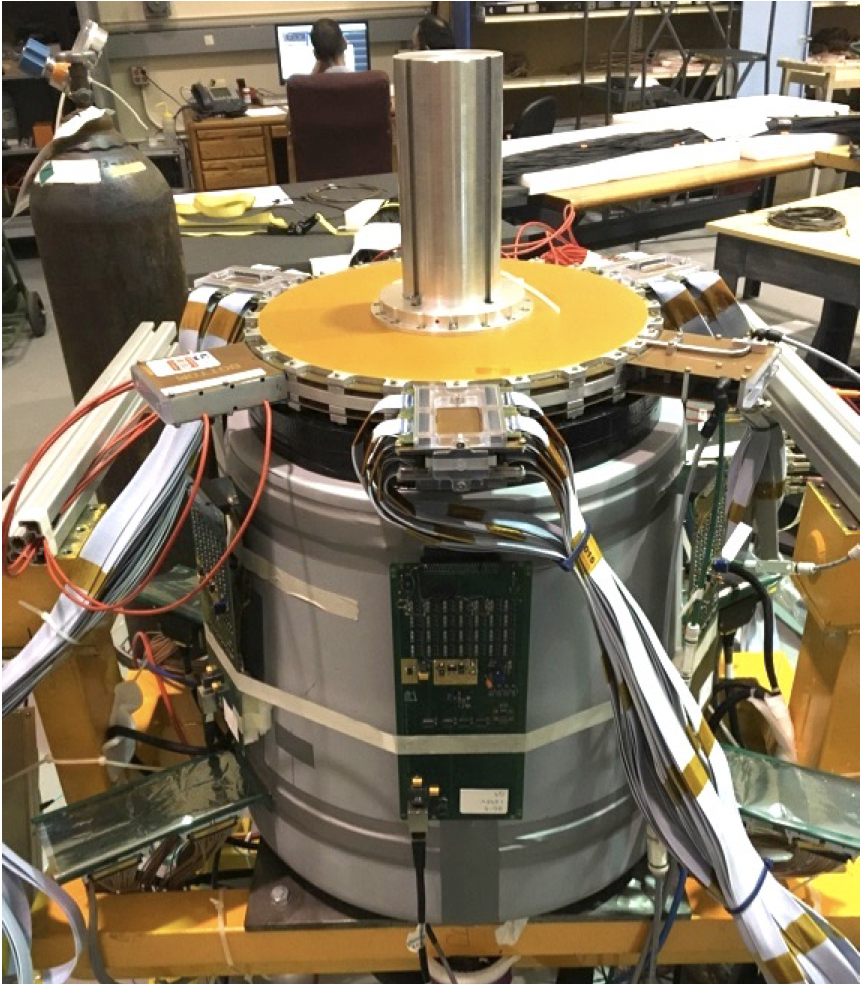
\includegraphics[width=0.75\columnwidth]{FT-photo.png}}
\caption{(Color Online) The Forward Tagger system during cosmic ray testing before installation in CLAS12. The lower part contains
the electromagnetic calorimeter composed of lead-tungstate crystals. The upper part includes the hodoscope and the
tracking disks.}
\label{ft-photo}
%\end{figure}
%\begin{figure}[htbp!]
\vspace{1cm}\centerline{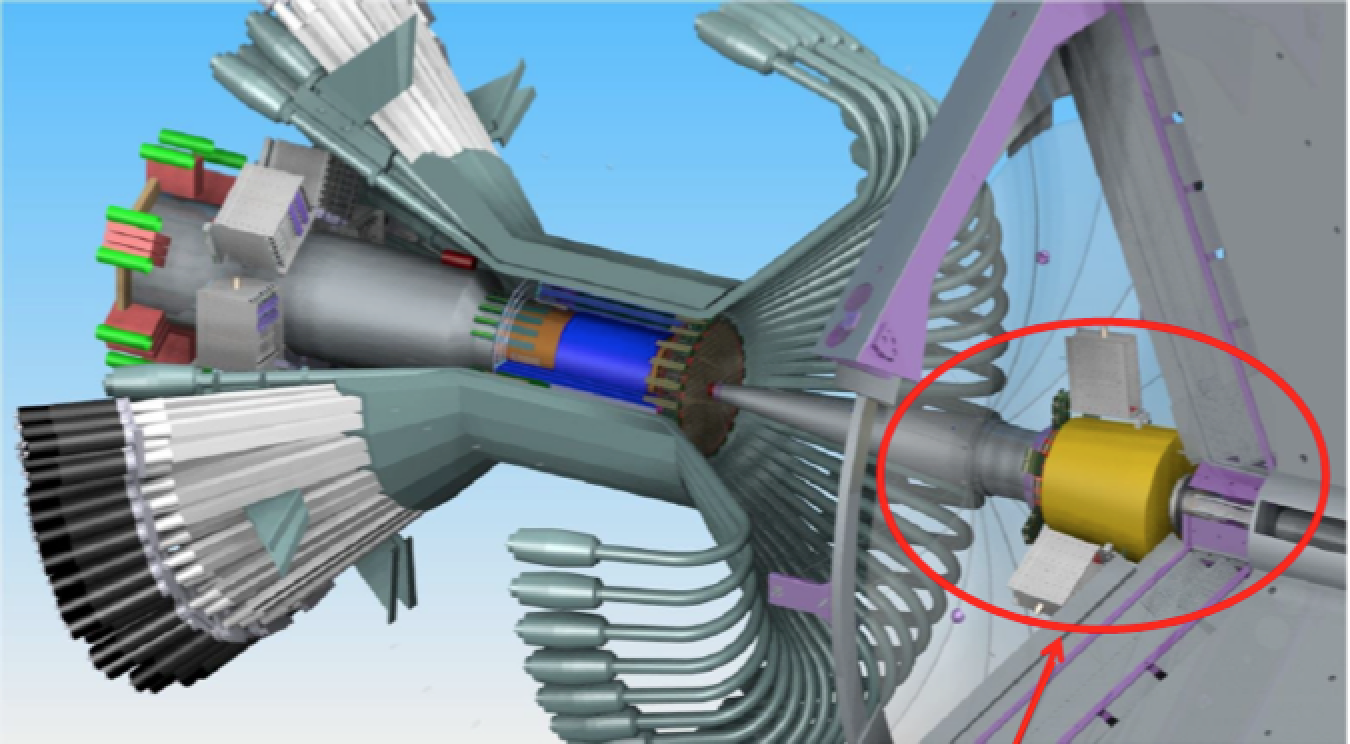
\includegraphics[width=1.0\columnwidth]{CD-FT.png}}
\caption{(Color Online) The Forward Tagger system (circled) downstream of Central Detector in front of the Torus magnet warm
bore entrance.}
\label{ft}
\end{figure}

\section{CLAS12 Central Detector (CD)} 
\begin{figure}[t!]
\centerline{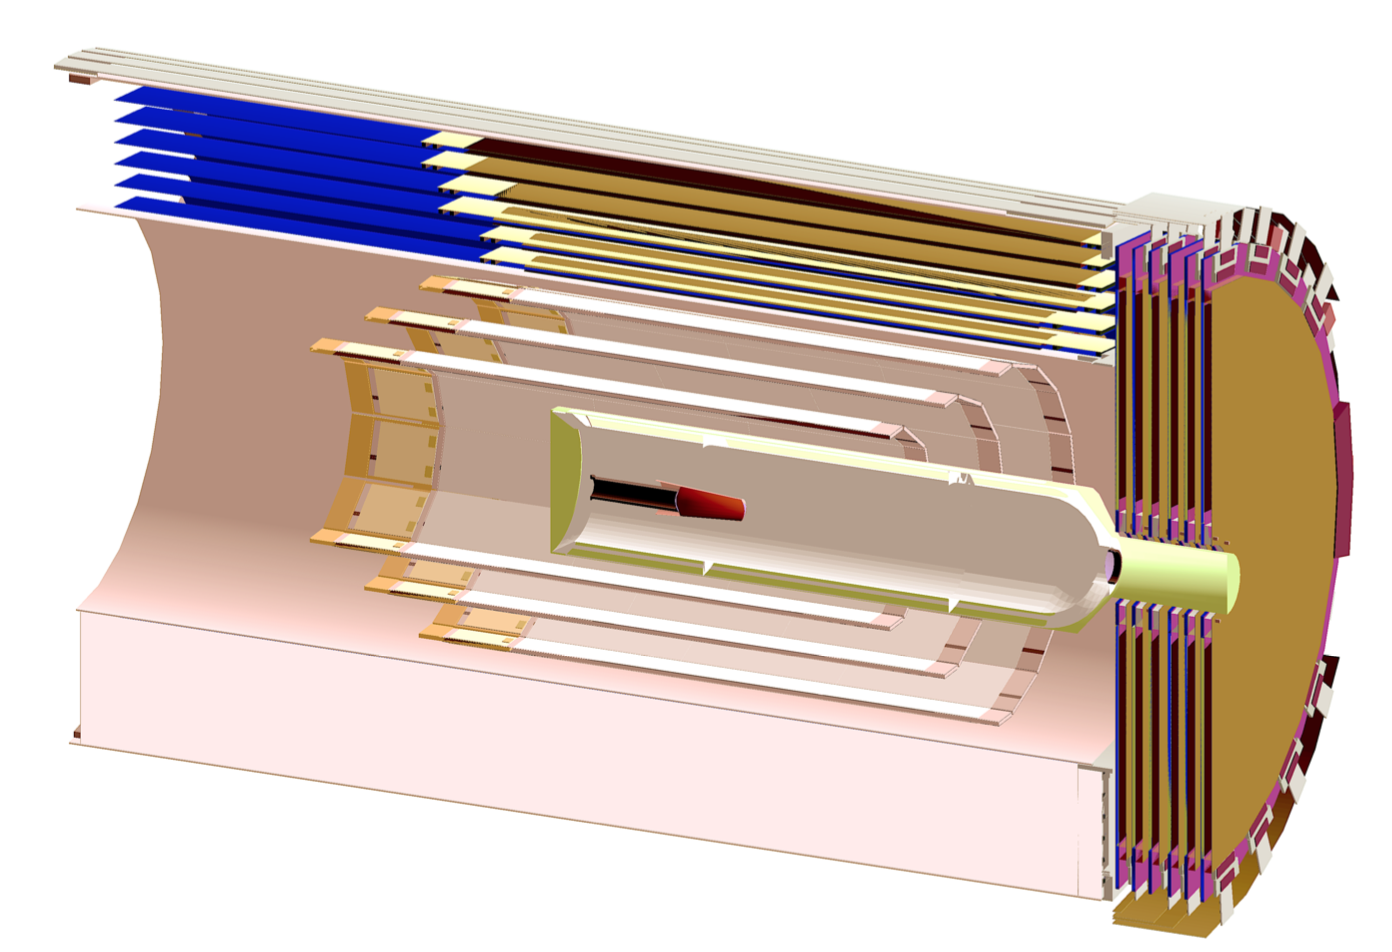
\includegraphics[width=1.0\columnwidth]{CVT-schematics.png}}
\caption{ \rm Central Vertex Tracker schematics, showing (from the inside) the target cell and vacuum chambers, the 3 double layers of the SVT, followed by the 6 layers of BMT. The beam enters from the left.  The six FMT layers are shown at the downstream end at the 
right. }
\label{CVT}
%\end{figure}
\vspace{1.0cm}
%\begin{figure}[htbp!]
\centerline{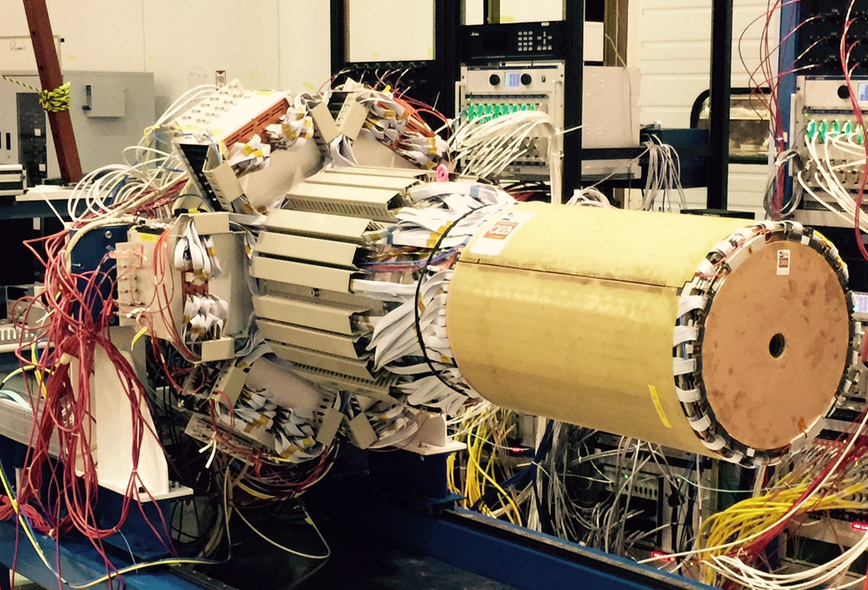
\includegraphics[width=1.0\columnwidth]{CVT.png}}
\caption{(Color Online) Central Vertex Tracker, fully assembled with the SVT, BMT, and FMT. The BMT and FMT are shown on the
outside. The SVT is encapsulated and hidden from view.}
\label{CVT}
\end{figure}
\subsection{Forward Tagger (FT)}
\begin{figure}[htbp!]
\centerline{\includegraphics[width=1.0\columnwidth]{solenoid-photo.png}}
\caption{(Color Online) The Central Detector installed in the Solenoid magnet in a side view. The readout photomultiplier tubes are
seen at the upstream end (left) and at the downstream end (right) of the Solenoid.}
\label{CDinSol}
\end{figure}


\begin{figure}[htbp!]
\centerline{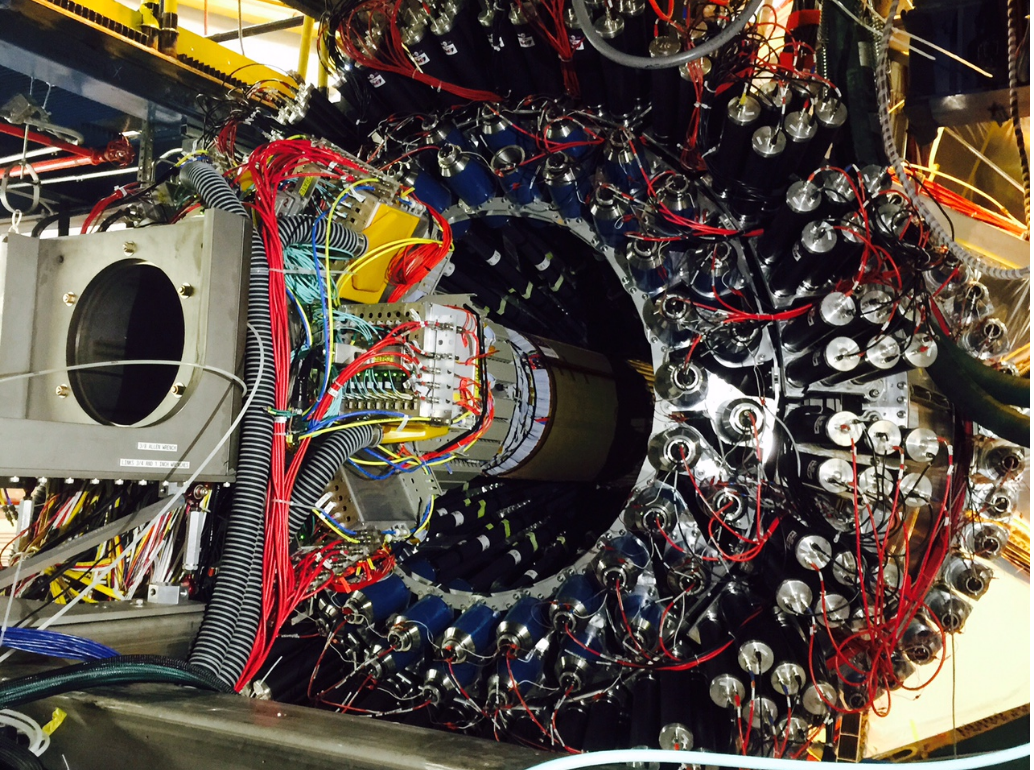
\includegraphics[width=1.3\columnwidth,angle=90]{CLAS12-CD.png}}
\caption{(Color Online) The Central Detector seen from the upstream end. The CVT is shown in a retracted position for
maintenance. During operation the CVT is fully inserted into the warm bore of the magnet.}
\label{CDback}
\end{figure}
Particles scattered at polar angles from $2.5^\circ \le \theta \le 4.5^\circ $ are detected in the calorimeter, the
micro-strip gas tracker, and the hodoscope of the Forward Tagger (FT). The FT extends the CLAS12 capabilities to
detect electrons and photons at very forward polar angles. The detection of forward-going scattered electrons allows
for electroproduction experiments at very low photon virtuality $Q^2$, providing an energy-tagged, linearly polarized,
high-intensity, quasi-real photon beam. This configuration enables execution of an extensive hadron spectroscopy
program. The FT is comprised of an electromagnetic calorimeter with 332 lead-tungstate (PbWO$_4$) crystals to
identify electrons,  measure the electromagnetic shower energy, and provide a fast trigger signal. The tracking system
in front of the calorimeter  measures the scattering angles, and a scintillator hodoscope aids in separating electrons and
high-energy photons. Figure~\ref{ft-photo} shows a photograph of the FT during cosmic ray studies before its installation
in CLAS12. 
During beam operation the FT can be used in two configurations that serve requirements of different experiments. In the FT-OFF 
configuration the FT is in-active and all electronics channels are turned off. This allows use of the FT calorimeter supplemented by 
an additional lead shield, as an effective shielding element of the DC R1 against low energy background. This reduces the 
accidental background by 1/3 at the same beam conditions. Further details on the FT are described in Ref.~\cite{FT}. Figure~\ref{ft} shows a rendering of the FT setup near the entrance to the warm bore of the Torus magnet.   



Particles scattered from the target at polar angles in the range from $35^\circ$  to $120^\circ$ are detected in the
Central Detector with its own particle identification and tracking detectors. Charged particles are detected in the
Central Time-of-Flight (CTOF) detector with full $360^\circ$ coverage in azimuthal angle, and tracked in the Central
Vertex Tracker (CVT). Neutron detection is provided by the Central Neutron Detector (CND) located radially outside
of the CVT and the CTOF.  Figure~\ref{CVT} shows the fully assembled CVT before installation in the solenoid magnet.
The fully assembled CD is displayed in  Figure~\ref{CDinSol} after installation in the Solenoid.  Figure~\ref{CDback}
shows the installed Central Detector from the upstream end.



\begin{figure}[t!]
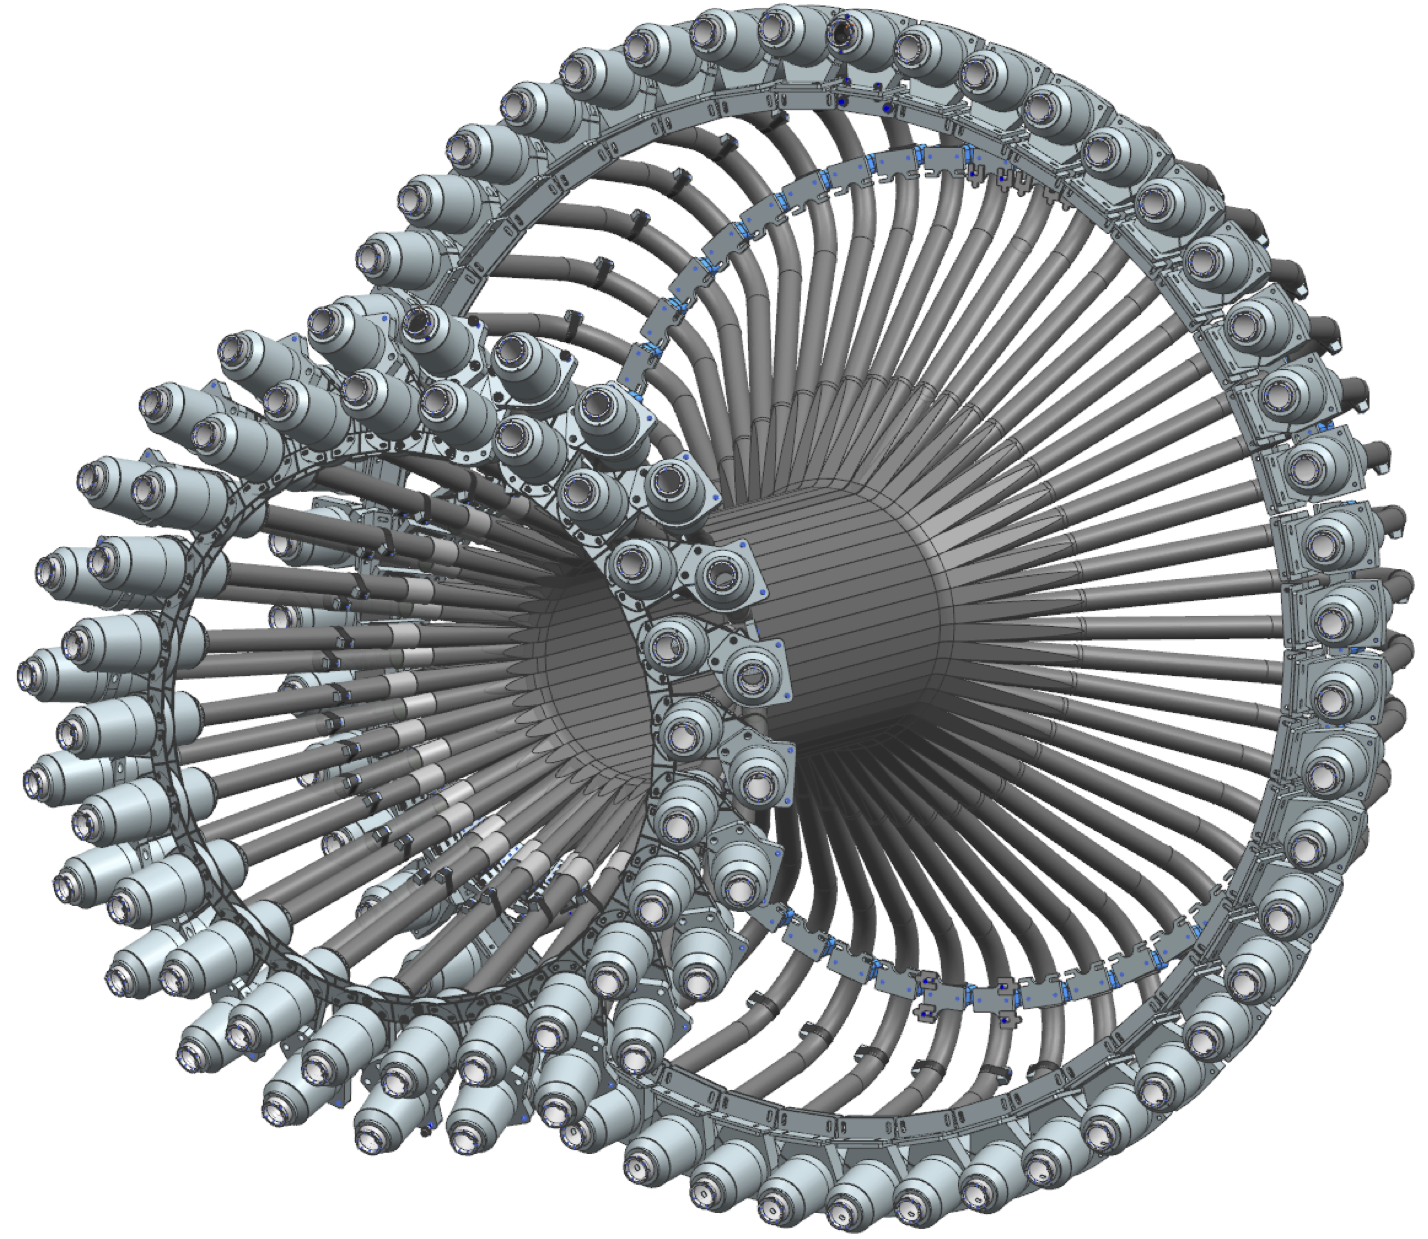
\includegraphics[width=1.0\columnwidth]{ctof-design.png}
\caption{(Color Online) The Central Time-of-Flight detector with the 48 scintillator bars, and the 48 photomultipliers on each end
of the scintillators.} 
\vspace{0.5cm}\centerline{\includegraphics[angle=90,width=0.9\columnwidth]{cnd-ctof.png}}
\caption{(Color Online) The fully assembled CD as seen from its upstream end with the 144 CND light guides and
photomultipliers at the three outermost rings, and the 48 PMTs of the CTOF (two inner rings). } 
\label{ctof-cnd}
\end{figure} 


\subsection{Central Vertex Tracker (CVT)}

The CLAS12 CVT is a part of the Central Detector and is used to measure the momentum and determine the vertex of
charged particles scattered from the production target, which is centered within the Solenoid magnet. It contains two
separate trackers, a Silicon Vertex Tracker (SVT) and a Barrel Micromesh Tracker  (BMT). The SVT system includes
3 regions with 10, 14, and 18 sectors of double-sided modules of silicon sensors instrumented with digital readout ASICs
and FSSR2s. The readout pitch is 156~$\mu$m, and the total number of channels is 33,792. See Ref.~\cite{SVT} for
details on the design, construction, and performance of the SVT.

The BMT contains 3 layers of strips along the beamline and 3 layers of circular readout strips around the beamline, with
a total number of 15,000 readout elements. The BMT provides important improvements in momentum resolution, and in
tracking efficiency. Each layer is arranged azimuthally in 3 sectors of 125$^\circ$ azimuthal coverage. The system
operates at full design luminosity of $10^{35}$~cm$^{-2}$s$^{-1}$. Another component is the Forward Micromegas Tracker
(FMT), consisting of 6 layers with 6,000 readout elements. It  is integrated mechanically with the CVT to provide a compact
tracking system, but covers the polar angle range from 5$^\circ$ to 35$^\circ$ and provides improved vertex reconstruction
for forward scattered charged particles. See Ref.~\cite{BMT} for details on the BMT and on the FMT. \footnote{The FMT tracker has not been implemented during the experimental runs covered in this paper.}  



\subsection{Central Time-of-Flight (CTOF)}

The CTOF system is used for the identification of charged particle emerging from the target via time-of-flight
measurements. The CTOF includes 48 plastic scintillators with double-sided photomultiplier readout via, respectively,
1.0~m-long upstream and 1.6~m-long downstream focusing light guides. The array of counters forms a hermetic barrel
around the target and the CVT. The barrel is aligned with the beam axis inside the 5~T Solenoid magnet. The 
photomultipliers are placed in a region of 0.1~T fringe field of the Solenoid and enclosed within a triple layer dynamical
magnetic shield~\cite{Baturin:2012zz} that provides less than 0.2~G internal field near the PMT photocathode. The
CTOF system is designed to provide time resolution of 80~ps for charged particle identification in the CLAS12 Central
Detector. Details are described in Ref.~\cite{CTOF}. Fig.~\ref{ctof-cnd}(left) shows the CTOF system from the design
model and Fig.~\ref{ctof-cnd}(right) shows the upstream end of the CTOF installed in the Solenoid.

\subsection{Central Neutron Detector (CND)}

The CLAS12 CD is also equipped with the CND that follows the CTOF radially and allows the detection of neutrons in
the momentum range from 0.2~GeV to 1.0~GeV by measurement of their time-of-flight from the target to the hit
position and the energy deposition in the scintillator layers. The detector is made of three layers of scintillator
paddles (48 paddles per layer), coupled two-by-two at the downstream end with semi-circular light guides and read out
at the upstream end by photomultipliers placed outside of the high magnetic field region. The scintillators are connected
to 1.5-m-long bent light guides. The CND is the last radial detector within the warm bore of the Solenoid magnet cryostat. 
Figure~\ref{ctof-cnd} (right) shows the upstream readout end of the CND installed in the Solenoid. Details are described
in Ref.~\cite{CTOF}.

\section{CLAS12 Offline Software}  

The CLAS12 offline software system is designed to analyze large amounts of beam-induced experimental data
acquired during production and cosmic ray runs for alignment and calibration purposes. The system is based on a
service-oriented software architecture that consists of three major components, the event reconstruction,
visualization, and calibration monitoring services, as well as detector and event simulations. 

During the CLAS12 design phase a realistic simulation package based on Geant4 was developed to aid in the optimization 
of the detector hardware response to beam interactions in terms of resolution, robustness of operation at high
luminosities, details of the beamline design, and other aspects. 

\subsection{Event Reconstruction} 

Event reconstruction in the CLAS12 FD consists of the identification of charged and neutral particles along with the 
computation of their 3-momenta. Charged-particle reconstruction requires both particle tracking and particle 
time-of-flight (TOF) information. 
\begin{figure*}[htbp!]
\centerline{
	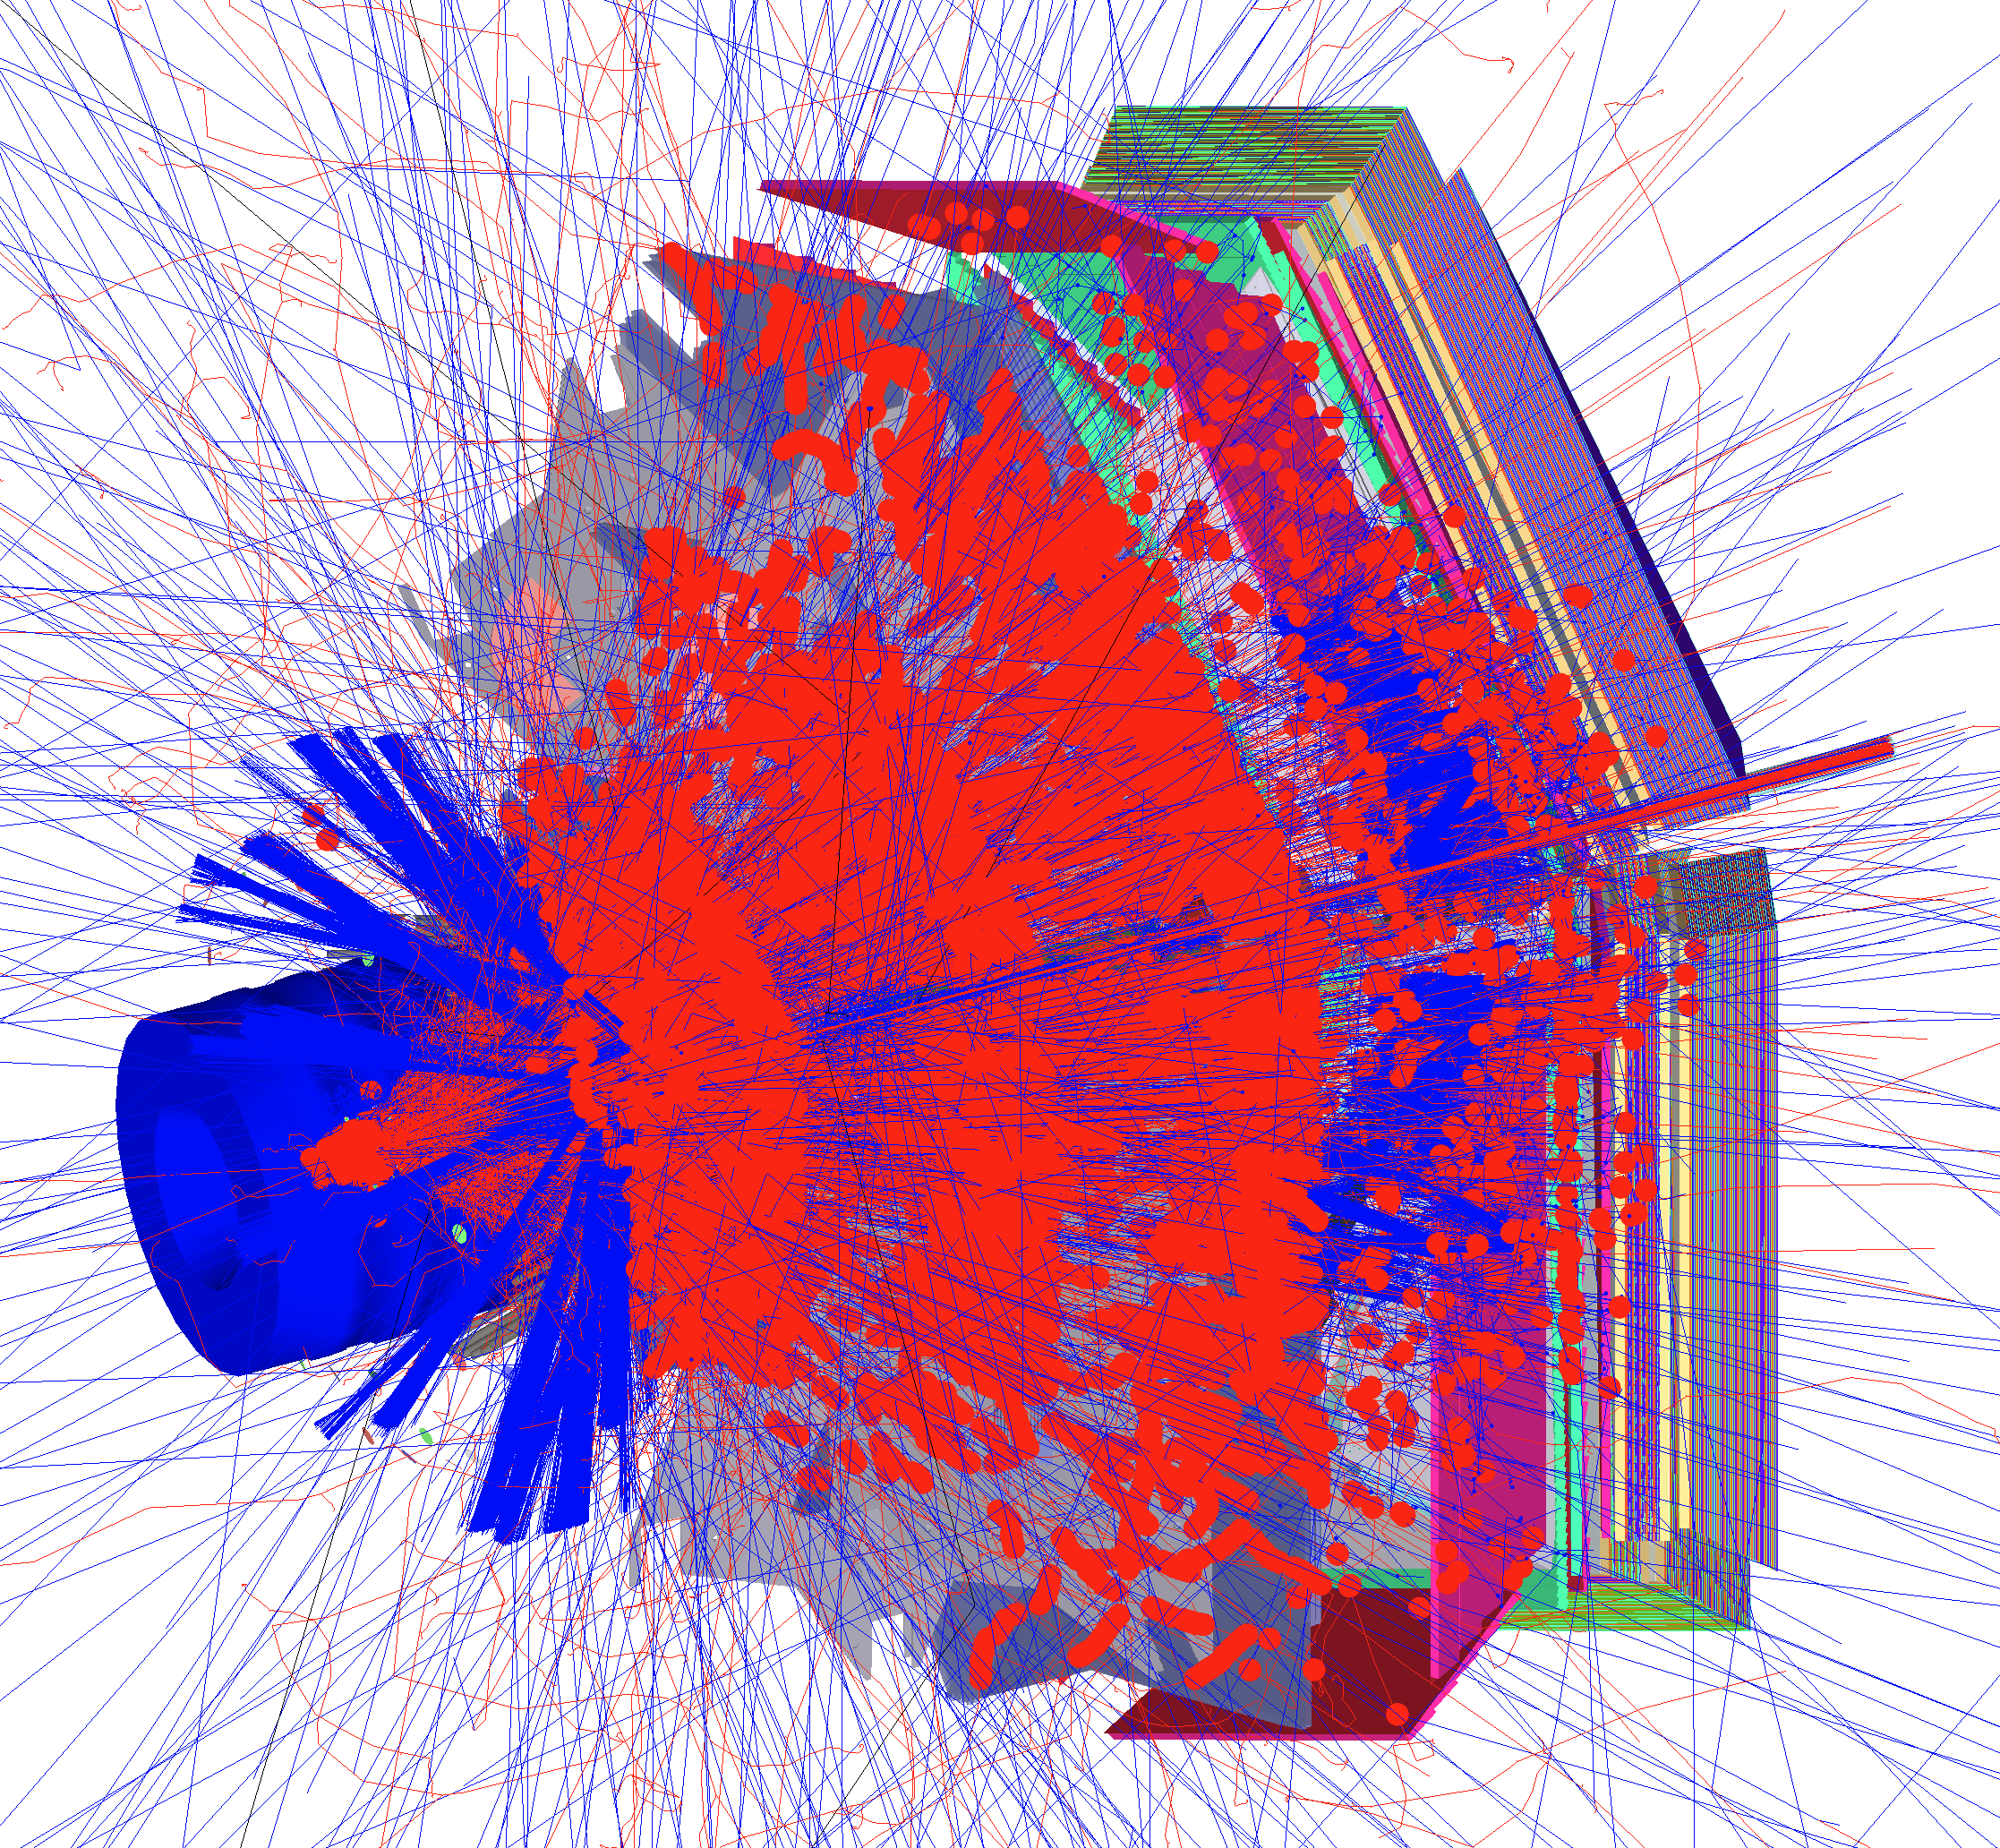
\includegraphics[width=1.0\columnwidth, height=1.0\columnwidth]{NoField.png}
	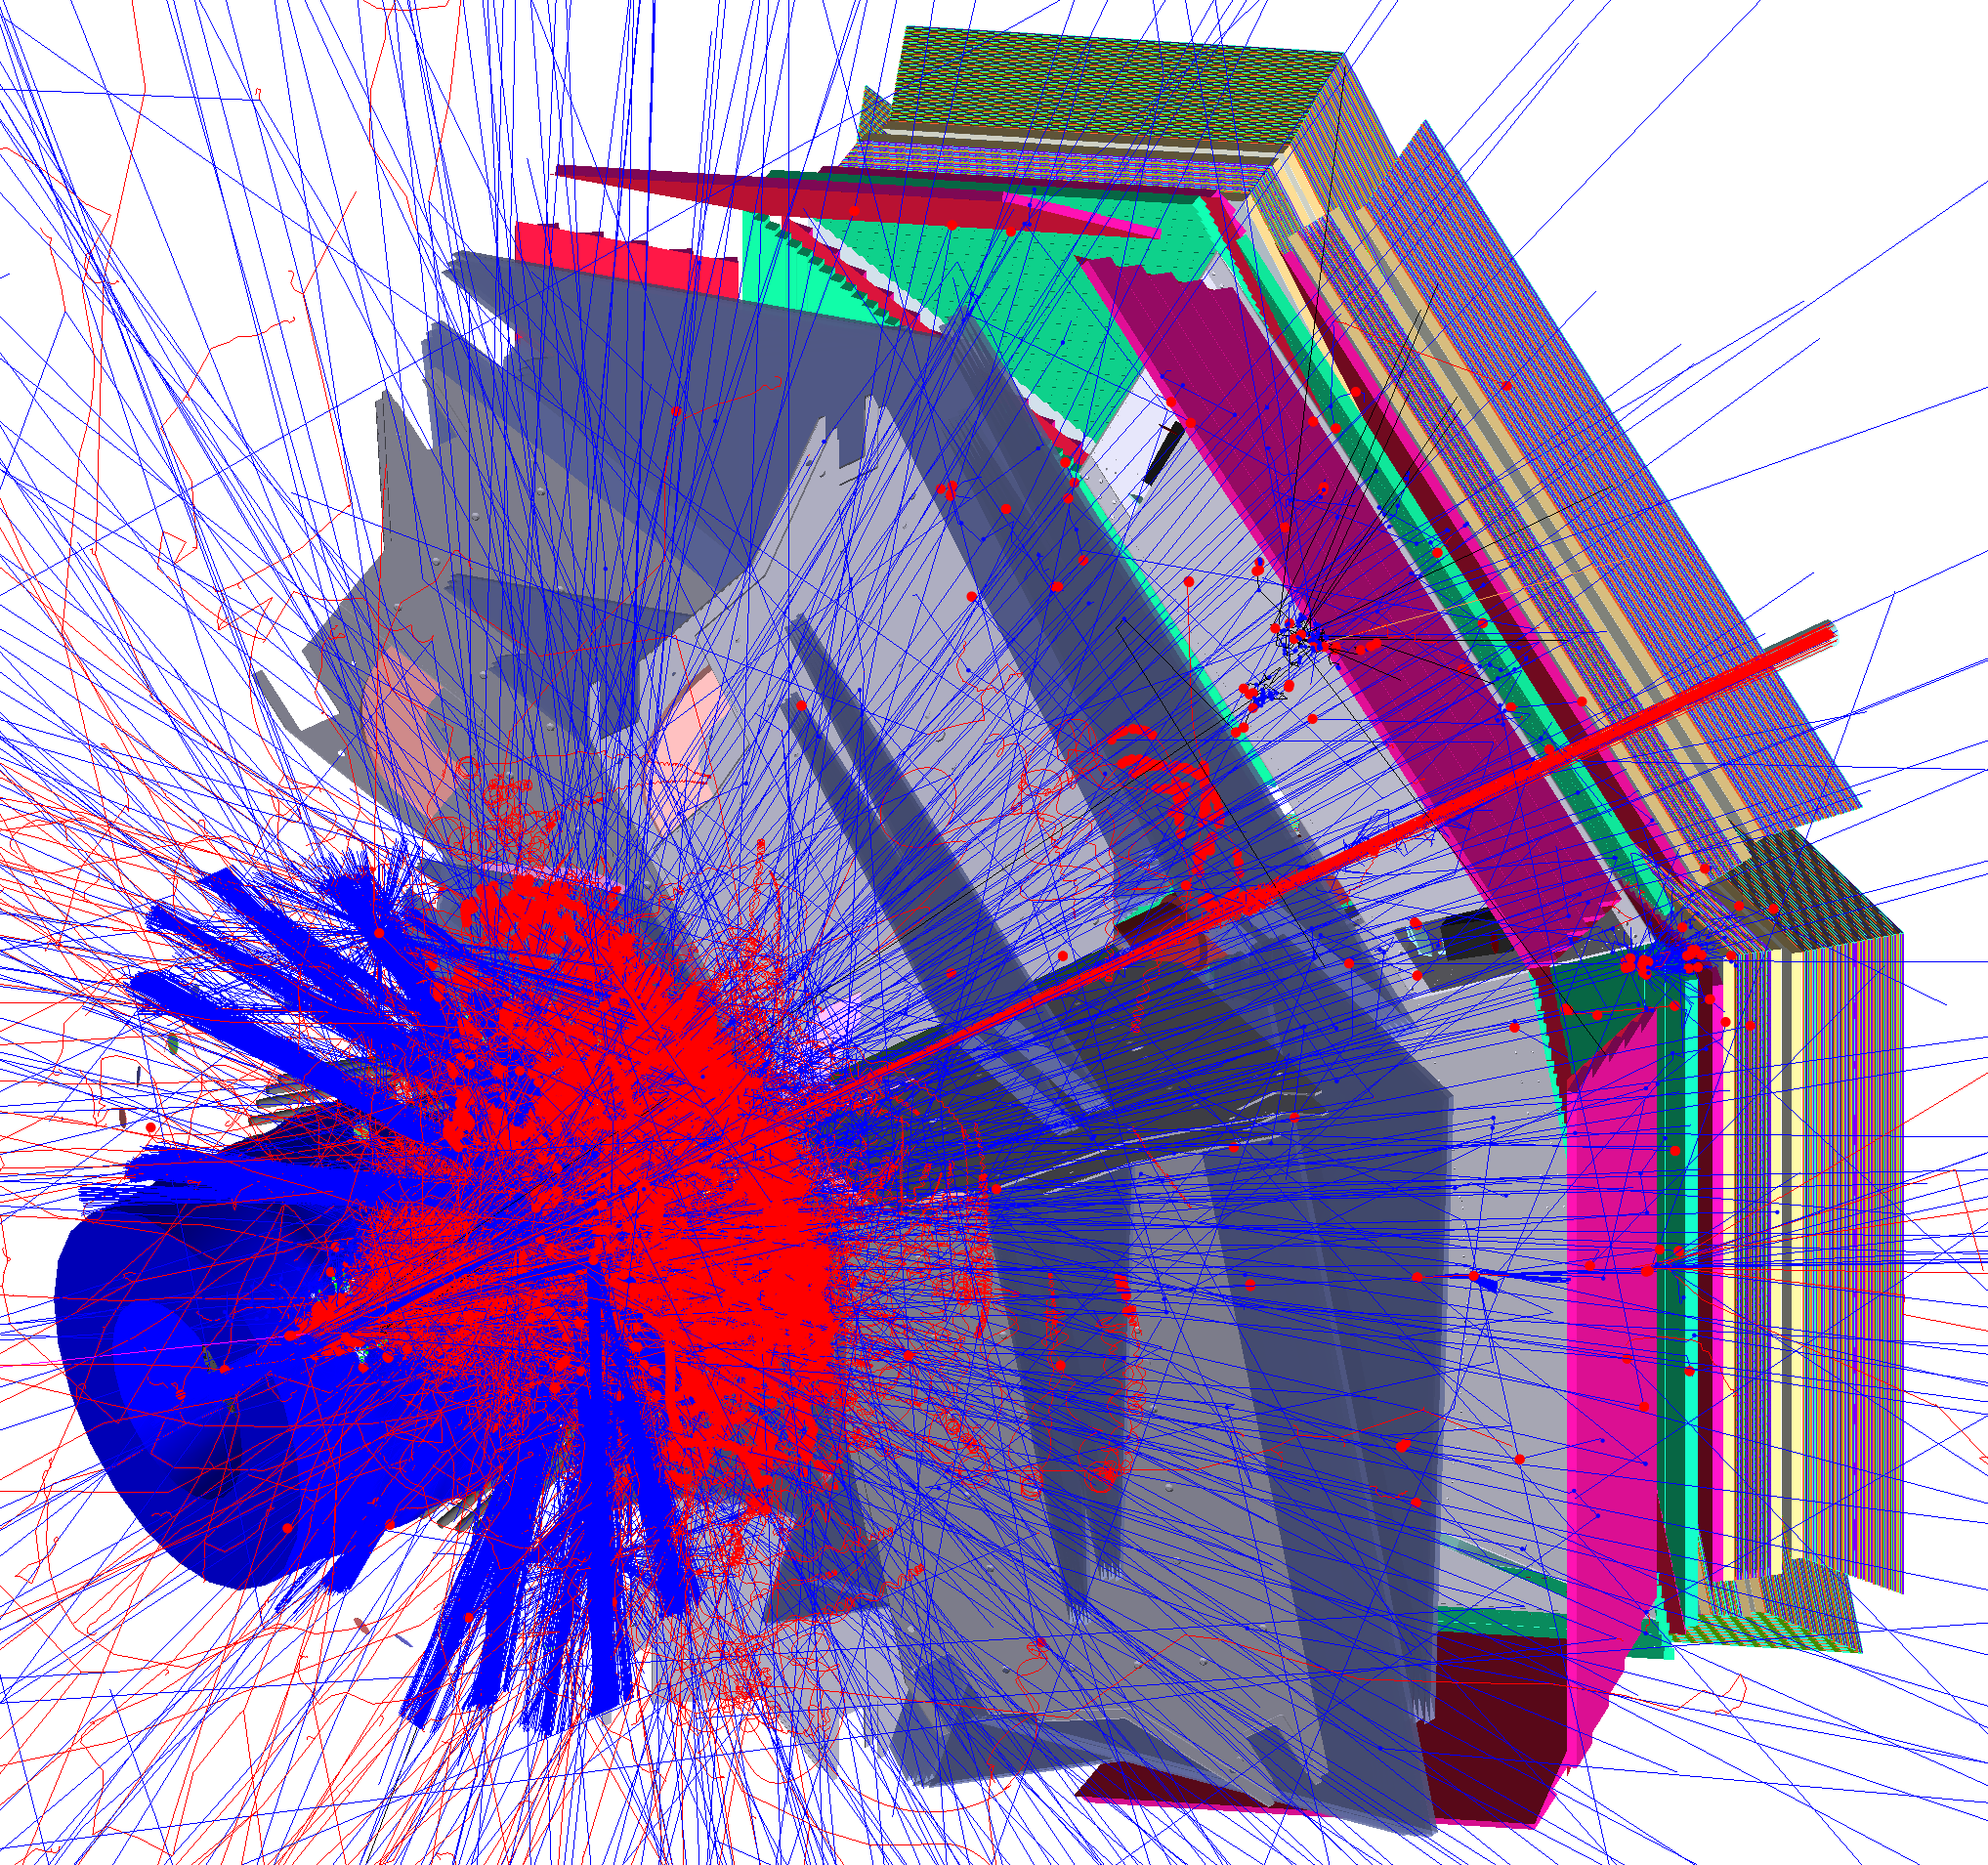
\includegraphics[width=1.0\columnwidth, height=1.0\columnwidth]{NoSolenoidFullTorus.png}
}
\vspace{0.3cm}
\centerline{
	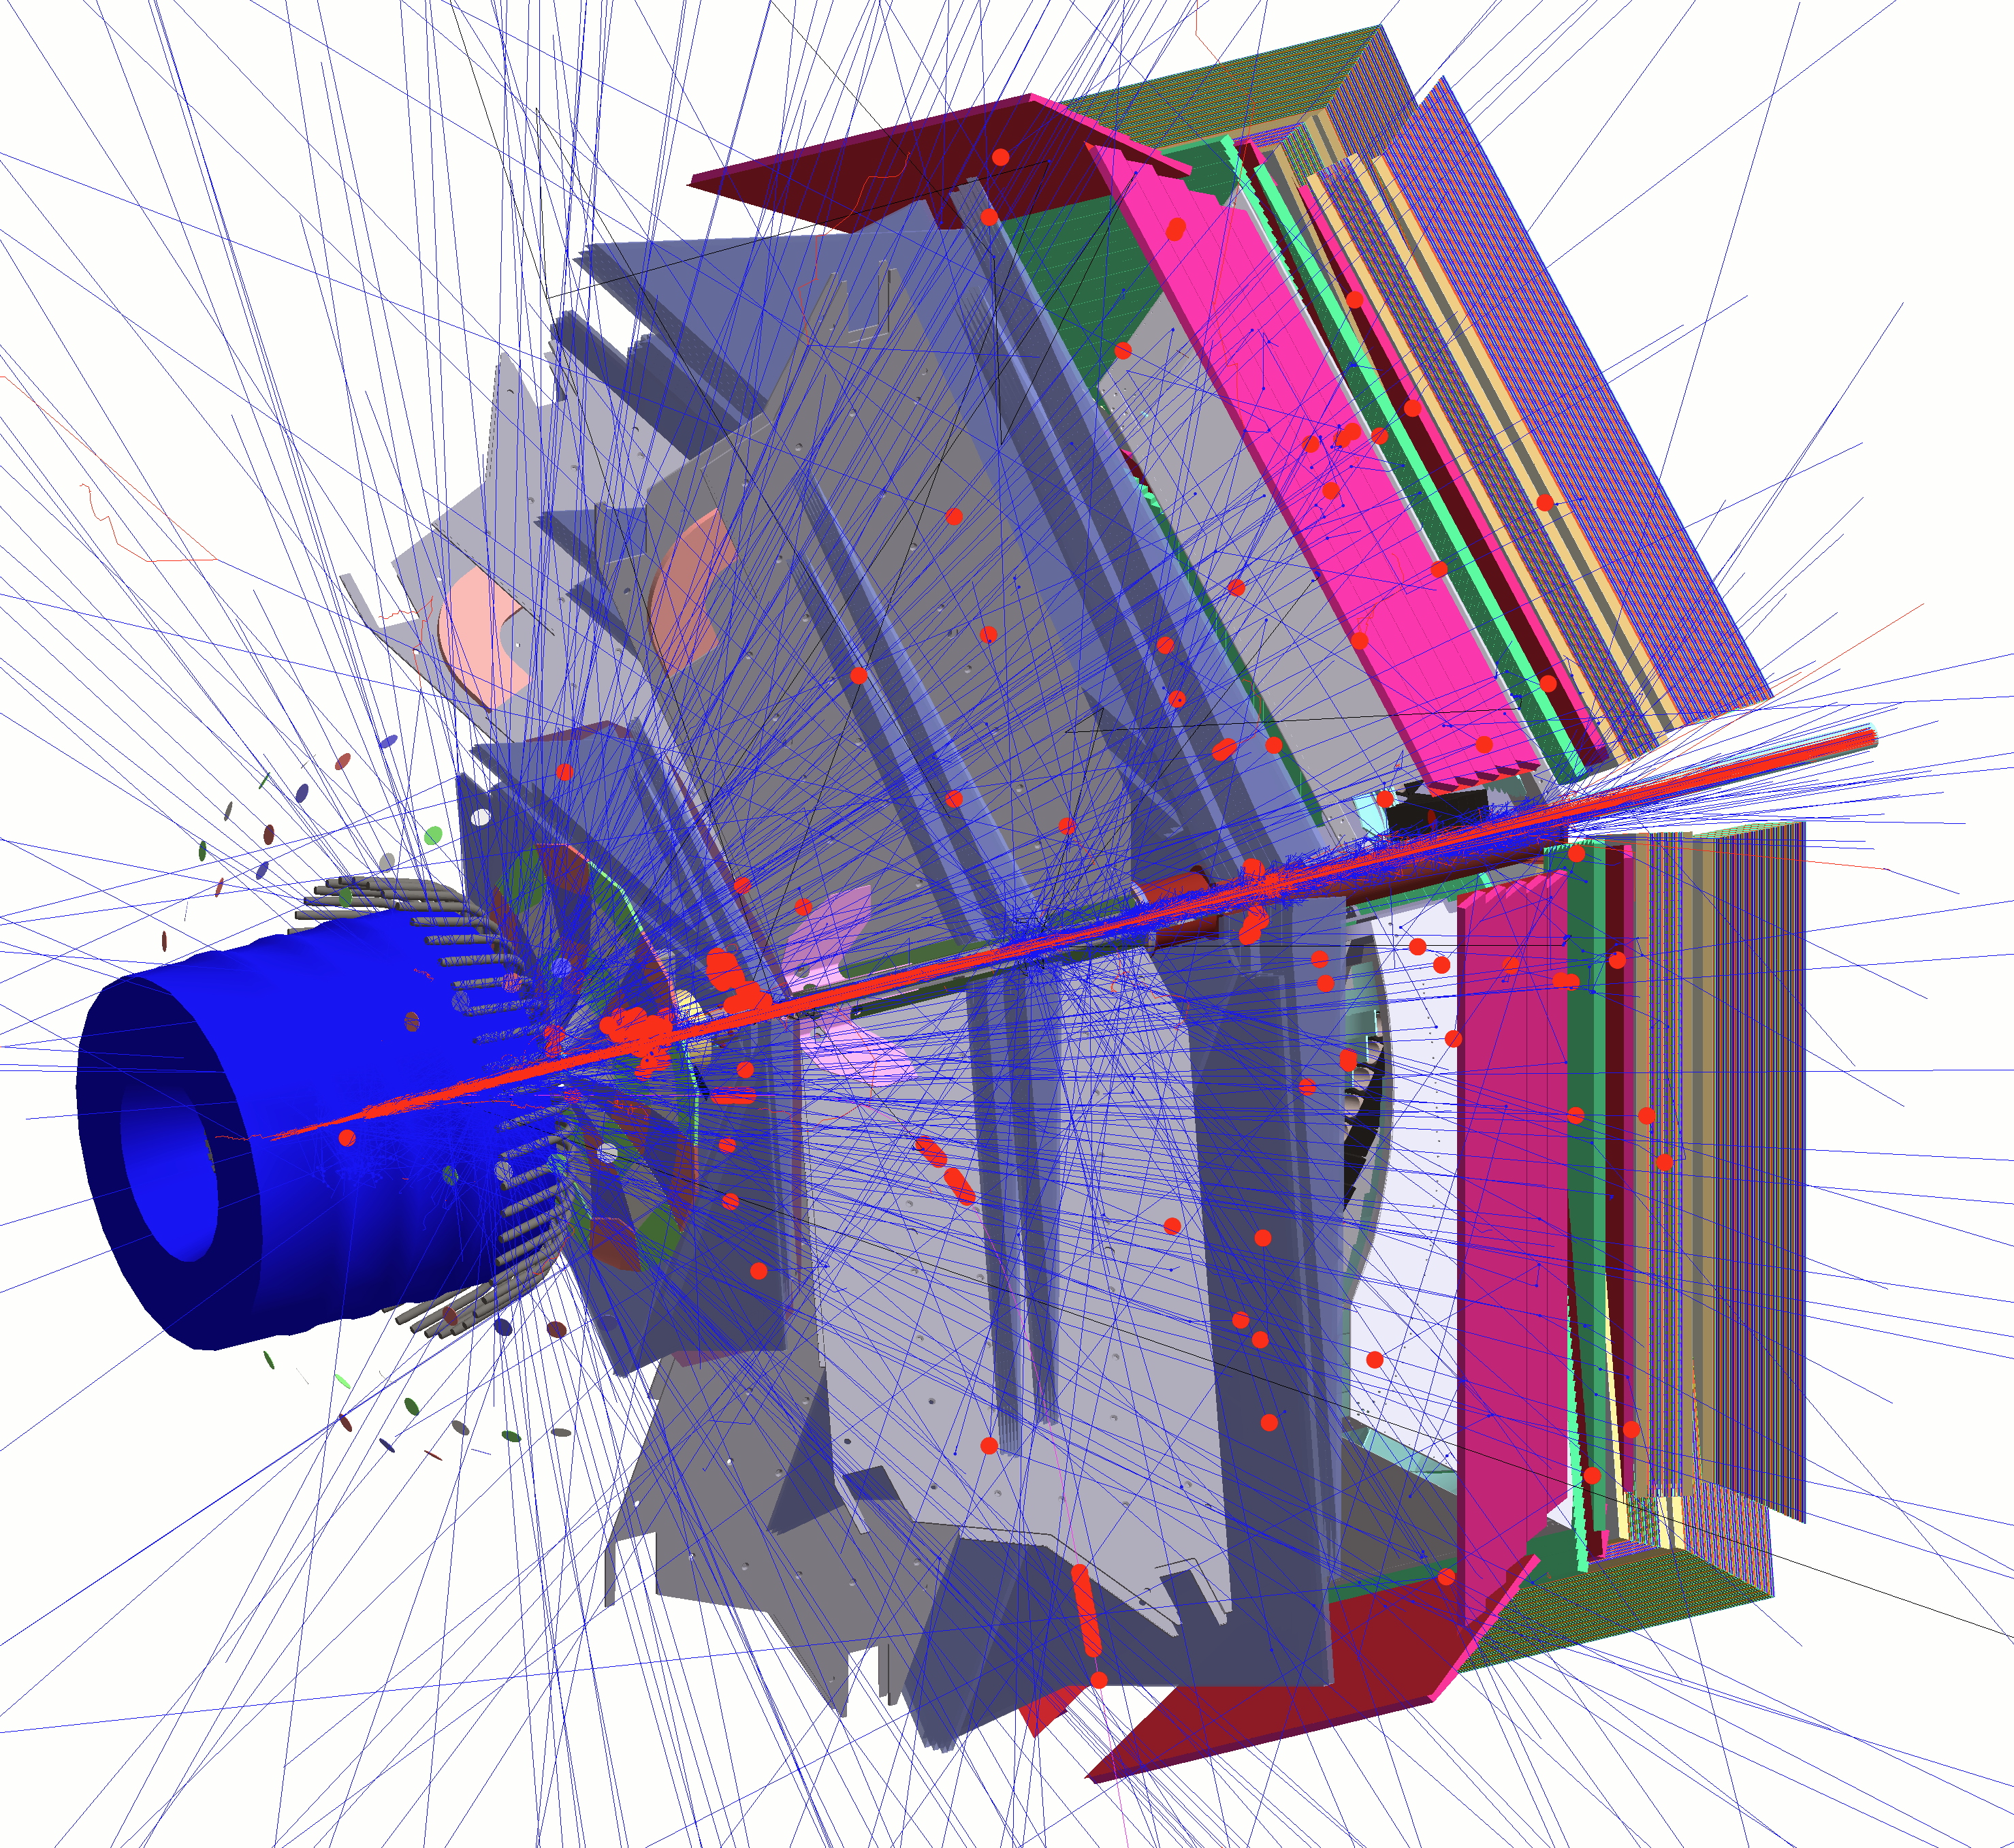
\includegraphics[width=1.0\columnwidth, height=1.0\columnwidth]{FullSolenoidFullTorus.png}
	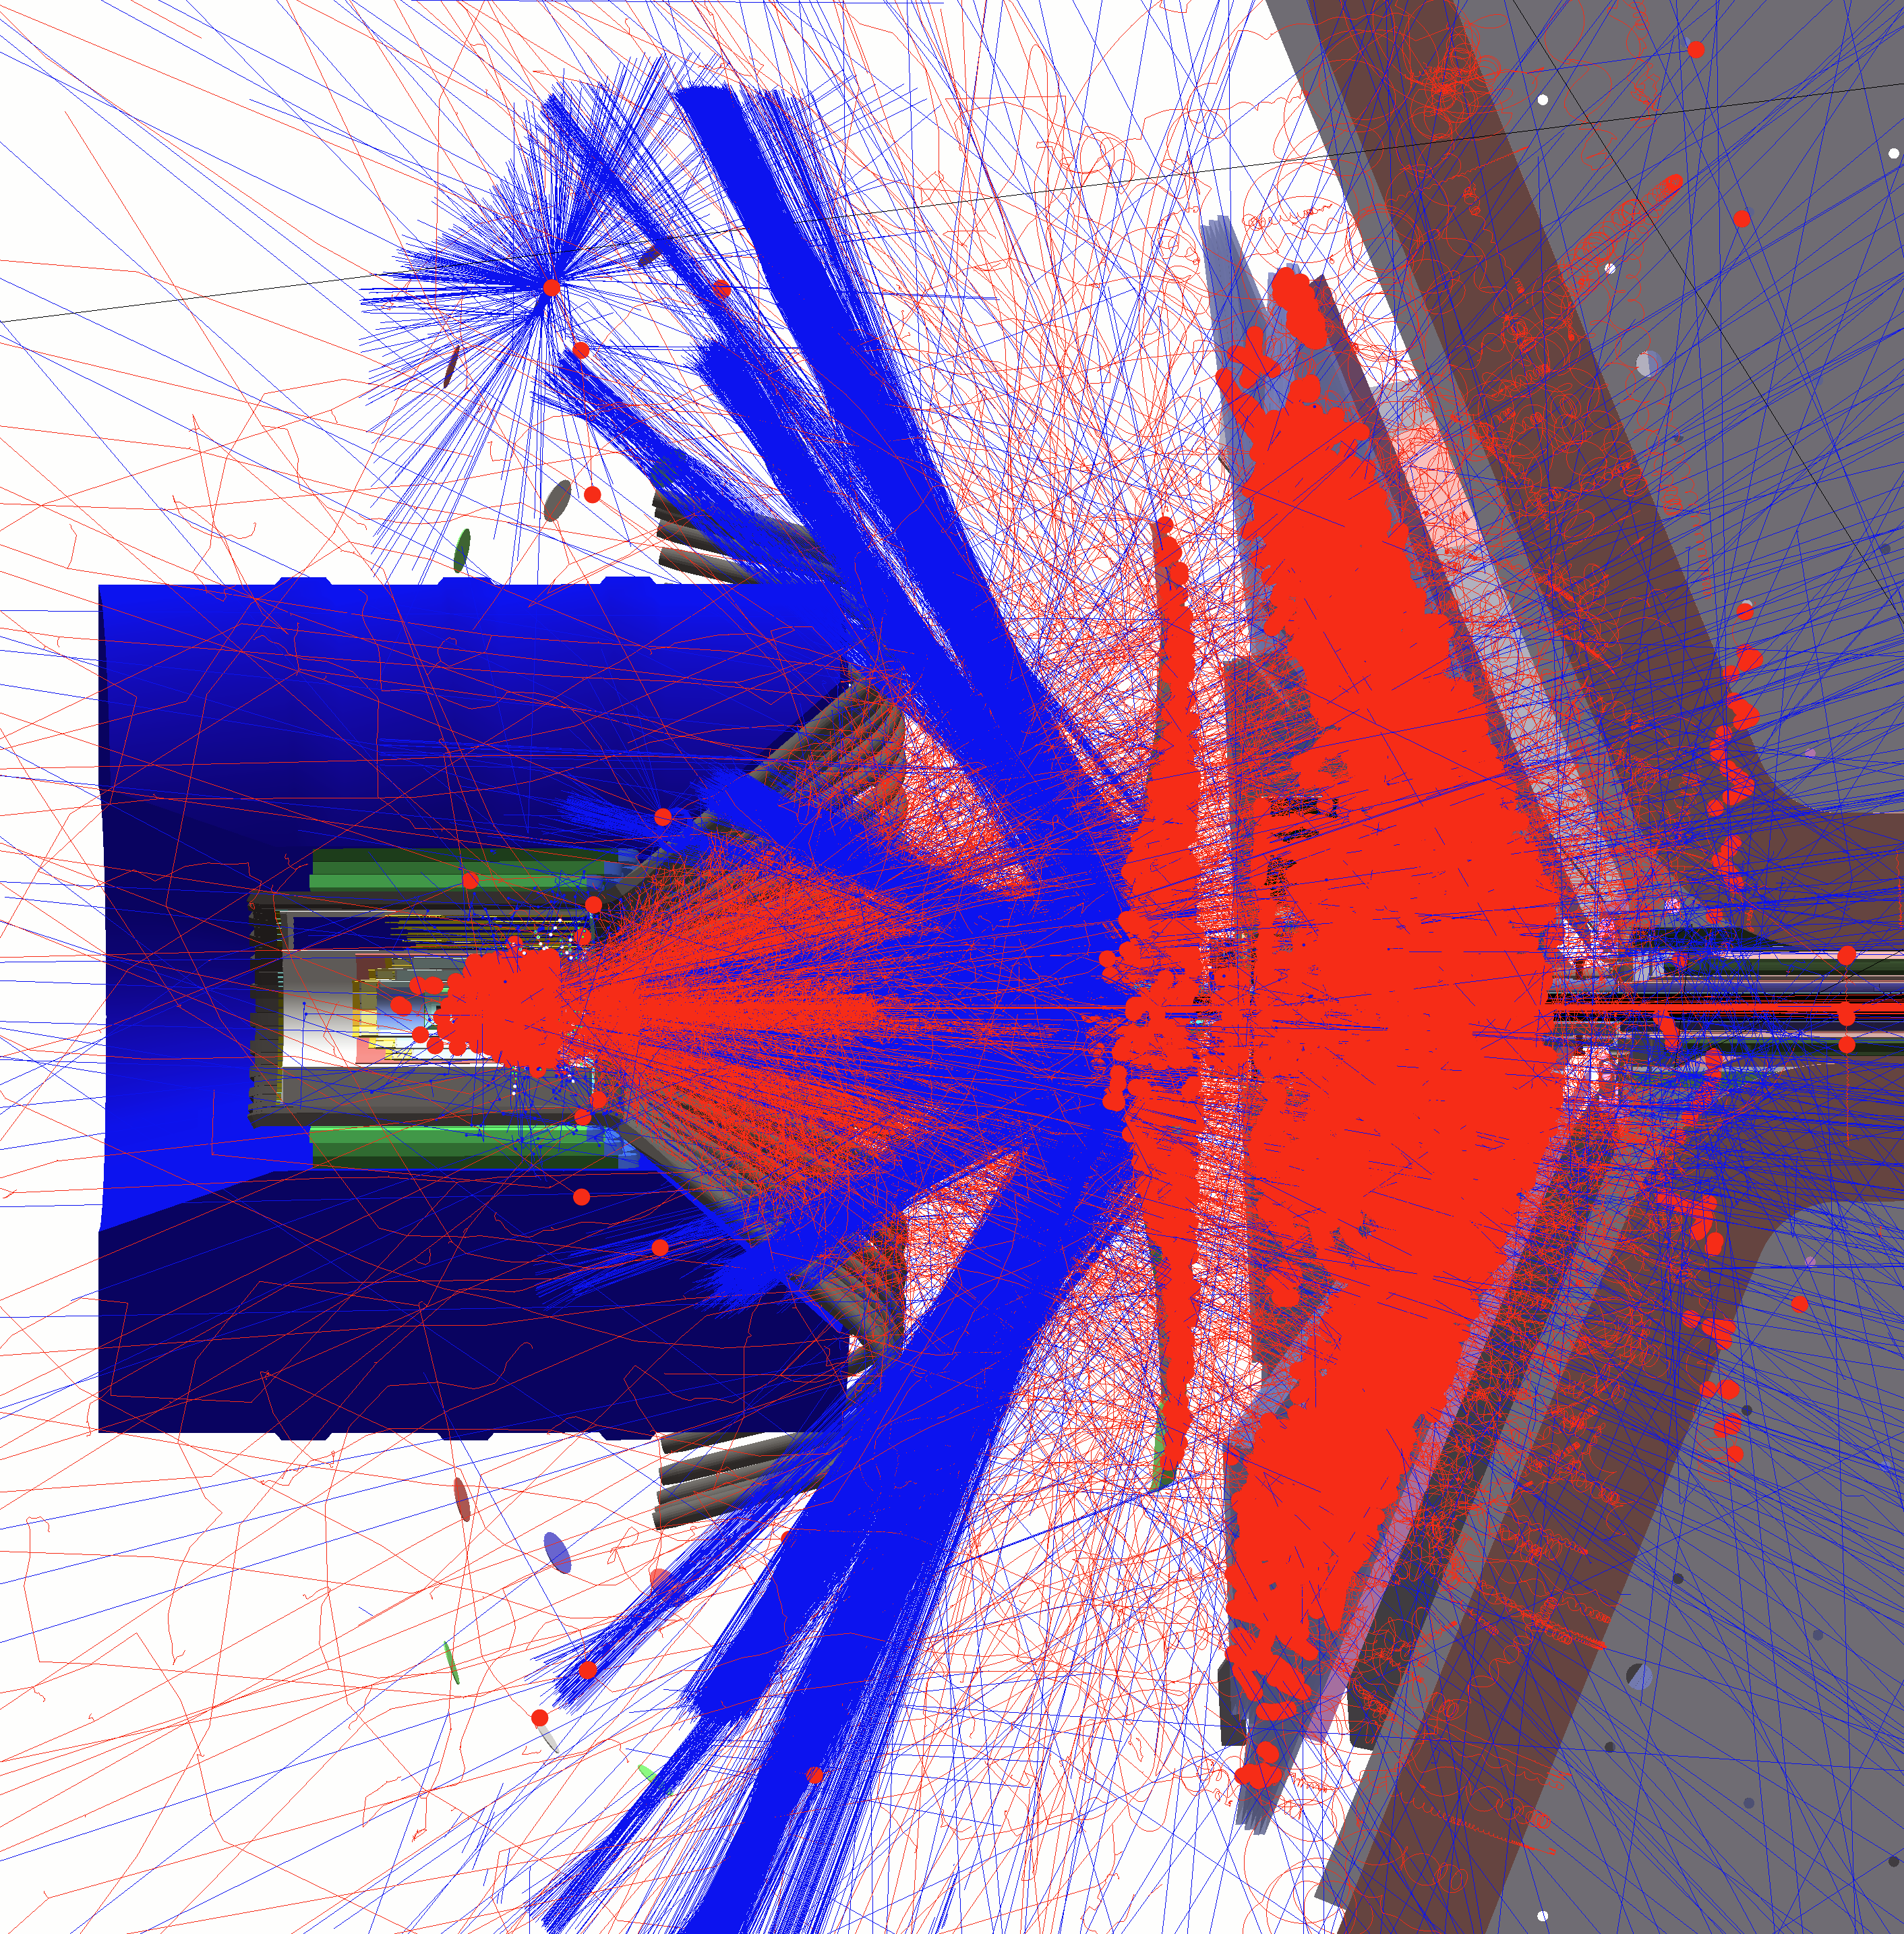
\includegraphics[width=1.0\columnwidth, height=1.0\columnwidth]{NoSolenoidFullTorusCut2.png}
}
\caption{(Color Online) Geant4 representations of accidental background events occurring within a 250~ns time window at different
magnetic field configurations and 100\% of design luminosity. Top left: Solenoid field is OFF and Torus field is OFF. Top
right: Solenoid field is OFF and Torus field is ON. Bottom: right Close-up of Top: right.  Bottom left: Solenoid field is ON
and Torus field is ON at 100\% design luminosity. Color code: red lines: primary electrons; red circles: hits in detectors; blue lines:
photons. }
\label{gemc-event}
\end{figure*}


Track reconstruction in the FD begins with hits in the drift chamber cells that can be connected to define a 
hit-based track, when at least 4 out of 6 layers in each super layer have hits, and in at least 5 out of 6 super layers. The
timing information is used to determine a time-based track and the particle momentum and flight path, while the TOF
gives the particle velocity ($\beta$) when combined with flight-path information. The momentum and velocity information
are combined to give the particle mass: $m = p/\beta\gamma$. Electron identification additionally requires the track to
match in time and position with both an HTCC hit and an isolated shower in the ECAL. The energy of the shower must be
consistent with the track momentum measured by the drift chambers in the Torus magnetic field.  

Charged particles are tracked in each sector separately using the 3 regions of drift chambers in each sector. Most
tracks are confined within one sector as the magnet optics and the massive mechanical support of the Torus coils
prevent most tracks from crossing from one sector into a neighboring sector. In rare cases low momentum charged
pions can cross from one sector into the opposite sector traversing through the beam pipe. Such tracks are not
reconstructed but they are included in the event simulation. Distributions of charged particles in azimuthal angle
versus momentum are shown in Fig.~\ref{neg-tracks}. Figure~\ref{vertex} shows the production vertex as reconstructed
in the FD tracking system (from data where the FMT was not installed). 

Neutral particles are detected in either the calorimeters or in the FTOF (or both). The reconstruction begins by finding
isolated clusters of energy, and determining the spatial location, deposited energy, and the time of the cluster. Neutral
particle candidates are identified as clusters in the outer detectors (FTOF, PCAL, EC) that do not match any charged
particle track. For high-energy photons that deposit all of their energy in the calorimeters, the energy is calculated from
the signal pulse height in the calorimeters. The momenta of neutrons are computed from their flight time as determined
by the timing signal in the calorimeters and, when relevant, the matched FTOF counter. In either case, the angle of the
neutral particle trajectory is determined from the position of the cluster at a depth in the ECAL that minimizes
parallax effects associated with tracks that are not normal to the face of the ECAL (see Ref.~\cite{ECAL} for
details).

For all events, precise determination of the interaction time or event start time is required. For events where the
scattered electron is detected, the event start time is derived from arrival time of the electron at the FTOF counters, 
corrected for flight path and signal delays.  The average time resolution for electrons reconstructed in CLAS12 FD is
better than 80~ps. A more accurate event start time is obtained by replacing the measured electron start time with the
499 (249.5)~MHz accelerator RF signal that determines the beam bunch associated with the event. In this way, the event
start time can be determined to within a few ps, thus eliminating a significant contribution to the time resolution for
charged hadrons. This extends the charged particle identification capabilities of CLAS12 towards higher particle
momentum.

Track reconstruction in the CD is generally less complex as tracks are determined fully by the geometry of the 
detection elements and the hit pattern in the CVT, i.e. by a combination of the SVT and the the BMT trackers. 
In contrast to the charged particle tracking in the FD that relies heavily ion timing information for resolution, 
this is not the case for the CD. In principle that makes tracking easier in the CD. On the other hand, the redundancy 
of track fitting is much reduced in the CD there are only 12 tracking layers compared to the 36 in the FD. This 
makes tracking in the CD more susceptible to losing tracks due to accidental hits. Particle identification in the CD is
limited to timing information in the CTOF scintillators combined with the track momentum measured in the strong solenoid 
magnetic field.  

See Ref.~\cite{Software} for full details on the CLAS12 offline reconstruction software architecture and design.


\subsection{Monte Carlo Simulations} 
\begin{figure}[t!]
\centerline{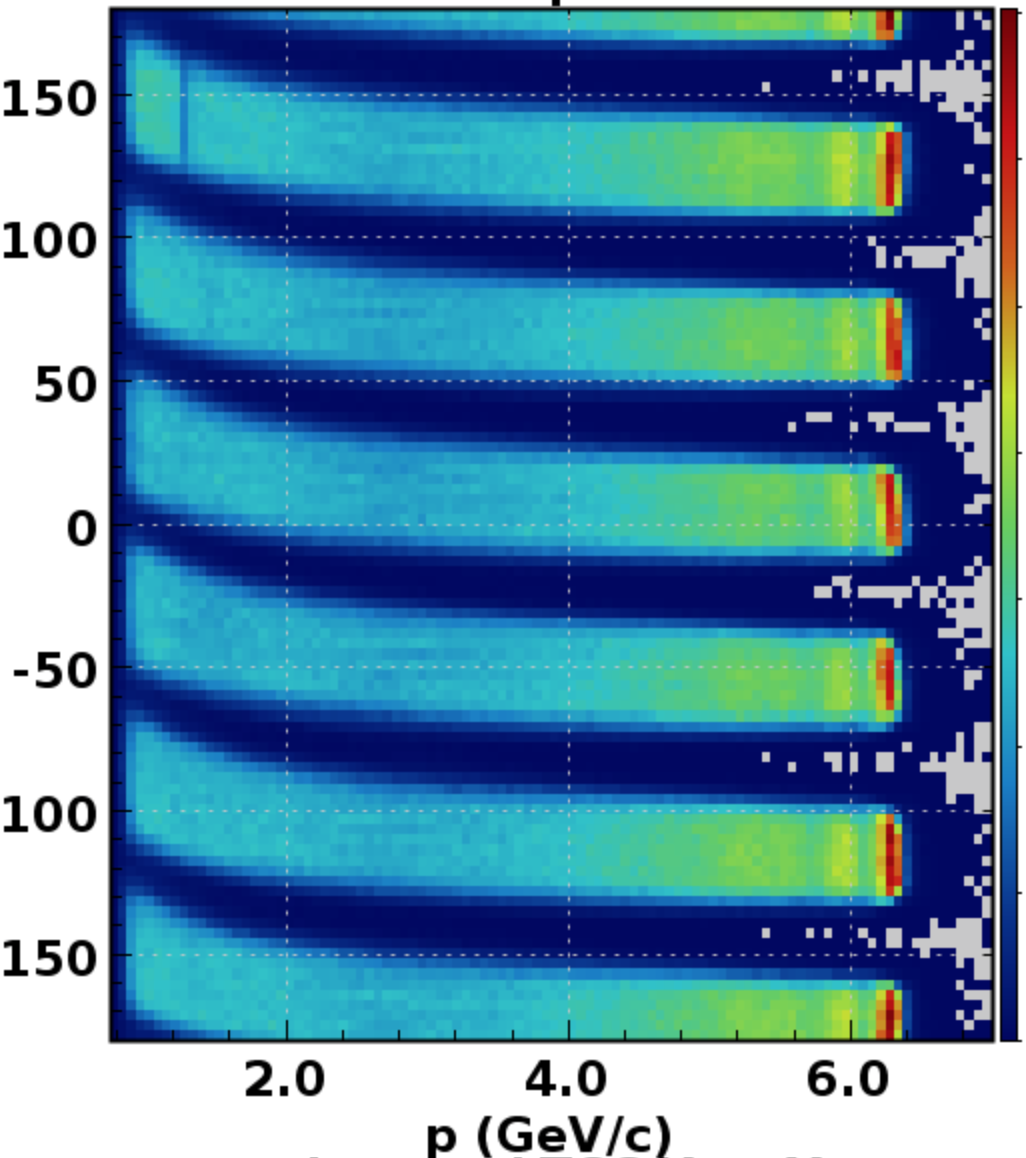
\includegraphics[width=0.9\columnwidth]{neg-tracks.png}}
\vspace{0.3cm}\centerline{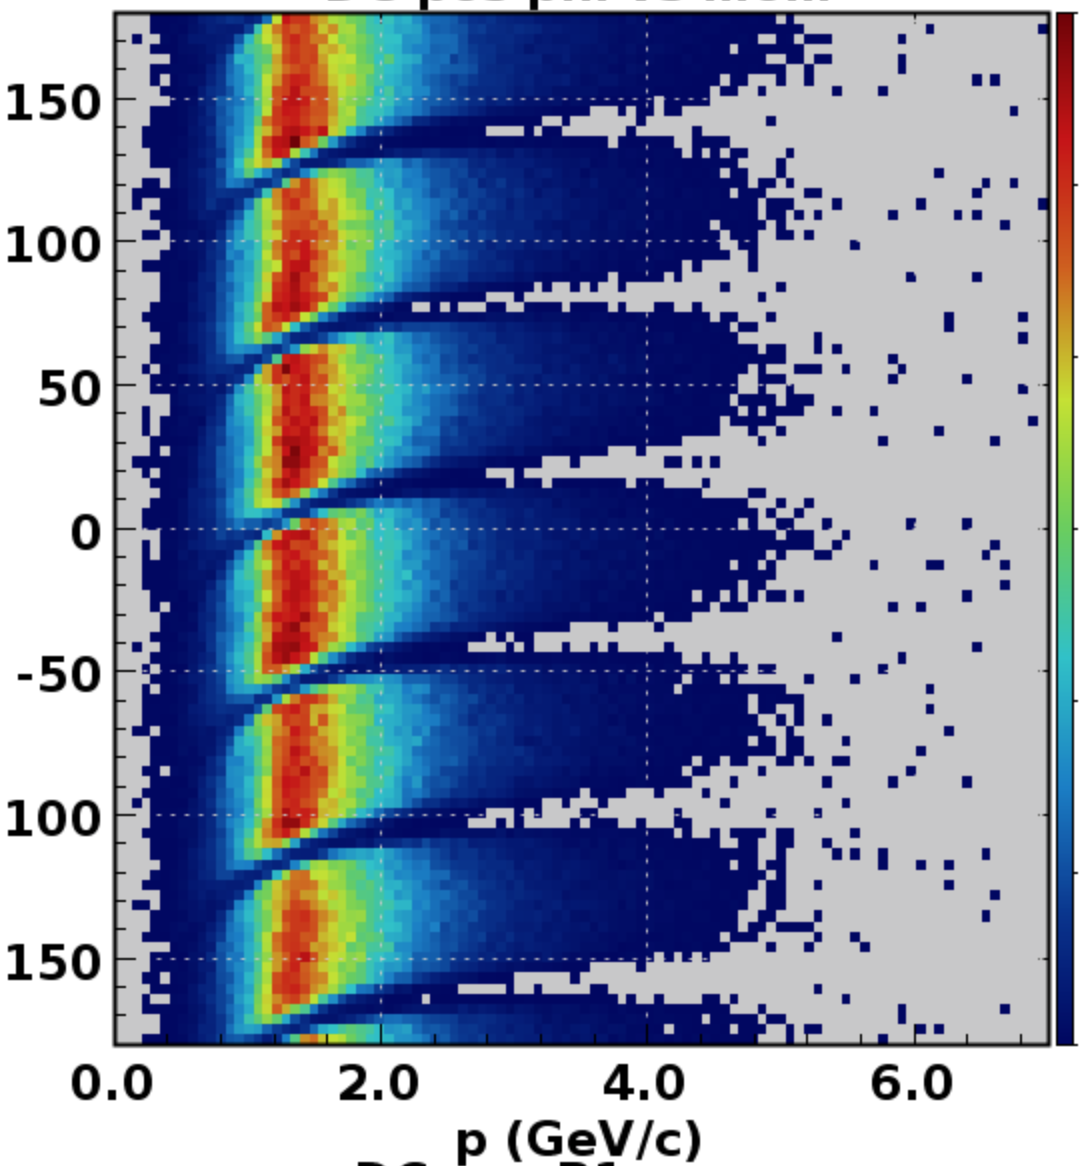
\includegraphics[width=0.9\columnwidth]{pos-tracks.png}}
\caption{(Color Online) Azimuthal angle acceptances versus momentum in the CLAS12 FD for negative (top) and for 
positive (bottom) tracks. The azimuthal angle is measured at the production vertex. The momentum dependence 
is due to the solenoidal magnetic field that rotates charged tracks dependent on their transverse momentum component and charge.
For positive tracks the azimuthal motion is in the opposite direction from negative tracks.} 
\label{neg-pos}
\end{figure}

\begin{figure} 
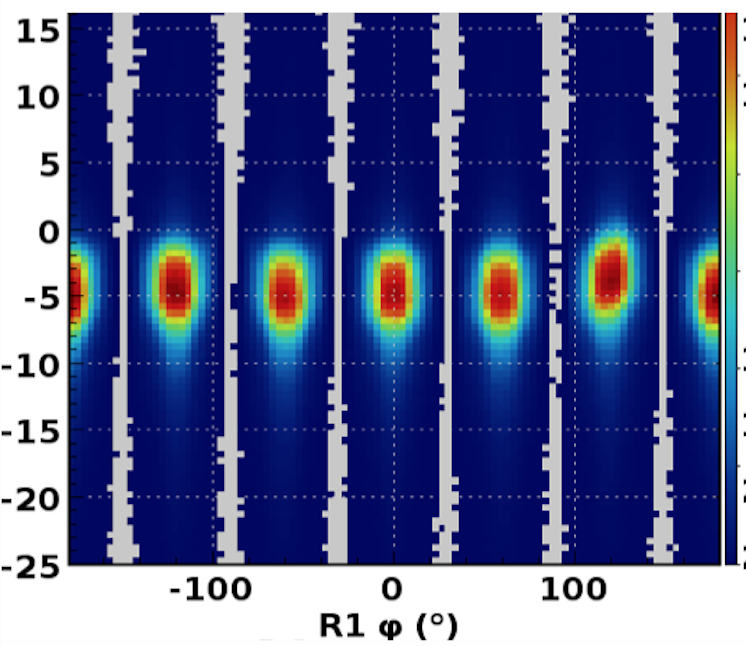
\includegraphics[width=0.9\columnwidth]{R1-vertex.png}
\caption{(Color Online) Electron vertex reconstruction in the FD versus azimuthal angle, before tracing the electrons 
back through the solenoid field. In this view tracks entering different Torus magnet sectors are not mixed. The target cell 
has a length of 50~mm .} 
\label{vertex}
\end{figure}

A critical part of operating an open large-acceptance detector system at high luminosities is the simulation not only of
hadronic events but also, and more importantly, the simulation of the beam-related accidental hits in the tracking system.
The source of accidentals is primarily from the beam electron elastically scattering off atomic electrons (M{\"o}ller
electrons) and their secondary interaction with beamline components. The production rate is orders of magnitude larger
than the hadronic production rate. These background sources have to be shielded through careful design of magnetic
channeling, as well as a proper design of the beamline shielding and the vacuum pipe to minimize interaction of these
electrons with high-$Z$ material. The availability of a realistic simulation package was essential for the optimal design
of the CLAS12 integrated detector concept. The strong solenoid field is essential in channeling the scattered M{\"o}ller
electrons through the beam enclosure to avoid interactions with the beamline materials. Figure~\ref{gemc-event}  shows
a single electron track event at 1/30 of the full luminosity in a time window of 250~ns, corresponding to the readout time
window in the R1 drift chambers. 
 
Additionally, a realistic simulation package is essential for the normalization of cross sections, especially to take into
account the detector occupancies for data taking at luminosities near or above the maximum design luminosity where the
track reconstruction efficiency can be significantly affected by accidentals. In order to quantitatively account for this,
data were taken at different beam currents (i.e. different luminosities) with randomly triggered events. Data from these 
randomly triggered events were merged with simulated physics events to study the loss of real tracks for different 
data runs. See Ref.~\cite{GEMC} for details on the CLAS12 simulation package GEMC.



\begin{figure}[t!]
{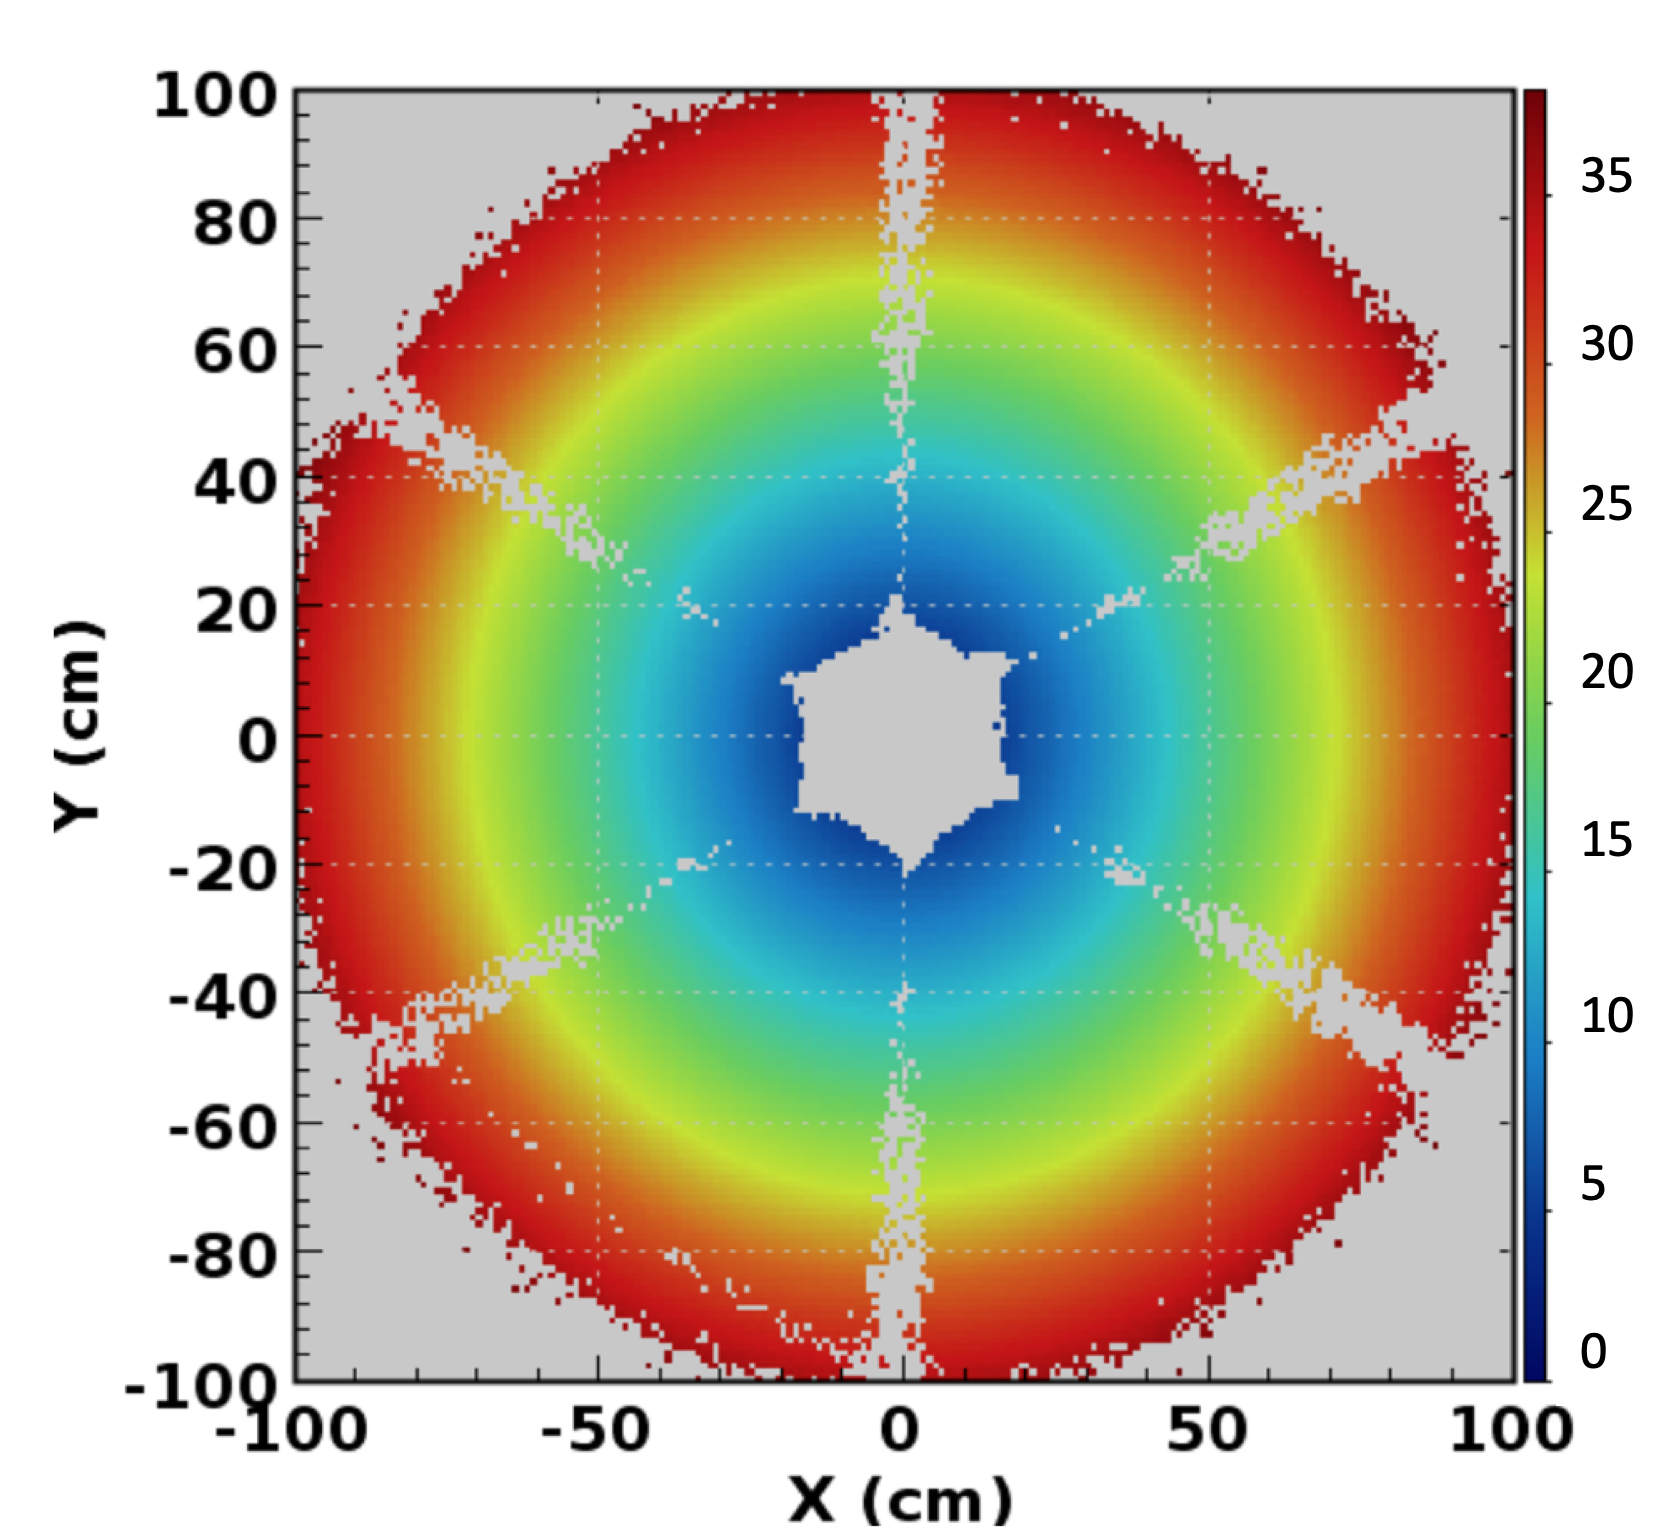
\includegraphics[width=1.0\columnwidth]{htcc-dis.png}}
\caption{(Color Online) Distribution of electrons at the HTCC location in polar and azimuthal angle. Bin sizes increase with
increasing polar angles. The gaps between sectors are not die to inefficiencies of the HTCC detector, but the result
of scattered electrons being lost in the Torus coils.} 
{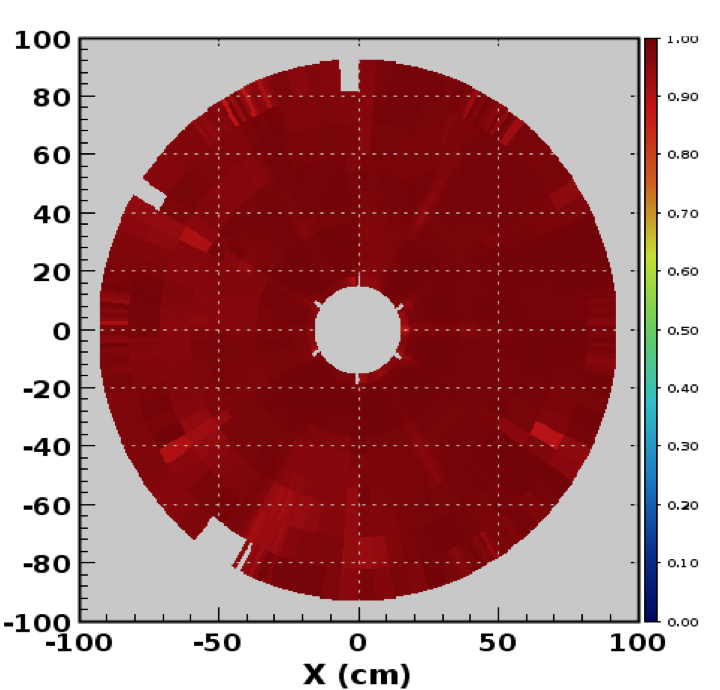
\includegraphics[width=0.96\columnwidth]{htcc-eff.png}}
\caption{(Color Online) Distribution of HTCC efficiencies in polar and in azimuthal
angles. The electron detection efficiency on average is greater than 98\% in the full phase space covered by the HTCC.
In localized areas, in particular at interfaces of different mirror facets or between mirror sectors efficiencies may vary from 95\% to 99\% } 
\label{htcc-eff}
\end{figure}

\section{CLAS12 Operational Performance}

This section describes the overall performance of the CLAS12 detection system. Most of the experimental programs
require the clean identification and reconstruction of the scattered electron. Electrons are identified by a combination
of signals in the HTCC and energy deposited in the combined electromagnetic calorimeters PCAL and EC and a negative
charged track in the drift chamber tracking system. Of critical importance is the response of the HTCC that operates
between the CD and the entrance to the drift chamber system. Figure~\ref{htcc-eff} shows the distribution of the
number of photoelectrons and efficiency in the 48 segments of the HTCC that cover the entire azimuthal angle range. 
The coordinates of the reconstructed electrons at the front face of the PCAL is shown in Fig.~\ref{electrons-xy}. The
distribution is rather uniform in all six sectors showing that the detector systems and the reconstruction software are
working properly. Elastic scattering  of electrons on protons allows for the establishment of any deviations from the ideal
detector geometry and alignment. The coverage in kinematical quantities $Q^2$ and $x_B$ of the scattered electrons
detected in the FD are shown in Fig.~\ref{electron-acceptance}. $Q^2$ is the virtuality of the photon exchanged from
the electron to the proton target and $x_B$ is the Bjorken scaling variable.

\begin{figure}[t!]
\centerline{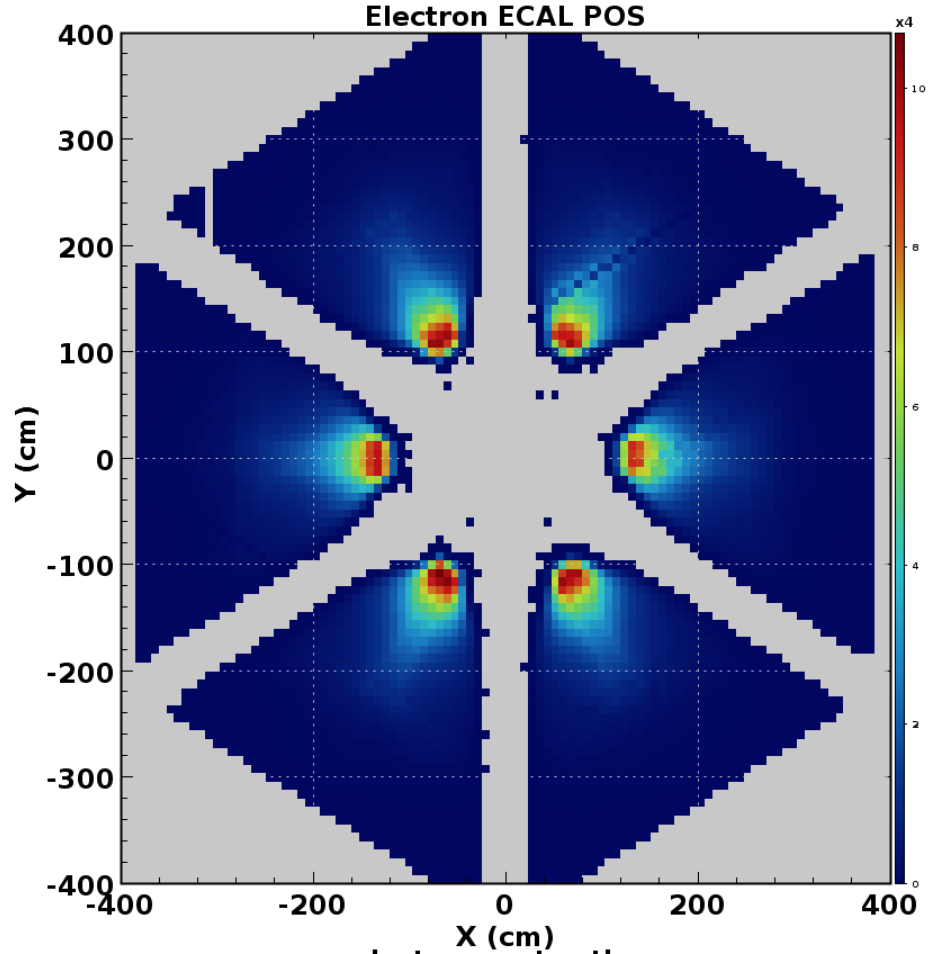
\includegraphics[width=1.0\columnwidth]{ElectronsOnPCAL.png}}
\caption{(Color Online) Distribution of electron track $x$ and $y$ coordinates propagated to the ECAL front face. The empty strip 
in the upper left sector results from a hardware issue. {\bf DO IT IN LOG SCALE?}} 
\label{electrons-xy}
\end{figure}

\begin{figure}[t!]
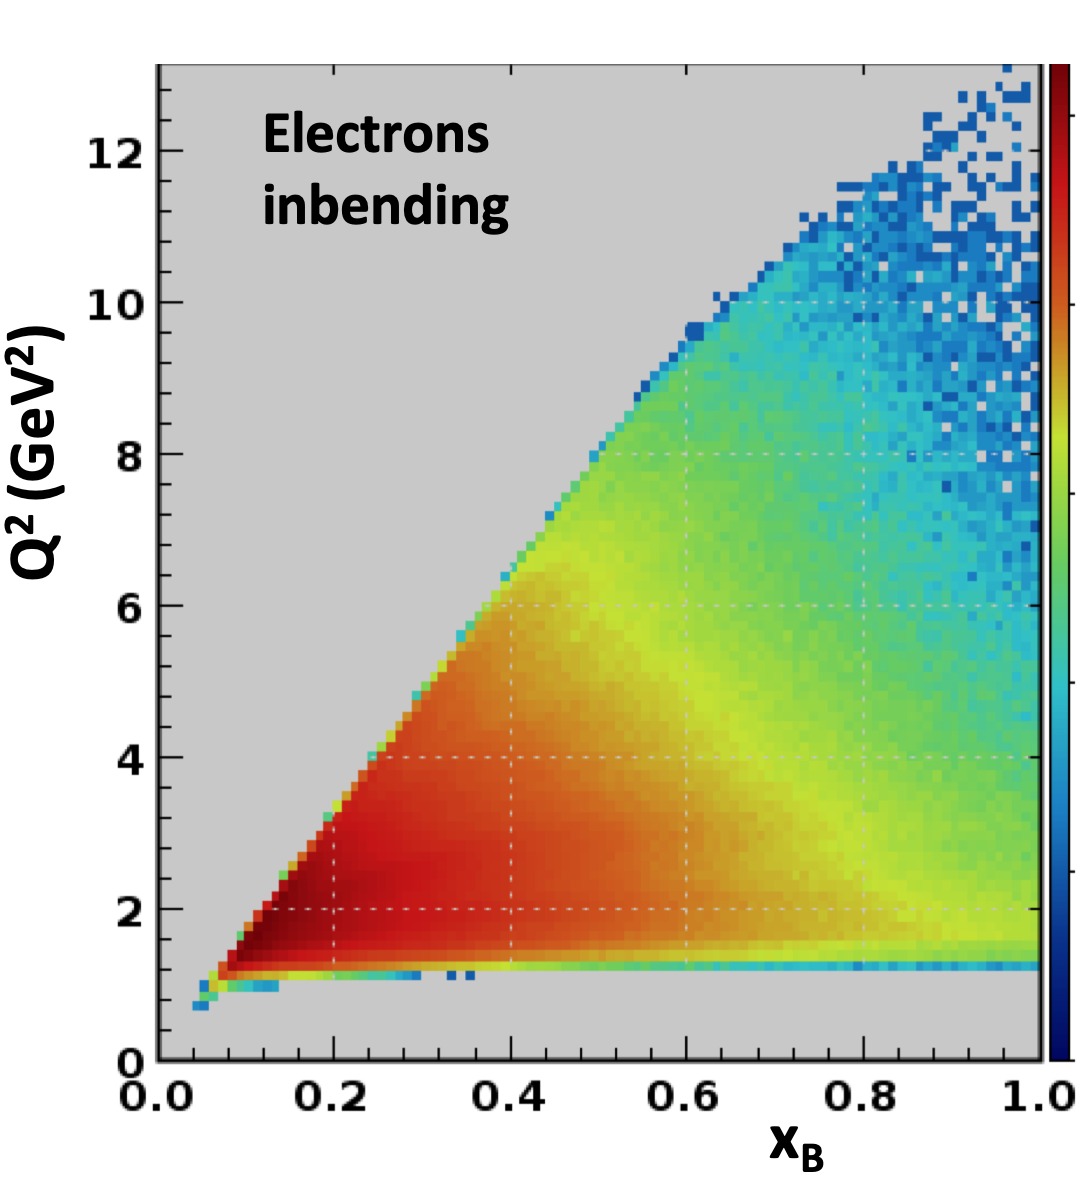
\includegraphics[width=0.97\columnwidth]{epX-in.png}
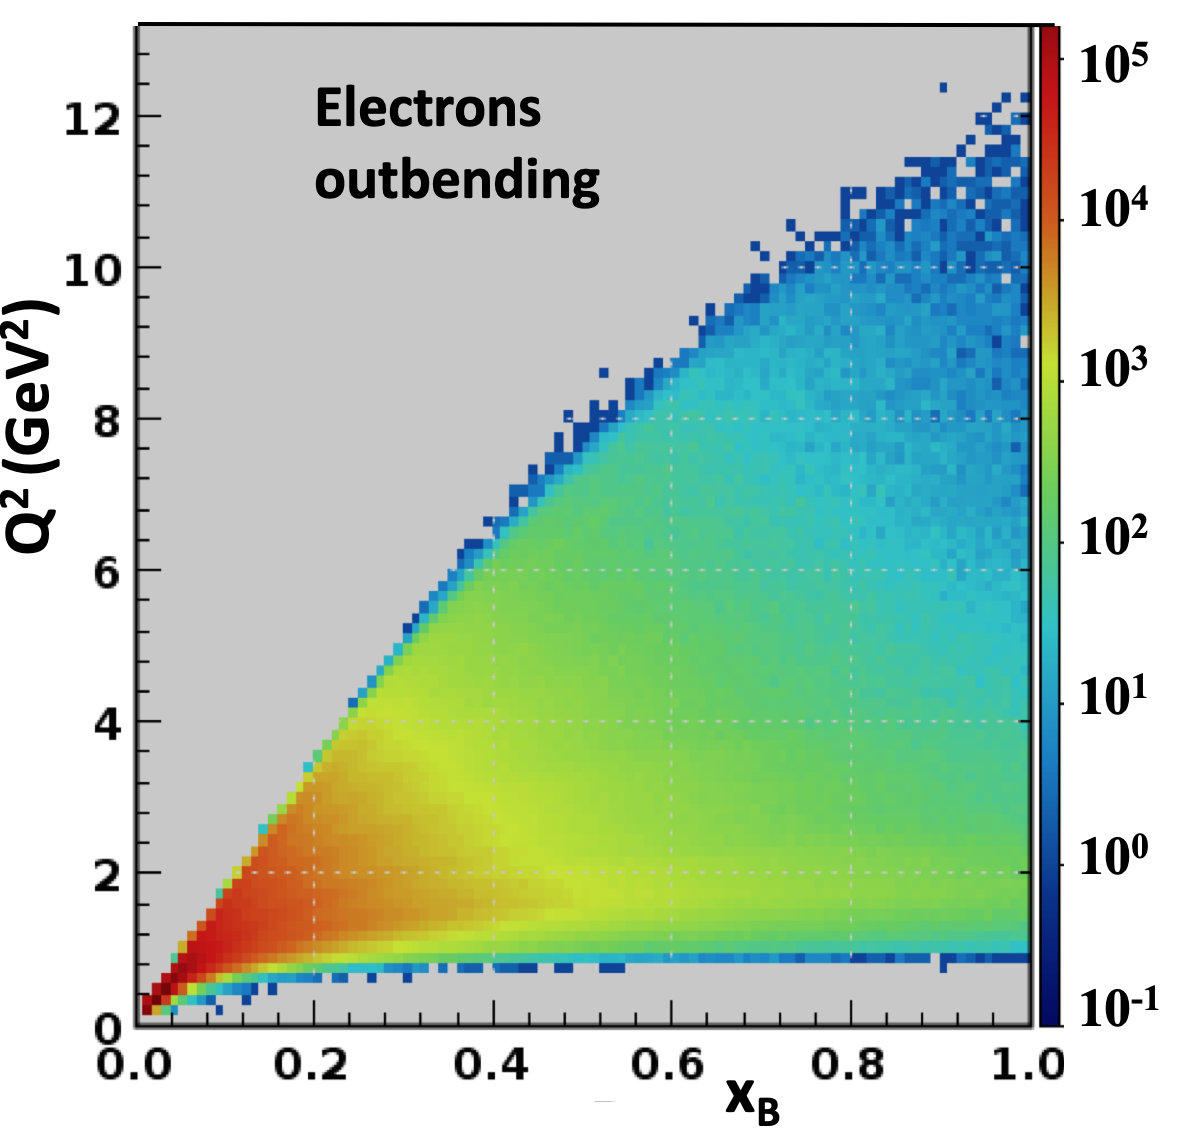
\includegraphics[width=1.0\columnwidth]{epX-out.png}
\caption{(Color Online) Inclusive $ep \to e'X$ coverage in $Q^2$ vs. $x_B$ at a beam energy of 10.6 GeV. 
The full kinematics is measured simultaneously. The
kinematic range is given by the beam energy to the left, the elastic scattering kinematics at $x_B = 1$, and the
small angle acceptance at the $Q^2$ limit for scattered electrons bending towards the beam line (in-bending) or away from the 
beam line (out-bending). The two configurations require opposite directions of currents in the Torus magnet coils.
Note that the minimal $Q^2$ is lower for the electron out-bending configuration, and that the maximum $Q^2$ 
reach is slightly higher for in-bending electrons.} 
\label{electron-acceptance}
\end{figure}

\subsection{Charged Particle Detection in FD}
 
Charged particles acceptances in momentum and azimuthal angles are shown in Fig.~\ref{neg-pos} in the sector
frame for positively and negatively charged particles. The difference in the acceptance is due to two factors, the
polarity of the Torus magnet that bends negative particles away from the beam line and positive particles towards
the beamline, and the effects of the solenoid magnetic field that causes an azimuthal motion for positive and negative
particles in opposite directions. 

\begin{figure}[htbp!]
%\centerline{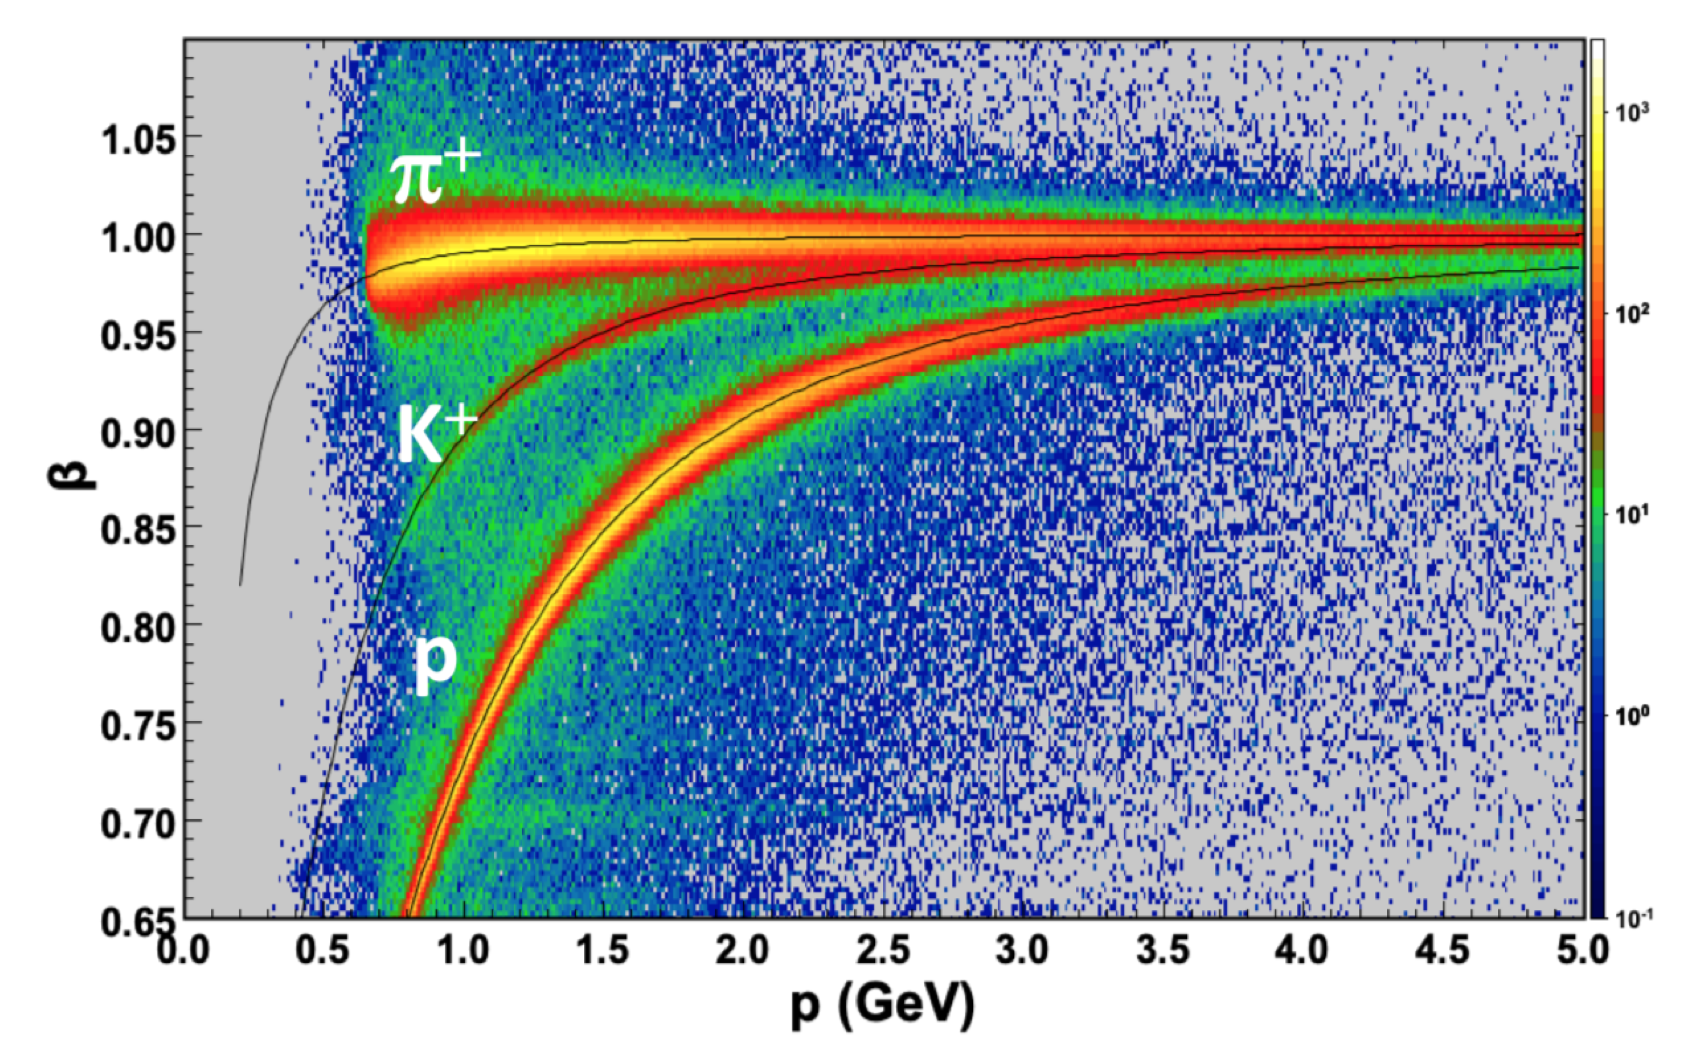
\includegraphics[width=1.1\columnwidth]{FTOF1b_pid.png}}
\centerline{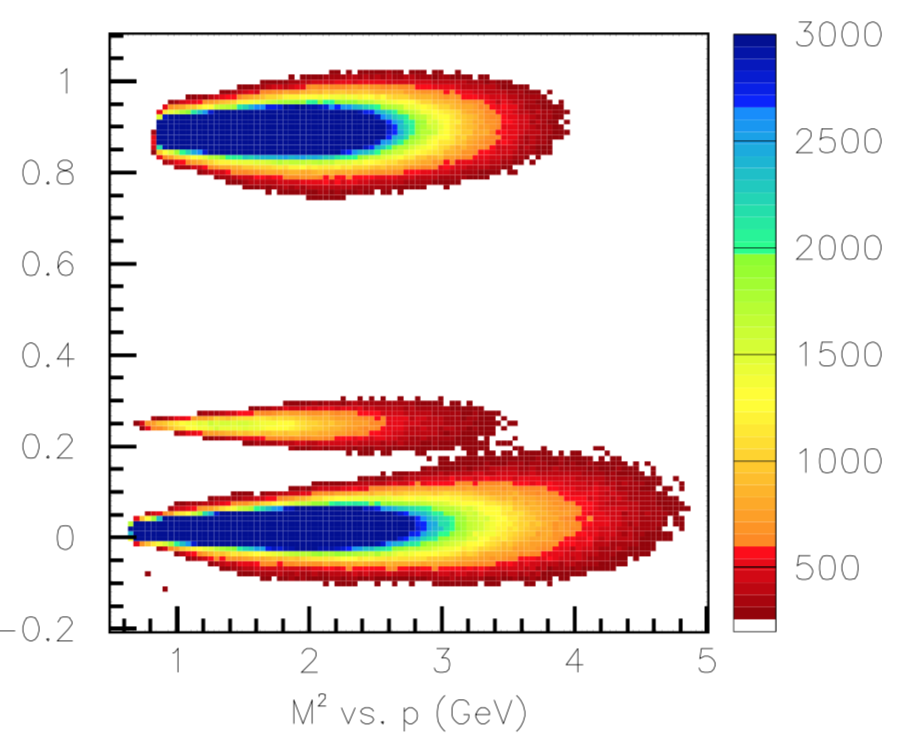
\includegraphics[width=1.1\columnwidth]{FTOF1b_M2-vs-p.png}}
\caption{(Color Online) Velocity $\beta = v/c $ versus momentum of positively charged particles detected in the CLAS12 FD. The
thin black lines show the expected distributions for the respective charged tracks. Particle identification is limited
to momenta greater than 0.8~GeV when the Torus magnet is energized to maximum current. At reduced current the
tracking is extended to lower momenta at the expense of momentum resolution.}
\label{pid}
\end{figure} 

Identification of charged particles in CLAS12 is achieved in a number of ways. Identified electrons are used to
determine the start time of hadrons at the production vertex. The start time and the path length of charged tracks
from the production vertex to the FTOF and the arrival time enable determination of the $\beta = v/c$ of the
particle, shown in Fig.~\ref{pid} versus particle momentum for positive charged tracks and the mass projections are
shown in Fig.~\ref{pid-1D}.  An overview of the particle identification in the various CLAS12 detector systems vs.
momentum is given in Fig.~\ref{pid1}. 

\begin{figure}[htbp!]
\centerline{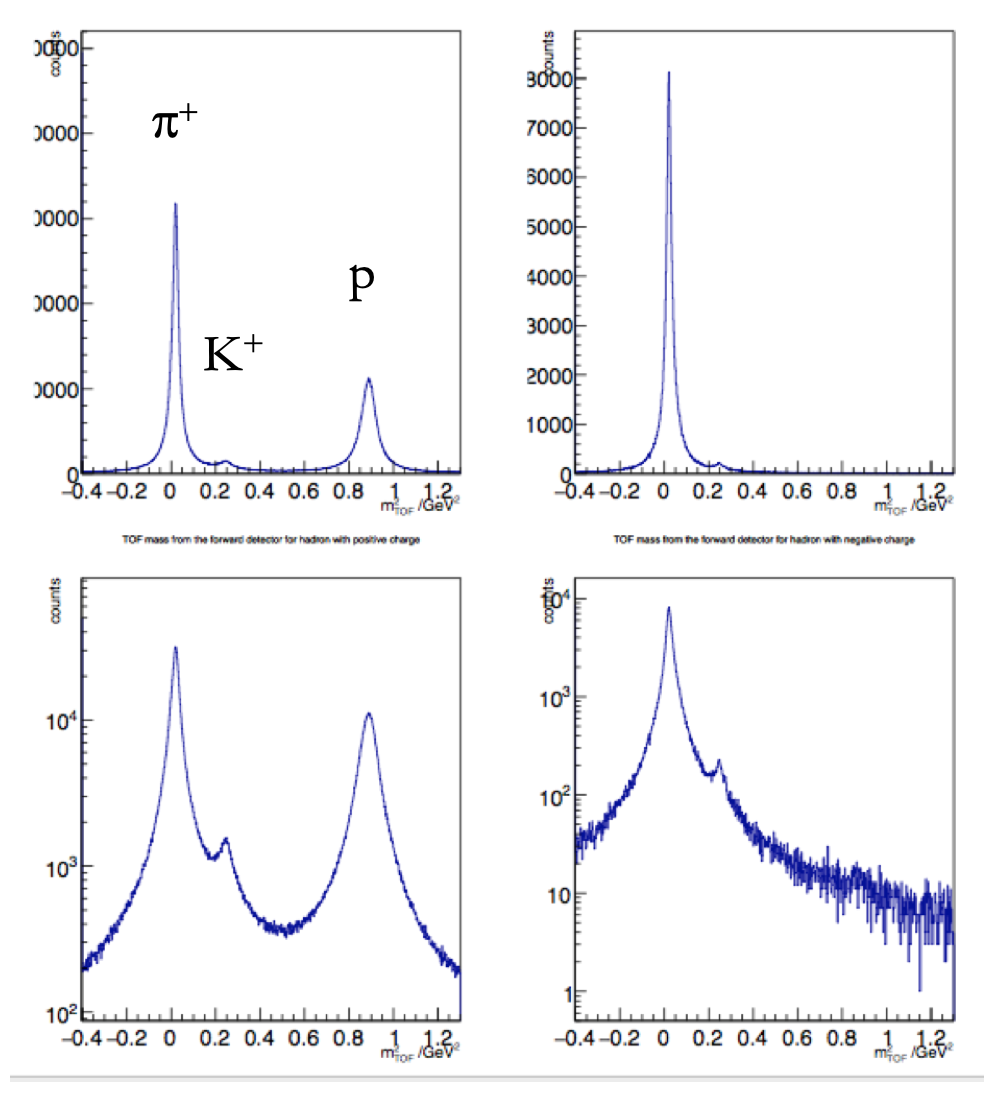
\includegraphics[width=1.0\columnwidth]{pid-1d.png}}
\caption{{$\rm Mass^2$} of charged particles evaluated from their momentum and the time-of-flight information
in the FTOF. Left: Positively charged hadrons: $\pi^+$, $K^+$, $p$. Right: Negatively charged hadrons: $\pi^-$,
$K^-$, ${\bar{p}}$. {\bf Clean up plots for publication.}}
\label{pid-1D}
\end{figure} 

\begin{figure}[htbp!]
\centerline{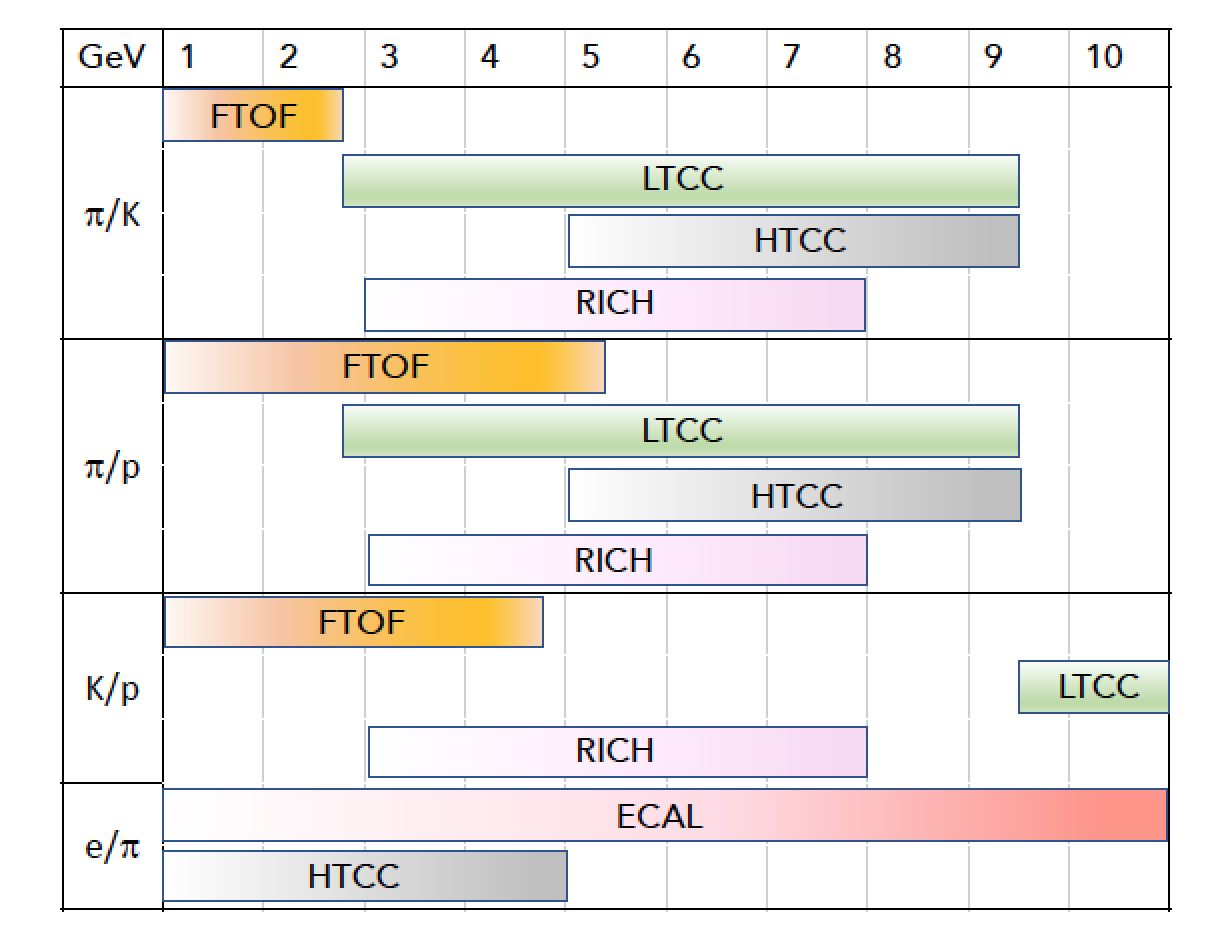
\includegraphics[width=1.1\columnwidth]{CLAS12-pid.png}}
\caption{(Color Online) Overview of particle identification in various detectors of the CLAS12 FD. The higher (lower) intensity
of the color shading indicates higher (lower) effectiveness for the particle species separation shown.} 
\label{pid1}
\end{figure} 

Figure~\ref{spectrum} shows the inclusive spectrum $ep \to e' X$ and the $ep \to e' \pi^+ X$ with a missing
neutron at four different beam energies. Figure~\ref{elastic-peak} shows fits to the elastic peak and to the
missing neutron mass distributions in three sectors at a beam energy of 10.6~GeV. Figure~\ref{pip-pim-p} shows
the invariant mass of $\pi^+\pi^-$ and the missing mass $M_X$ for the reaction $ep \to e' \pi^+ \pi^- X$.  

\begin{figure*}[ht]
\centerline{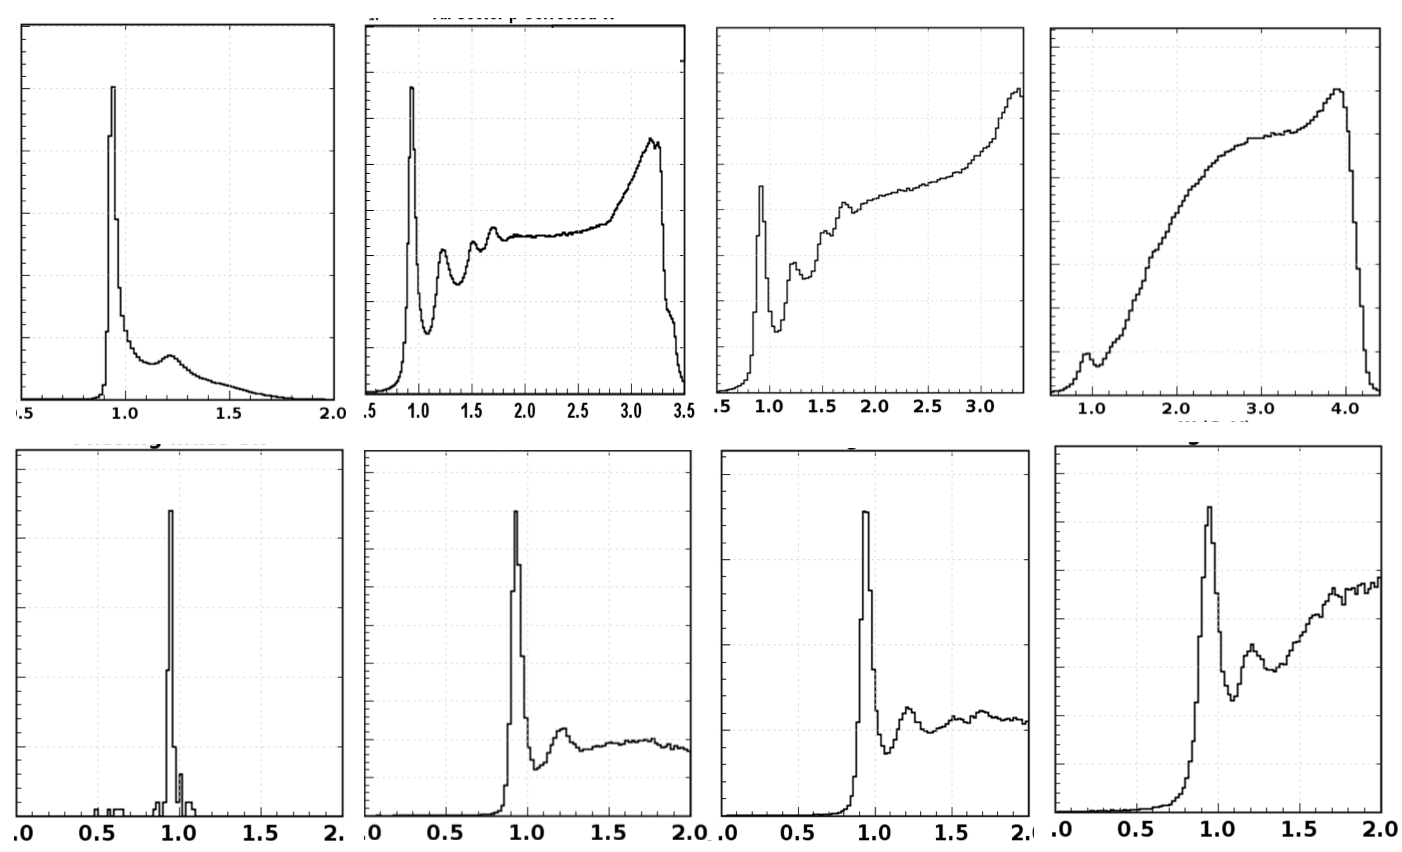
\includegraphics[width=1.8\columnwidth]{W-spectrum.png}}
\caption{Upper row: Inclusive electron scattering spectrum $ep \to e' X$ measured in CLAS12 at beam energies 
of 2.2~GeV, 6.5~GeV, 7.5~GeV, and at 10.6~GeV (from left to right). The peak to the left is due to elastic $ep \to ep$
scattering. Enhancements from the first 3 excited nucleon states, $\Delta(1232)$, $N(1520)$, and $N(1680)$, are also
visible for the lower beam energies. Note that the mass ranges  are different for the different beam energies. Lower
row:  Missing mass distributions of $ep\to e' \pi^+X$ for the same energies. The sharp mass peak to the left is due
to the undetected neutron. The second peak for the higher energies is due to the $\Delta^0(1232)$. Indications of higher
mass neutron excitations are also visible. The horizontal axes are in units of GeV. } 
\label{spectrum}
\end{figure*} 

\begin{figure}[t!]
\centerline{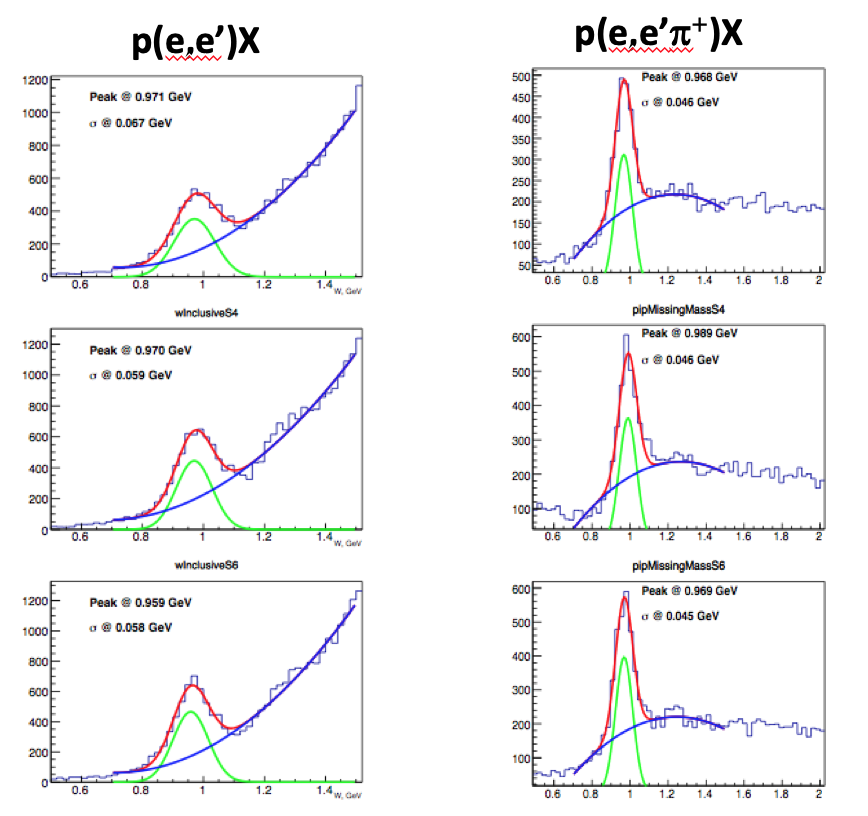
\includegraphics[width=1.0\columnwidth]{elastic_pi+n.png}}
\caption{(Color Online) The left panels show the elastic peak at 10.6~GeV beam energy as measured in 3 representative sectors. The
peak is close to the proton mass in all sectors reflecting the good momentum calibration of all sectors. A fit to the
elastic signal shows sector to sector variation of less then {\bf XX MeV} ({\bf need to replace after kinematic
corrections have been applied}). The right panels show the mass distribution of the unmeasured final state X in
$ep \to e'\pi^+ X$. The missing mass peak is due to the unmeasured neutron. {\bf Replace after kinematic corrections are applied.}
The mass resolution is $\sigma_X = 45$~MeV/c$^2$. {\bf Clean up plots for publication.}} 
\label{elastic-peak}
%\end{figure} 

%\begin{figure}[htbp!]
\vspace{0.3cm}\centerline{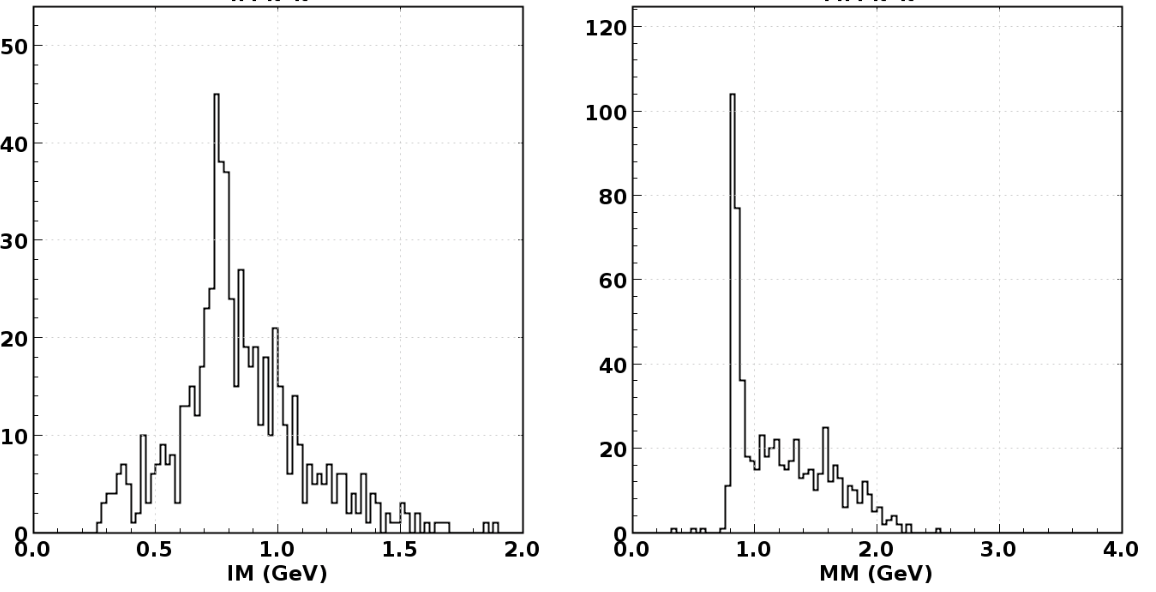
\includegraphics[width=1.0\columnwidth]{pip-pim-p.png}}
\caption{Left: Invariant mass of $\pi^+\pi^-$, showing the peak at the $\rho^0$ mass. Right: missing mass 
$M_X$  of $e'\pi^+\pi^-X$ with the peak at the proton mass that establishes the exclusive process
$ep\to e' p \pi^+\pi^-$. ({\bf waiting for better statistics after cooking)}}
\label{pip-pim-p}
\end{figure} 

\subsection{Charged Particle Detection in CD} 

Momentum reconstruction in the CVT combined with the timing information from the CTOF allows for the separation 
of charged pions from charged kaons and from protons in the momentum range from 0.25~GeV to 1.25~GeV. The momentum
range covers a large part of the phase space allowed by the maximum beam energy for hadron electro-production 
on hydrogen targets. Figure~\ref{CD-PID} shows the particle velocity $\beta = v/c$ versus the particle momentum 
reconstructed in the CVT.

\begin{figure}[t!]
\centerline{\includegraphics[width=1.0\columnwidth]{CTOF-pid-new.png}}
\centerline{\includegraphics[width=0.8\columnwidth]{CTOF-mass.png}}
\caption{(Color Online) Top: $\beta$ measured in CTOF versus momentum measured in CVT of positively 
charged particle momentum in the CD. Bottom: Reconstructed $\rm mass^2$ for positively charged particles
 at 10.6~GeV beam energy. The peak to the left is due to $\pi^+$, the bump to the right is due to protons. 
 Momenta are not corrected to energy losses in the CVT.}
\label{CD-PID}
\end{figure} 

\subsection{Neutral Particle Detection} 

Direct detection of neutral particles is accomplished in the FD using the PCAL and EC calorimeters. The combined
20 radiation length is sufficient to identify high energy photons and reconstruct masses of parent particles, such
as $\pi^0\to \gamma \gamma$  or $\eta \to \gamma \gamma$. At very forward angles the FT provides photon
detection with significantly improved position and energy resolution in the polar angle range from 2.5$^\circ$ to
4.5$^\circ$. Figure~\ref{gg} shows the invariant mass of the $\gamma\gamma$ system in the CLAS12 FD and in
the FT calorimeter, respectively. 

\begin{figure}[htbp!]
\centerline{\includegraphics[width=0.95\columnwidth]{ECAL-2g-mass-fit.png}}
\caption{(Color Online): The invariant mass of two high-energy photons in sector 4 of the ECAL. The background beneath
the $\pi^0$ peak is due to multi-photon decays of higher mass mesons where one or more photons are not detected
in the angle range covered by the calorimeter. The widths of the mass peak is 11.9~MeV. The energy calibration of the calorimeter 
uses cosmic ray events. }
\centerline{\includegraphics[width=1.15\columnwidth]{FT-performance.png}}
\caption{Top panel: The energy response of the FT calorimeter to elastically scattered electrons at 2.2 GeV beam energy. 
The tail at lower energies is due to radiative effects. The energy resolution is $\sigma_E / E \approx 3.3\%$. 
Bottom panel: 2-$\gamma$ mass for photons detected in the FT lead-tungstate crystal calorimeter. The $\pi^\circ$ 
mass resolution is $\sigma_{\gamma\gamma} = 4.4$~MeV. }

\label{gg}
\end{figure}




Neutral particle detection in the CD is provided by the CND combined with the CTOF. The polystyrene plastic
scintillator bars of the two detectors have a combined 15\% nuclear interaction length resulting approximately in
a 12\% efficiency for the detection of high energy neutrons. The plastic scintillators contribute about 29\% of a
radiation length at 90$^\circ$ polar angles; they are also detecting high energy photons through their conversion
in $e^+e^-$ pairs. The discrimination of photons and neutrons in the CD is  accomplished by the timing resolution of
80~ps provided by the CTOF and the 150~ps of the CND. The separation of neutral particles from charged
particle hits in the CND or in the CTOF is efficiently achieved by using the CVT tracker to veto against false neutral
hits in the CTOF and CND. Figure~\ref{CND-neutrals} shows the velocity versus the energy deposition of charged
and neutral particles in the CND.  

\begin{figure}[htbp!]
\centerline{\includegraphics[width=0.9\columnwidth]{CND1.png}}
\centerline{\includegraphics[width=0.9\columnwidth]{CND2.png}}
\caption{(Color Online) Top panel: Distribution of $v/c$ for charged particles in the CND vs. the deposited energy for correlated
charged tracks in the CVT. Evidence for charged pions and protons is clearly visible.  Bottom panel: The same for
neutral particles; no charged tracks are correlated to the energy deposited in the CND scintillators. The cut at
$v/c$ = 0.2 eliminates background events from accidental hits. {\bf NEED BETTER GRAPHS}} 
\label{CND-neutrals}
\end{figure} 

\section{Data Acquisition and Trigger System} 

\subsection {CLAS12 Data Flow and Monitoring} 

During data taking the quality of the data is continuously monitored by displaying a very small fraction of single
events in the CLAS12 event display (ced) that allows immediate action by the shift personnel in case of obvious
issues. Monitoring histograms are filled on a regular basis that include simple analysis and can be easily compared
with histograms collected earlier during the data taking.  

The CLAS12 data acquisition (DAQ) is a dead-time free system designed for an average of 20~kHz level 1 (L1) 
trigger rate, pipelined and for continuous operation. The sector-based  L1 triggers support streaming, subsystem
hit patterns, and energy summing with low threshold suppression.  The scalable trigger distribution scheme uses up
to 128 front-end L1 crates. CLAS12 uses different programmable features for each detector that participates in
the L1 trigger. A schematic diagram showing a complete overview of the DAQ system is shown in Fig.~\ref{daq}. In
2018 the DAQ was run at trigger rates of typically 15~kHz and data rates of 500~MB/s with a live time of $> 95\%$.
At somewhat lower live time of $\sim$90\%, trigger rates of 20~kHz and data rates of up to 1~GB/s were achieved.
Details of the design, functionality, and performance of the CLAS12 DAQ are provided in  Ref.~\cite{DAQ}. 
 
\begin{figure}[htbp!]
\centerline{\includegraphics[width=1.0\columnwidth]{clas12-daq.png}}
\caption{(Color Online) Schematic diagram of the CLAS12 data acquisition and trigger system.}
\label{daq}
\end{figure}
\begin{figure}[t!]
\centerline{\includegraphics[width=0.95\columnwidth]{trigger.png}}
\caption{(Color Online) View of an event in CLAS12 from the ced event display. Predefined trajectories 
are employed to select hit
patterns in the 3 drift chamber regions that correspond with localized energy deposition
in the PCAL and EC. For the two-track trigger the two sectors show drift chamber hit patterns for tracks with
opposite charges. The upper track is an electron, shown by the hit in the HTCC, and bends towards the beam line, 
the lower one has positive charge and bends away from the beam line.}
\label{trigger}
\end{figure}
\begin{figure*}[t!]
\centerline{\includegraphics[width=2.0\columnwidth]{beamline-1.png}}
\centerline{\includegraphics[width=2.0\columnwidth]{beamline-3.png}}
\caption{(Color Online) Top: Hall~B beamline upstream of the target, showing the photon tagger magnet to the left, which is energized
during beam tuning and during polarization measurements. Further downstream is a doublet of beam raster magnets
that are used to raster the beam during polarized target experiments to avoid local polarization losses in the target.
The elements near the center are cavities for beam position and beam current measurements. The main element 
on the right is the solenoid magnet nearly fully encapsulated by the HTCC PMT housing. Several of the Torus magnet
coils are visible at the far right. 
Bottom: Hall~B beamline downstream of CLAS12 showing a shield wall at the left, a beam viewer, the beam blocker,
and the Faraday cup at the right. As the Faraday cup is not cooled, a cooled-copper 5-kW beam blocker is inserted
for 11~GeV beam operations above currents of 15~nA.}
\label{beamline}
\end{figure*}

\subsection{Fast and Selective Triggers} 

CLAS12 uses a series of fast triggers that are tailored to a specific event pattern selection. Most of the physics
experiments require the electron scattered on the production target to be detected as it defines the mass
($Q^2$) and kinematics of the virtual photon as $Q^2 = -(e - e')^2$, where $e$ and $e'$ are the 4-momentum
vectors of the beam electron and of the scattered electron, respectively. The electron kinematics also defines
the Bjorken scaling variable $x_B$  and the missing mass $W$ defined as $W^2 = M^2 + 2M\nu - Q^2$ with
$\nu = E_e - E_{e'}$, and $M$ the mass of the target particle. The scattered electron is uniquely identified with
signals in the HTCC, clustered energy deposition  in the PCAL and EC. To enhance section of specific reactions 
in the accumulated data, additional charged particles
in either the FD or the CD are selected in the trigger in addition to the scattered electron. The CLAS12 fast
trigger system makes use of the responses of the detectors to form the readout triggers. At the design
luminosity of CLAS12, the hadronic production rate is approximately $5 \times 10^6$/s. However, only a small
fraction of those events is of interest for the science program with CLAS12. In particular, most physics reaction
require the detection of the scattered electrons at some finite scattering angle, for example $\theta_{e'} > 5^\circ$.  
   
   

In some special programs the detection of electrons in the FT is of interest if they are associated with hadronic
event patterns of two additional detected hadrons. Such conditions have been implemented in the fast trigger
decision that reduces the number of triggers to about $2 \times 10^4$~events/s, i.e. by  a factor of 250 from the
hadronic rate. The data rate is typically 500~MB/s under such conditions and can be handled by the CLAS12 data
acquisition system and the available computing resources. Figure~\ref{trigger} shows one example of a hadron pair
trigger. It uses the drift chamber ``roads'' (amounting to hit patterns stored in look-up tables consistent with
charged tracks coming from the region of the target), associated signals and energy deposition in the
PCAL and EC that are consistent with two minimum ionizing particles. This trigger has a near 100\% efficiency and a
25\% purity. Another trigger is the inclusive electron trigger, which in addition to the hadron trigger makes use of
a correlated signals in the HTCC. Details of the design, functionality, and performance of the CLAS12 trigger are
provided in Ref.~\cite{TRIG}. 

 



\section{Electron Beam Operation} 

\subsection{Beamline}

The Hall~B beamline has two sections, the 2C line, from the beam switch yard (BSY) to the Hall proper, and the 2H
line, from the upstream end of the experimental Hall to the beam dump (or Faraday cup) in the downstream tunnel.
Fig.~\ref{beamline} shows the portion of the 2H line from the tagger dump magnet to the entrance to
CLAS12 and the last portion of the 2H line downstream of CLAS12 leading to
the Faraday cup.. The beam line instrumentation consists of beam-optics, beam position and beam current monitors,
beam viewers, collimators,  shielding, beam profile scanners, and beam halo monitors. Devices that control the beam
direction, its profile, and  measure critical parameters, are under the accelerator operations control. Hall~B operators
control collimators, halo monitors, profile scanners, and viewers. They are also responsible for configuration and
running the M\"oller polarimeter located upstream of the tagger dump magnet.

The magnet on the left of Fig.~\ref{beamline} (in red) is not energized during production data taking. The
yoke of this magnet serves as a beam dump that is used during beam tuning before the beam is directed on the Hall~B
production target. It is also used during specialized runs, such as polarization measurements in the upstream beamline,
to avoid exposure of sensitive CLAS12 detectors to high background loads. For details of the beam line elements and
beam quality, see Ref.~\cite{beamline}.  
 
\subsection{Unpolarized Production Targets} 

Hall~B experiments are grouped into running periods according to beam energy, detector configuration, magnet
settings, and target material. The most often used target materials have been liquid hydrogen and liquid deuterium.
Other materials include solid nuclear targets of various kinds from $^4$He, $^{12}$C, and $^{208}$Pb, dependent on
the physics requirements. For some specialized experiments high-pressure gas targets are used. All targets are 
positioned inside CLAS12 using support structures that are inserted from
the upstream end, and are independent of the detector itself. 

 \subsection{Polarized Production Targets} 

A large science program with CLAS12 requires the use of spin-polarized protons and neutrons. Spin-polarized protons
and polarized neutrons are used in compound materials where the hydrogen or deuterium can be spin polarized using
microwave-induced electron spin transitions in molecules such as in NH$_3$ and ND$_3$. Certain electron spin-flips
can be transferred to the proton or neutron in the hydrogen or deuterium atoms, and lead to high polarization of up to
90\% for the free protons and over 50\% in neutrons of the deuterium atoms in this process of dynamical polarization.
To achieve high levels of polarization, a high magnetic field of 5~T is required. In CLAS12, the required magnetic 
field is externally provided by the 5~T field in the center of the Solenoid magnet, which has been designed to provide 
a homogeneous magnetic field of $\Delta B / B_0 \leq 10^{-3}$ within a cylindrical region of diameter $\phi = 2.5$~cm
and $\Delta{z} = 4$~cm along the beamline.  The region near the target cell includes additional correction coils to
achieve a factor of 10 better homogeneity that is needed for polarizing the deuterium nuclei in ND$_3$. Other polarized
materials, such as polarized HD (called HD-Ice), will also be used in support of programs that require spin-polarized
targets with the polarization axis oriented transverse to the direction of the electron beam.        

\begin{figure}[htbp!]
\centerline{\includegraphics[width=1.0\columnwidth]{DC1-occupancy.png}}
\caption{(Color Online) Accidental occupancies in the R1 drift chamber versus the beam current, with the Solenoid magnet at full 
field. The measurement was carried out with the FT in the OFF configuration (red line). The dependence on the beam
current is linear. At 75~nA beam current the measurement was also done with the FT in the ON configuration (green),
and the accidental occupancy in R1 increased by 50\%.}
\label{occupancies1}
\end{figure}

\begin{figure}[htbp!]
\centerline{\includegraphics[width=1.0\columnwidth]{occupancy-solenoid.png}}
\caption{(Color Online) Hit occupancies in the three drift chamber regions versus the current in the Solenoid magnet. The measurement was
carried out with the FT-ON configuration. The sensitivity on the Solenoid current comes from the fact that the
primary source background is from charged particles, especially M{\"o}ller  electrons. The sensitivity is strongest 
for R1 of the drift chambers, which have no additional magnetic shielding from the Torus magnet field, while R2 and R3 chambers do.}
\label{occupancies2}
\end{figure}

\subsection{Luminosity Constraints on CLAS12 Operations}

CLAS12 is designed for operation at a significantly higher luminosity compared to CLAS. However, the high luminosity
operation has measurable effects on the hit occupancy in the drift chambers and on the resolution in the momentum
reconstruction. Also, the reconstruction efficiency of charged particles can be affected. Figures ~\ref{occupancies1}
and ~\ref{occupancies2} show the hit occupancies in the drift chambers for different beam currents and for different
current in the Solenoid magnet, respectively. These effects can be studied in simulations when the beam conditions can
be realistically imposed on the data. For that purpose a procedure was developed that takes randomly triggered events
at the operating beam current and superimposes these events on the simulated events without the background. In this
way one can study the reconstruction efficiencies as a function of luminosity of the actual experiment. With increasing
luminosity, accidental out-of-time events can affect and alter particle tracks that come in-time. The most important
effect is that the track quality is negatively affected leading to track losses if stringent quality requirements are
applied, or to a worsening of the angle and momentum resolution. This effect is demonstrated in Table~\ref{resolution}.   

\begin{table}[htbp!]
\caption{Impact of high current operation on the resolution of kinematic quantities in single track reconstruction. Note
that the highest beam current of 120~nA is 60\% higher than the nominal operating value of 75~nA.}     
\label{resolution}
\vspace{0.2cm}
\begin{tabular}{|c|c|c|c|} \hline
&&&\\
Parameter & Current & Resolution &Specs\\
&&&\\ \hline
& 0~nA  & 0.52 & \\
$\Delta{p}/p$~(\%) &60~nA &  0.67& $\le 1$\\
& 120~nA &  0.86 &  \\ \hline 
&0~nA &  3.3 &  \\
$\Delta \phi$~(mrad)& 60~nA &  3.8 &  $\le 4.5$\\
&120~nA  & 4.4 &  \\ \hline
&0~nA &  0.66 &  \\
$\Delta \theta$~(mrad)& 60~nA &  0.85 &  $\le 1$\\
&120~nA  & 0.85 &  \\ \hline
& 0~nA & 3.5 &  \\
$\Delta{v_z}$~(mm) & 60~nA & 4.6 & -  \\
& 120~nA & 5.6 & \\ \hline
\end{tabular}
\end{table}

Another way of quantifying the effect of accidental background is by studying the number of lost tracks when
certain quality requirements are imposed. This is shown in Fig.~\ref{efficiencies}. The process used was elastic
muon-proton scattering where the proton mass is inferred from the elastic muon track, and compared with the
known proton mass. At higher beam currents, increasingly wider tails develop on the inferred proton mass. For the 
first run period of CLAS12 in the spring and fall of 2018, the luminosity was limited to not exceed occupancies of
4\% in the R1 drift chambers. The R1 detectors are more exposed to background radiation than R2 and R3. This
occupancy limitation typically resulted in beam operations at about 45~nA to 60~nA of beam current, or about
60\% to 80\% of design luminosity.

\begin{figure}[htbp!]
\centerline{\includegraphics[width=1.0\columnwidth]{efficiencies.png}}
\caption{(Color online) Single track reconstruction efficiency for simulated muon events versus luminosity. 
The different colored points show the
tracking efficiency when certain quality constraints are imposed. About 6-7\% of the tracks are lost at 75~nA
beam current corresponding to a luminosity of $10^{35}$~cm$^{-2}$s$^{-1}$ with no quality cuts (black: hit-based
tracking, red: time-based tracking). The other curves show increasing losses in tracking efficiency when increasingly
more stringent quality cuts are applied on the width of the missing mass distribution.}
\label{efficiencies}
\end{figure}

\begin{figure}[t!]
\centerline{\includegraphics[width=1.0\columnwidth]{rich-event.png}}
\caption{(Color Online) Top: Photograph and detector response of the RICH MA-PMT array during beam operation. Bottom: One
event with the ring of Cherenkov photons (left) and overlaid with expected rings from pion, kaon, and proton at
the same momentum. The radius of the Cherenkov ring is consistent with a pion.}
\label{rich-event}
%\end{figure}
%\begin{figure}[htbp!]
\vspace{0.3cm}\centerline{\includegraphics[width=1.0\columnwidth]{RICH_rec.png}}
\caption{(Color Online) Charged particle identification in the RICH detector. Note that pion/kaon separation in the RICH sets
in where it ranges out with the time-of-flight resolution in FTOF shown in Fig.~\ref{pid}.}
\label{rich_rec}
\end{figure}
\subsection{Performance of the RICH} 

Figure~\ref{rich-event} shows the RICH multi-anode photomultiplier array and a single Cherenkov event for a
track with the Cherenkov light detected in the MA-PMT array.  The performance in event reconstruction is
illustrated in Fig.~\ref{rich_rec} for negatively and positively charged particles. 



\begin{figure}[htbp!]
\centerline{\includegraphics[width=1.0\columnwidth]{cvt-cosmic-w-solenoid.png}}
\centerline{\includegraphics[width=1.0\columnwidth]{cvt-3-tracks.png}}
\caption{(Color Online) Top: Example of cosmic ray tracks in the CVT with magnetic field $B$ = 5~T. Left: Track projected to
the plane perpendicular to the beamline. Right: The same track projected onto a plane along the beam line. Bottom:
Multiple track event from beam-target interaction reconstructed in the CLAS12 Central Detector. 
Clockwise turning tracks in the solenoid magnetic field are from positively charged particles.}
\label{cvt-tracks}
\end{figure}

\begin{figure}[htbp!]
\centerline{\includegraphics[width=1.0\columnwidth]{cnd-performance.png}}
\caption{(Color Online) Performance of the CND. Upper panels show the photomultiplier timing resolution and correlation in position
projected from the CVT and measurement in the CND. Bottom panels show particle $\beta$ in CND versus momentum
mesaured in the CVT, showing the $\pi^-$ band (left) and the proton and $\pi^+$ bands (right). {\bf Need to add plots for neutrals
as well. See under neutrals in CD.}}
\label{cnd-performance}
\end{figure}

\subsection{Tracks in the Central Detector}

Figure~\ref{cvt-tracks} shows selected track events in the CVT. The left panels show the projection to the plane
perpendicular to the beamline. In this view, positively charged particles bend clockwise in the 5~T magnetic field.
The innermost 3 double layers mark the SVT, the outer 6 layers indicate the BMT. The panels to the right show the
projection onto a plane along the beamline. The CTOF and CND detectors are located radially further away from
the center and show also deposited energy where the charged tracks hit. Uncorrelated hits are from neutrals or
out-of-time events. Other indicators of the CND performance for charged particles are shown in
Fig.~\ref{cnd-performance}.  

\subsection{Operating and Maintenance Experience}

The CLAS12 detector systems were commissioned in the period from December 2017 through February 2018, using
beam energies of 2.2, 6.4, and 10.6~GeV. Data were accumulated with both Torus magnet polarities, i.e. electrons
bending either towards or away from the beamline, as well as data with different magnetic field strengths settings
in the Torus and Solenoid. Understanding of the reconstructed events focused first on the lowest beam energy of
2.2.~GeV, for which the elastic peak became quickly visible and could be used to understand the influence of the
magnetic field map, the overall detector geometry, and the drift chamber alignment, among other parameters. After
this initial commissioning period, data taking commenced for Run Group~A, which required use of a liquid-hydrogen
target. Use of hydrogen as target material allowed for the continuation of the commissioning period while taking
production data at the same time. The ability to study exclusive processes played an essential role in optimizing the
operational performance. 

\subsection{Acceptances of the Forward Detectors} 

The science program with CLAS12 in general requires the detection of electrons that are scattered off the target
material. For determining the kinematics of the reaction, the electrons must be identified and their 3-momentum
determined by tracking them in the magnetic field of the Torus magnet, and detecting them in the FTOF and in the
ECAL, which covers approximately the polar angle range from $5^\circ$ to $35^\circ$. The detailed acceptance
ranges depend also on the polarity of the magnetic field. Charged tracks that are deflected away from the beamline
have acceptance functions that are different from charged tracks that are deflected towards the beamline. The
magnetic field of the Solenoid also affects the acceptance function of charged particles. For opposite charges but
the same momentum, the azimuthal rotation of scattered charged particles is the same in magnitude but opposite in
sign. Figure~\ref{e-accept} shows the azimuthal acceptance at different polar angles for electrons bending away from
the beamline. The electron acceptance of the HTCC is 360$^\circ$ in azimuth, but the acceptance for electron tracks is
reduced due to the cryostat of the Torus coils, which block electron transmission to the DC tracking system. The
blockage is largest at the smallest polar angle of $5^\circ$ and smallest at the largest polar angle of  $35^\circ$. This
is shown in Fig.~\ref{e-accept} at 3 polar angles.  

The acceptance is a complex function of the phase space covered by the processes of interest and must be simulated in 
full detail to precisely extract cross sections and other physics observables.  For this purpose a full simulation package 
was developed, based on the software package Geant4~\cite{GEMC}. 

\begin{figure}[t!]
\centerline{
\includegraphics[width=0.3\columnwidth]{HTCC_1.png}
\includegraphics[width=0.3\columnwidth]{HTCC_2.png}
\includegraphics[width=0.3\columnwidth]{HTCC_3.png}}
\caption{Acceptance distribution for scattered electrons in azimuthal angle for different bins in polar angle.
Left: $\theta = 5^\circ-7^\circ$, middle: $\theta = 13^\circ-15^\circ$, right: $\theta = 23^\circ-25^\circ$. For
these polar angle ranges the azimuthal acceptances are 33\%,  66\%, and 80\%, respectively, of the full sector
range of $\pm 30^\circ$. Azimuthal angle coverage is symmetric around the sector mid-plane. The reduced
acceptance at small polar angles is due to the cryostat of the Torus coils that are attached to a force ring at
small angles limiting the geometrical acceptance to less than 50\% in azimuthal angle. {\bf Needs higher
statistics graphs}}
\label{e-accept}
\end{figure}

\begin{figure}[t!]
\centerline{\includegraphics[width=0.8\columnwidth]{cvt-vertex.png}}
\caption{Reconstructed z-vertices for charged tracks in the central detector from an empty target cell. The cell walls are 
clearly visible. The small peak downstream is from events generated in a thin thermal shielding foil.  }
\label{cvt-vertex}
%\end{figure}
%\begin{figure}[thbp!]
\centerline{\includegraphics[width=1.0\columnwidth]{cvt-acceptance.png}}
\caption{CVT acceptance and tracking performance. Left panels show the tracking efficiency and acceptances for 
simulated muon tracks with no beam background (top), and the same for protons but with background corresponding
to a 50~nA beam current. The efficiency dips seen at 3 $\phi$ angles in the right panels are due to the support 
structure separating the 3 BMT sectors.}
\label{cvt-acceptance}
\end{figure}

\begin{figure}[t!]
\centerline{\includegraphics[width=0.9\columnwidth]{elastic-electrons.png}}
\caption{ Elastically scattered electrons off protons in all FD sectors.}
\label{elastic-electrons}
\vspace{0.3cm}\centerline{\includegraphics[width=0.8\columnwidth]{CVT-elastic-protons.png}}
\caption{Elastically scattered protons reconstructed in the CVT and CTOF. The proton peaks show the reflection of the 6 FD sectors 
where electrons are detected. In addition there is a 3-fold modulations (seen in different widths of 3 of the peaks) due to the 3 BMT sectors where protons are detected (vertical axes are arbitrary). }
\label{CVT-elastic protons}
\end{figure}
\subsection{Acceptance and Performance of the Central Detectors} 

The Central Detector system covers approximate regions in polar angles from $35^\circ$ to $125^\circ$ and the
full $360^\circ$ in azimuth.  Figure~\ref{cvt-acceptance} shows the acceptance and reconstruction efficiency for
charged tracks from simulations with background incorporated according to beam current. Figure~\ref{cvt-vertex} 
shows the reconstructed vertex along the beam line (z-axis) for charged particle coming from an empty 
target cell. The target cell is 5~cm long, and the cell walls are well resolved with an approximate resolution 
of $\sigma_z<2$~mm. The final vertex resolution should significantly improve with ultimate detector alignment and 
calibrations. Events between the cell walls are from beam interactions with the residual hydrogen gas in the target cell.  

{\bf The limited space in the CD makes charged particle identification at high
momentum challenging. Current performance in terms of particle identification and tracking resolution has still some
distance to go to be close to the expected performance parameters.   }



The elastic scattering process $ep \to ep$ at relatively low $Q^2$ can be used to connect the FD where the electron is detected  
and the CD where most of the elastically scattered protons are detected. The strict kinematic correlation in azimuthal angle, given
by  $\phi_p = \phi_e$  can be exploited to understand potential relative alignment issues between FD and CD tracking. Figure~\ref{elastic-electrons} and Figure~\ref{CVT-elastic-protons} illustrate the correlation in elastic electrons detected in the FD sectors 
and protons reconstructed in the CD. 


 
%\begin{figure*}[th!]
%\centerline{\includegraphics[width=1.9\columnwidth]{charges-bw.png}}
%\caption{(Color Online) Run periods in 2018 through spring 2019. The four periods are 1) commissioning, 2) spring 2018 operation
%3) summer/fall 2018 operation 4) spring 2019 operation. The thin vertical (blue) lines correspond to average beam
%current during an 8 hour period of operation. The solid (red) line shows the integrated charge collected since the
%beginning of the operation.}
%\label{charges}
%\end{figure*}


\section{Summary} 

The design criteria, construction details, and operational performance characteristics of the large-acceptance
CLAS12 dual-magnet spectrometer have been described. The spectrometer is now used to study electron-induced
reactions at the energy-doubled CEBAF electron accelerator. The spectrometer has been commissioned in an initial
period from late 2017 to early 2018, and is now routinely operated in support of a diverse scientific program in the
exploration of the internal quark structure of nucleons and nuclei. The major performance criteria, most critically,
the operation at  instantaneous luminosities up to $10^{35}$~cm$^{-2}$s$^{-1}$, have been met. These criteria are
summarized in Table~\ref{clas12-performance}. Further improvements in operational performance are part of the
experimental programs as more stringent requirements become part of the research program.  

\begin{table*}[t!]
\caption{CLAS12 performance parameters.  {\bf Need to check with numbers from the data analysis}}    
\label{clas12-performance}
\vspace{0.2cm}
\large
\centerline{
\begin{tabular}{|c|c|c|} \hline
&&\\
Capability &  Quantity & Status\\
&&\\ \hline
Coverage&Tracks (FD) & $5^\circ < \theta < 35^\circ $ \\
&Tracks (CD)& $40^\circ < \theta < 125^\circ$  \\
&Momentum& $p > 0.2$~GeV  \\
&Photon angle (FD)& $5^\circ < \theta < 35^\circ$ \\  
&Photon angle (FT)& $2.5^\circ < \theta < 4.5^\circ$ \\  
&Neutron det. (FD) & $5^\circ < \theta < 35^\circ $ \\
& Neutron det. (CD) &  $ 40^\circ < \theta < 125^\circ$ \\ \hline
Resolution & Momentum (FD)& $\sigma_p/p = 0.5-1.5\%$ \\
& Momentum (CD) & $\sigma_p/p  < 5 \%$\\
 & Pol. angles (FD) & $ \sigma_\theta = \rm  1- 2$~mrad  \\
 & Pol. angles (CD) & $\sigma_\theta =  \rm 10- 20$~mrad \\
& Azim. angles (FD) & $\sigma_\phi  < 1$~mrad/$\sin\phi$ \\
& Azim. angles (CD) & $\sigma_\phi < 1$~mrad \\
 & Timing (FD) & $\sigma_T =\rm  60 - 100$~ps  \\
& Timing (CD) & $\sigma_T = \rm 70 - 90$~ps \\
& Energy ($\sigma_E / E$)  (FD) & $0.1/\sqrt{E~{\rm(GeV)}}$ \\
& Energy ($\sigma_E / E$)  (FT) & $0.03/\sqrt{E~{\rm(GeV)}}$\\ \hline
Particle ID& $\pi/K ~(3\sigma)$ & $ p < 3.0$~GeV  \\
& $K/p ~ (3\sigma)$  & $ p < 4.0$~GeV \\
& $\pi/p~ (3\sigma)$  & $ p < 5.0$~GeV \\ \hline
Precision & Luminosity &  $L = 10^{35}$~cm$^{-2}$s$^{-1}$ \\ \hline
DAQ &  Data Rate &  20~kHz,  800~MB/s \\ \hline 
Magnetic field & Solenoid & $B_0 = 5$~T\\
& Torus & $\int Bdl = 0.5-2.0$~Tm\\ \hline 
\end{tabular}}
\end{table*}

\vspace{0,5cm}

\noindent{\bf Acknowledgments}

\vspace{0.3cm}

We would like to acknowledge the outstanding efforts of the staff of the Accelerator and the Nuclear Physics Division at
JLab that have contributed to the design, construction, installation, and operation of the CLAS12 detector. This work was
supported by the United States Department of Energy under JSA/DOE Contract DE-AC05-06OR23177. This work was also
supported in part by the U.S. National Science Foundation, the State Committee of Science of the Republic of Armenia, the
Chilean Comisi\'on Nacional de Investigaci\'on Cientifica y Tecnol\'ogica, the Italian Istituto Nazionale di Fisica Nucleare,
the French Centre National de la Recherche Scientifique, the French Commissariat a l'Energie Atomique, the Scottish
Universities Physics Alliance (SUPA), the United Kingdom Science and Technology Facilities Council (STFC), the National
Research Foundation of Korea, the Deutsche Forschungsgemeinschaft (SFB/xxx), the Russian Science Foundation under
Grant No. xxxx, and the Natural National Science Foundation of China under Grants. XXXX and YYYY. 
% \eject\vfill

%\newpage

\begin{thebibliography}{99}

\bibitem{Mcallister:1956ng} 
  R.~W.~Mcallister and R.~Hofstadter,
  %``Elastic Scattering of 188-{MeV} Electrons From the Proton and the $\alpha$ Particle,''
  Phys.\ Rev.\  {\bf 102}, 851 (1956).
  doi:10.1103/PhysRev.102.851

\bibitem{Breidenbach:1969kd} 
  M.~Breidenbach {\it et al.},
  %``Observed Behavior of Highly Inelastic electron-Proton Scattering,''
  Phys.\ Rev.\ Lett.\  {\bf 23}, 935 (1969).
  doi:10.1103/PhysRevLett.23.935
  
\bibitem{Kuhn:2008sy} 
  S.~E.~Kuhn, J.-P.~Chen and E.~Leader,
  %``Spin Structure of the Nucleon - Status and Recent Results,''
  Prog.\ Part.\ Nucl.\ Phys.\  {\bf 63}, 1 (2009)
  doi:10.1016/j.ppnp.2009.02.001.
 
\bibitem{Leemann:2001dg} 
  C.~W.~Leemann, D.~R.~Douglas and G.~A.~Krafft,
  %``The Continuous Electron Beam Accelerator Facility: CEBAF at the Jefferson Laboratory,''
  Ann.\ Rev.\ Nucl.\ Part.\ Sci.\  {\bf 51}, 413 (2001).
  doi:10.1146/annurev.nucl.51.101701.132327

\bibitem{Mecking:2003zu}
  B.~A.~Mecking {\it et al.},
  %``The CEBAF Large Acceptance Spectrometer (CLAS),''
  Nucl.\ Instrum.\ Meth.\ A {\bf 503} (2003).
  doi:10.1016/S0168-9002(03)01001-5

 \bibitem{Burkert:2018nvj} 
  V.~D.~Burkert,
  %``Jefferson Lab at 12 GeV: The Science Program,''
  Ann.\ Rev.\ Nucl.\ Part.\ Sci.\  {\bf 68}, 405 (2018).
  doi:10.1146/annurev-nucl-101917-021129 
  
\bibitem{clas12-magnets}
R. Fair {\it et al.}, {\it ``The CLAS12 Superconducting Magnets''}, to be published in Nucl. Inst.
and Meth. A, (2020). (see this issue)

\bibitem{DC}
M.D. Mestayer {\it et al.}, {\it ``The CLAS12 Drift Chamber System''}, to be published in Nucl. Inst.
and Meth. A, (2020). (see this issue)

\bibitem{HTCC}
Y. Sharabian {\it et al.}, {\it ``The CLAS12 High Threshold Cherenkov Counter''}, to be published in Nucl. Inst.
and Meth. A, (2020). (see this issue)

\bibitem{Adams:2001kk} 
  G.~Adams {\it et al.},
  %``The CLAS Cherenkov detector,''
  Nucl.\ Instrum.\ Meth.\ A {\bf 465}, 414 (2001).
  doi:10.1016/S0168-9002(00)01313-9

\bibitem{LTCC}
M. Ungaro {\it et al.}, {\it ``The CLAS12 Low Threshold Cherenkov Counter''}, to be published in Nucl. Inst.
and Meth. A, (2020). (see this issue)

\bibitem{RICH}
M. Contalbrigo {\it et al.}, {\it ``The CLAS12 Ring Imaging Cherenkov Detector''}, to be published in Nucl. Inst.
and Meth. A, (2020). (see this issue)

\bibitem{FTOF}
D.S. Carman {\it et al.}, {\it ``The CLAS12 Forward Time-of-Flight System''}, to be published in Nucl. Inst.
and Meth. A, (2020). (see this issue)

\bibitem{Amarian:2001zs} 
  M.~Amarian {\it et al.},
  %``The CLAS forward electromagnetic calorimeter,''
  Nucl.\ Instrum.\ Meth.\ A {\bf 460}, 239 (2001).
  doi:10.1016/S0168-9002(00)00996-7

\bibitem{ECAL}
G. Asryan {\it et al.}, {\it ``The CLAS12 Pre-Shower Calorimeter''}, to be published in Nucl. Inst.
and Meth. A, (2020). (see this issue)

\bibitem{FT}
M. Battaglieri {\it et al.}, {\it ``The CLAS12 Forward Tagger''}, to be published in Nucl. Inst.
and Meth. A, (2020). (see this issue)

\bibitem{SVT}
M. A. Antonioli {\it et al.}, {\it ``The CLAS12 Silicon Vertex Tracker''}, to be published in Nucl. Inst.
and Meth. A, (2020). (see this issue)

\bibitem{BMT}
F. Bossu {\it et al.}, {\it ``The CLAS12 MicroMegas Tracker''}, to be published in Nucl. Inst.
and Meth. A, (2020). (see this issue)

\bibitem{Baturin:2012zz}
  V.~Baturin {\it et al.},
  %``Dynamic magnetic shield for the CLAS12 central TOF detector photomultiplier tubes,''
  Nucl.\ Instrum.\ Meth.\ A {\bf 664} (2012)11, doi:10.1016/j.nima.2011.10.003

\bibitem{CTOF}
D.S. Carman {\it et al.}, {\it ``The CLAS12 Central Time-of-Flight System''}, to be published in Nucl. Inst.
and Meth. A, (2020). (see this issue)

\bibitem{CND}
P. Chatagnon {\it et al.}, {\it ``The CLAS12 Central Neutron Detector''}, to be published in Nucl. Inst.
and Meth. A, (2020). (see this issue)

\bibitem{Software}
V. Ziegler {\it et al.}, {\it ``CLAS12 Event Reconstruction''}, to be published in Nucl. Inst.
and Meth. A, (2020). (see this issue)

\bibitem{GEMC}
M. Ungaro {\it et al.}, {\it ``The CLAS12 Geant4 Simulation''}, to be published in Nucl. Inst.
and Meth. A, (2020). (see this issue)

\bibitem{DAQ}
S. Boyarinov {\it et al.}, {\it ``The CLAS12 Data Acquisition System''}, to be published in Nucl. Inst.
and Meth. A, (2020). (see this issue)

\bibitem{TRIG}
B. Raydo {\it et al.}, {\it ``The CLAS12 Trigger System''}, to be published in Nucl. Inst. and Meth. A, (2020).
(see this issue)

\bibitem{beamline}
N. Baltzell {\it et al.}, {\it ``The CLAS12 Beamline and its Performance''}, to be published in Nucl. Inst.
and Meth. A, (2020). (see this issue)

\end{thebibliography}

%\endinput
%%
%% End of file `elsarticle-template-harv.tex'.
\end{document}

\begin{table*}[ht!]
\caption{Comparison of the current performance of CLAS12 with the specifications originally set for the project. }     
\vspace{0.2cm}\label{clas12-performance}
\small
\begin{tabular}{|c|c|c|c|}
\hline
&&&\\
Capability &  Quantity &Specification& Achievement\\
&&&\\
\hline
Coverage&Charged particle FD & $5^\circ < \theta < 35^\circ $  & $5^\circ < \theta < 35^\circ $ \\
&Charged particle CD& $40^\circ < \theta < 125^\circ$ & $40^\circ < \theta < 125^\circ$  \\
&Momentum& $ p > 0.2~GeV$ & $p > 0.3~GeV$  \\
&Photon angle (FD)& $5^\circ < \theta_\gamma < 35^\circ$ & $5^\circ < \theta_\gamma < 35^\circ$\\  
&Photon angle (FT)& $2.5^\circ < \theta_\gamma < 4.5^\circ$ & $5^\circ < \theta_\gamma < 35^\circ$\\  
&Neutron detection (FD) & $5^\circ < \theta < 35^\circ $ & $ 5^\circ < \theta < 35^\circ$  \\
& Neutron detection (CD) &  $ 40^\circ < \theta < 125^\circ$ & $40^\circ < \theta < 125^\circ $\\
\hline
Resolution & Momentum (FD)& $\sigma_p =  0.5 - 1.5 \%$ & $\sigma_p < 1\%$  \\
& Momentum (CD) & $\sigma_p  < 5\%$ & $\sigma_p < 3\%$  \\
 & Polar angles (FD) & $\sigma_\theta = \rm  1- 2 mrad$ & $\sigma_\theta < \rm 2 mrad$  \\
 & Polar angles (CD) & $\sigma_\theta =  \rm 10- 20 mrad$ & $\sigma_\theta < \rm 20 mrad$  \\
& Azimuthal angles (FD) & $\sigma_\phi  < \rm 1 mrad/\sin\phi $ & $\sigma_\phi < \rm 3 mrad$  \\
& Azimuthal angles (CD) & $\sigma_\phi  < \rm 20 \rm mrad $ & $\sigma_\phi < \rm \rm 35 mrad$  \\
 & Timing (FD) & $\sigma_T =\rm  30 - 80~ps$  & $\sigma_T = 50 - 100~ps$  \\
& Timing (CD) & $\sigma_T = \rm 60 - 70~ps$  & $\rm \sigma_T < 100~ps$  \\
& Energy ($\sigma_E / E$)  (FD) & $\rm 0.1 / \sqrt{E(GeV)}$ & $\rm  0.1 / \sqrt{E(GeV)}$  \\
& Energy ($\sigma_E / E$)  (FT) & $\rm 0.03 / \sqrt{E(GeV)}$ & $ \rm 0.05 / \sqrt{E(GeV)}$  \\
\hline
Particle ID& $\pi/\rm K ~(3\sigma)$ & $\rm p \le3~GeV$ & $\rm p \le 2.5~GeV$  \\
& $\rm K/p ~ 3\sigma)$  & $\rm p \le 4.0~GeV$ & $\rm p \le 3.5~GeV $\\
& $\pi / \rm p~ (3\sigma)$  & $\rm p \le 5.0~GeV$ & $\rm p \le 4.5~GeV $\\
\hline
Luminosity &  &  $\rm L = 10^{35} \rm cm^{-2} s^{-1} $ & $\rm L = 10^{35} \rm cm^{-2} s^{-1} $ \\
\hline
Data acquisition &  Data Rate &  10~KHz,  200~MB/s  &  20~KHz,  800~MB/s \\
\hline 
Magnetic field & Solenoid & $\rm B_0 = 5T, B_{max} = 6.5T$& $\rm B_0 = 5T, B_{max} = 6.5T$ \\
& Torus & 0.5 - 2.0 ~Tesla-meter& 0.5 - 2.0 ~Tesla-meter \\
\hline 

\end{tabular}

\end{table*}
 
